% Лабораторная работа по АСиСу № 1
% Михедов Константин Константинович

% Тип документа: статья, на бумаге А4
\documentclass[a4paper]{article}

% Подключение сторонних tex файлов 
\usepackage{import}


% Основные данные - ВУЗ, факультет, город...
\import{./../../stuff/tex}{config.tex}

% Подключение необходимых зависимостей
\import{./../../stuff/tex/settings}{packages.tex}
% Настройка подключенных пакетов
\import{./../../stuff/tex/settings}{preferences.tex}


% Шаблон титульной страницы 
\import{./../../stuff/tex/templates}{title.tex}
% Упрощенный блок "выполнил"
\import{./../../stuff/tex/templates}{sign1.tex}
% Макрос для содержания
\import{./../../stuff/tex/templates}{toc.tex}

% Определяем название документа
\title{
  Лабораторная работа №3 по курсу \\
  <<Проектный семинар>>  
}
% Отключаем отображение правительства
\renewcommand{\government}{}
% Отключаем сокращенное нзавание университета
\renewcommand{\subuniversity}{}
% Указываем преподавателя
\renewcommand{\shortteachername}{Минченков В.О.}


% Путь до внешних изображений
\graphicspath{ {./figures/}}


% Основной текст работы
\begin{document}
  \templatedtitlepage
  
  \toc

  \section{Ход работы}

  \subsection{Подготовка}

  \subsubsection{Настройка сети}

  Для выполнения данной работы потребуются две вирутальные машины, связанные между
  собой \textit{NAT} сетью (с доступом в Интернет). Начнем с создания такой сети,
  для этого в \textit{VMware} откроем "Редактор виртуальной сети":

  \begin{figure}[H]
    \centering
    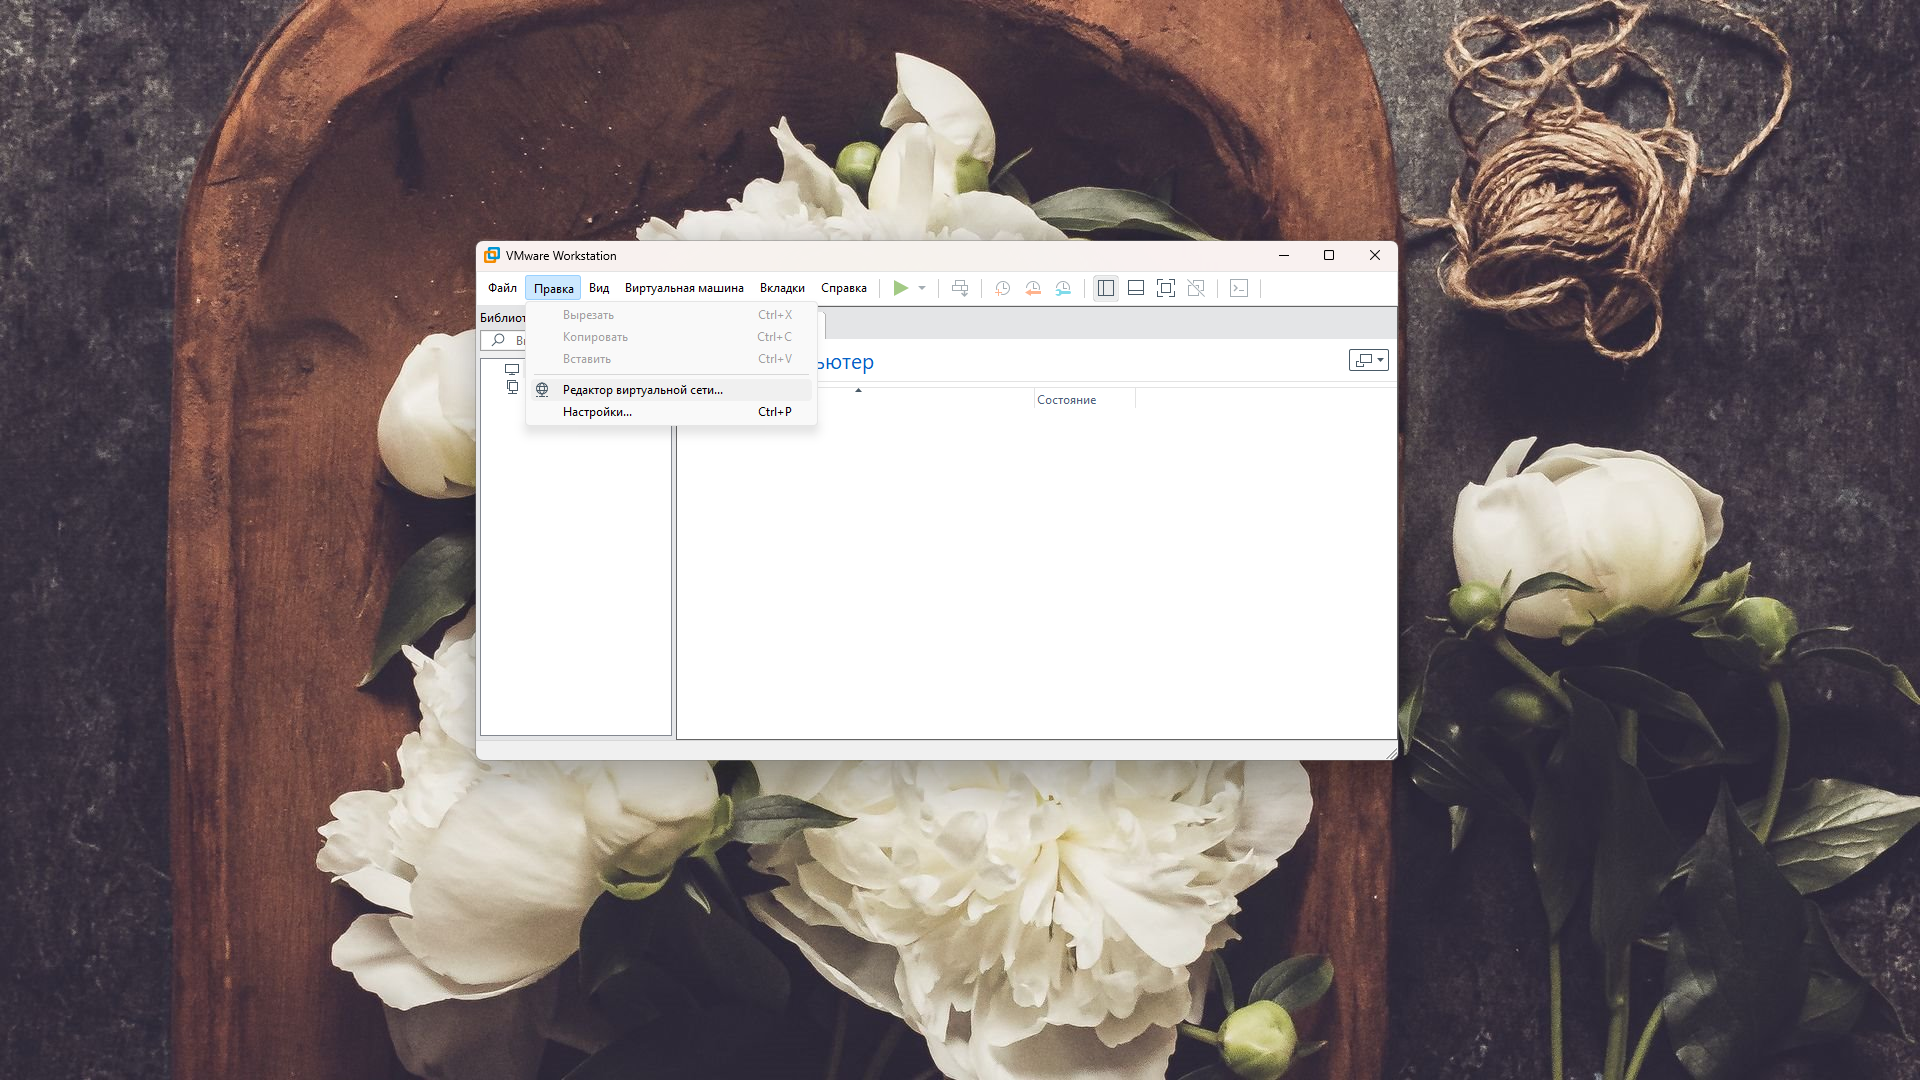
\includegraphics[width=0.85\textwidth]{03_00 (2)}
    \caption{Открываем редактор виртуальной сети}
    \label{img:2}
  \end{figure}

  \textit{VMware} редактирует системные сетевые интерфейсы, поэтому ему требуются
  дополнительные права - их можно выдать, нажав на кнопку "Изменить параметры":

  \begin{figure}[H]
    \centering
    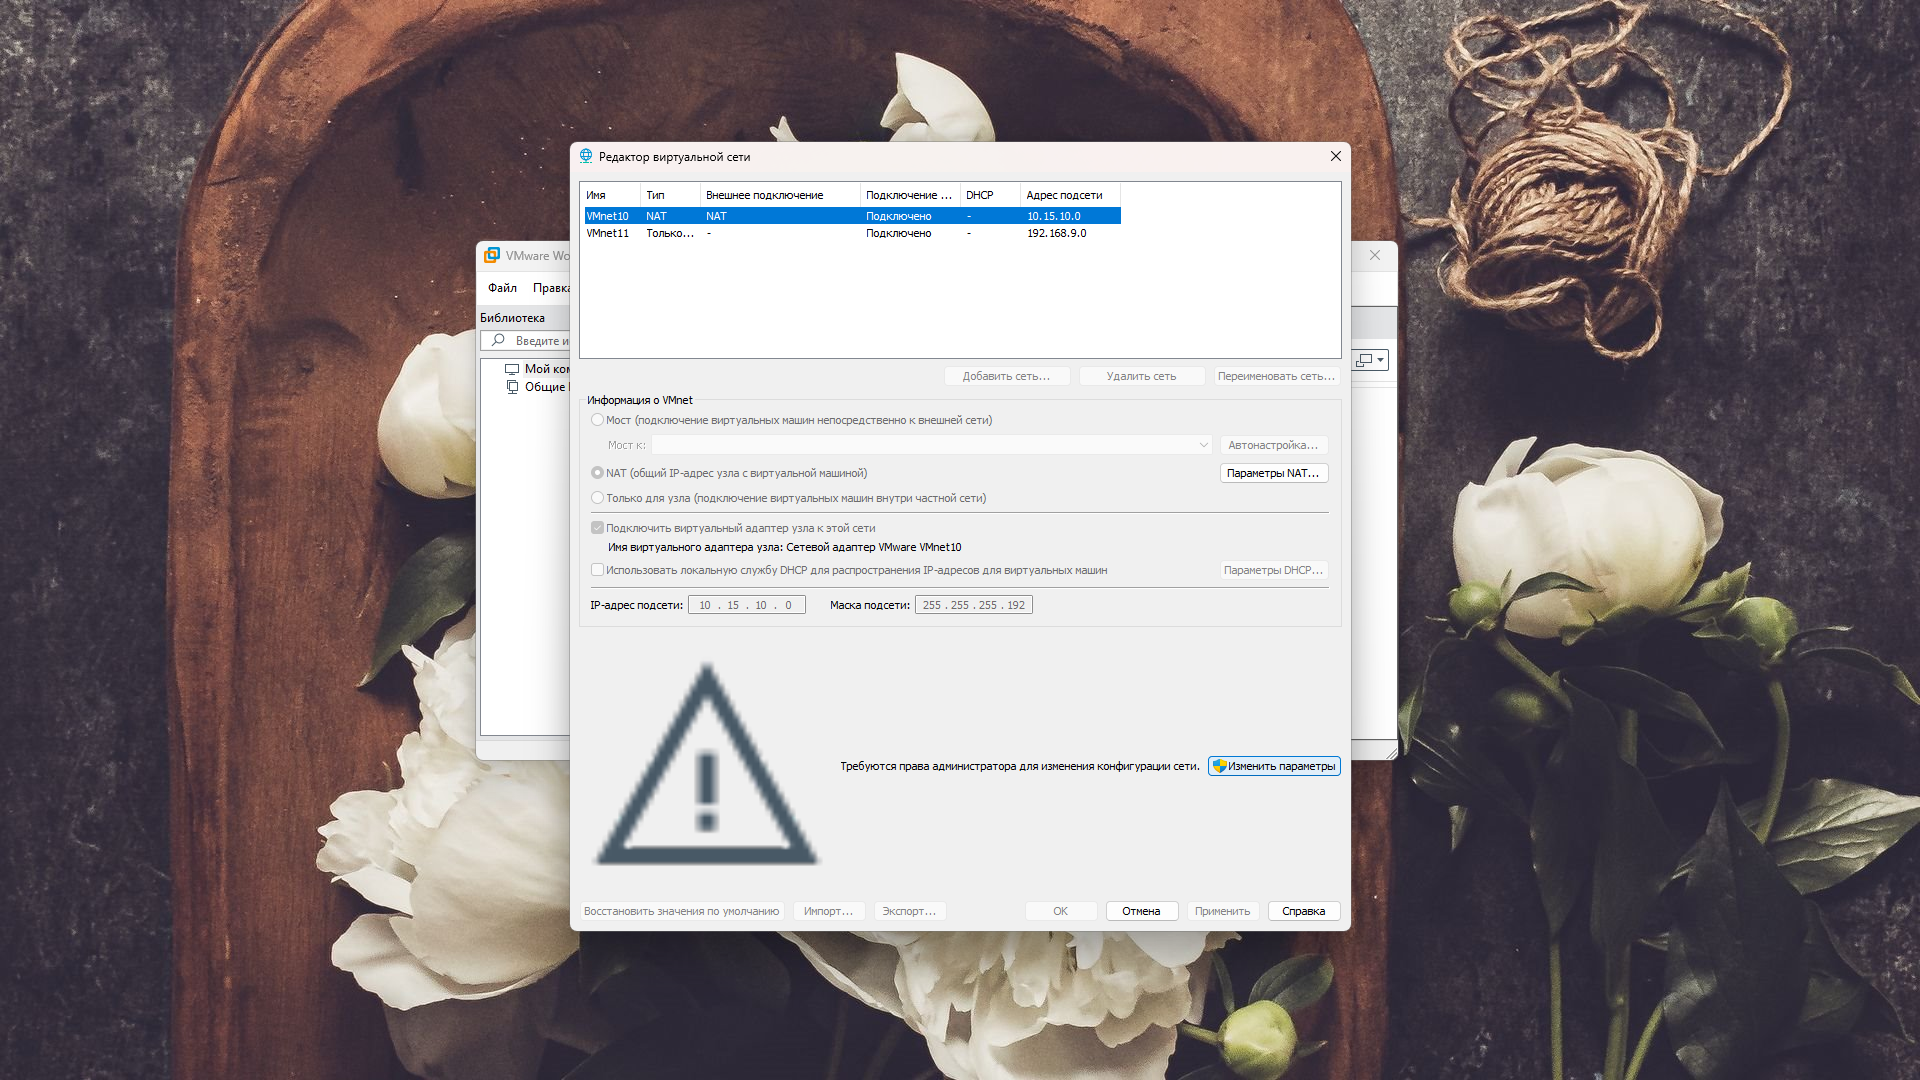
\includegraphics[width=0.85\textwidth]{03_00 (3)}
    \caption{Разрешим редактирование параметров}
    \label{img:3}
  \end{figure}

  Теперь нужно создать новую сеть, для этого воспользуемся кнопкой "Доавить сеть...":

  \begin{figure}[H]
    \centering
    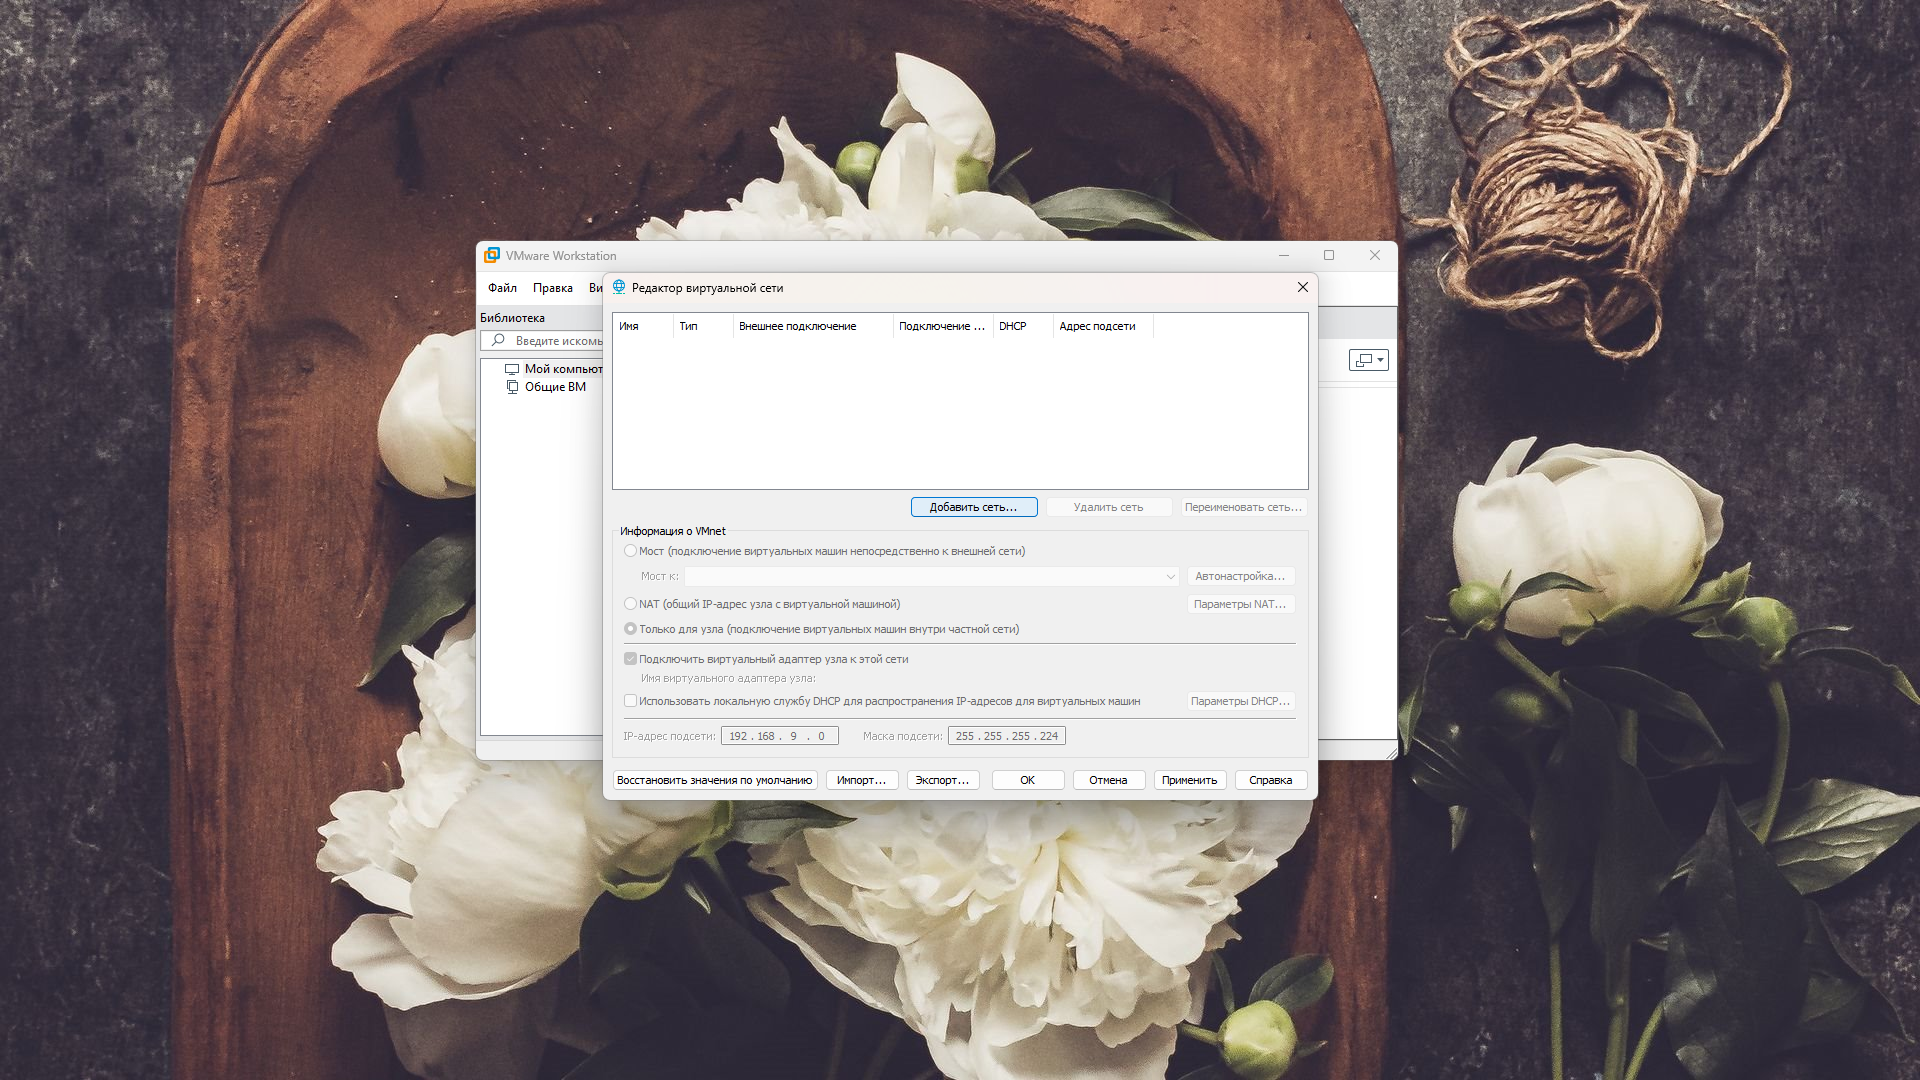
\includegraphics[width=0.85\textwidth]{03_00 (4)}
    \caption{Начинаем создание новой сети}
    \label{img:4}
  \end{figure}

  \begin{figure}[H]
    \centering
    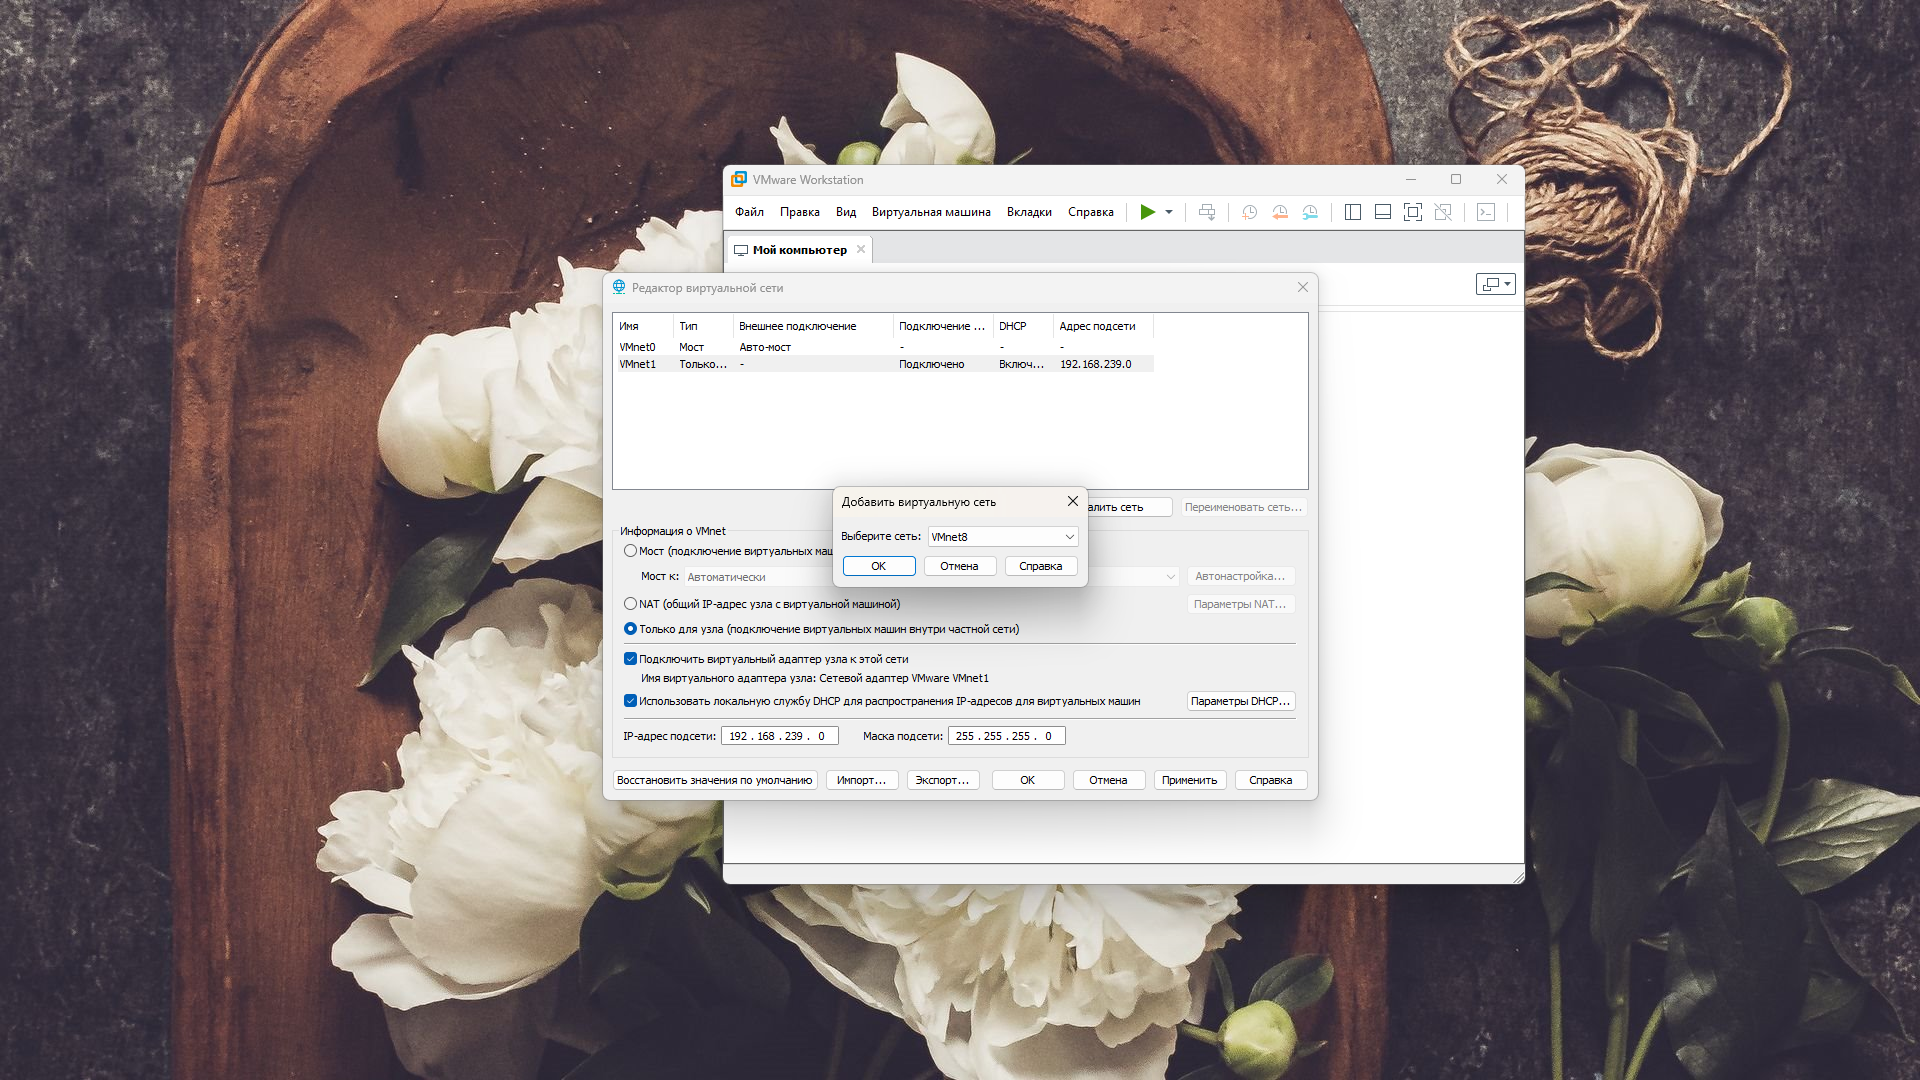
\includegraphics[width=0.85\textwidth]{03_01_00 (4)}
    \caption{Указываем имя новой сети}
    \label{img:5}
  \end{figure}

  Для новой сети было установлено имя \textit{VMnet8}, по нему дальше будет
  производиться подключение сетевых адаптеров.

  Теперь нужно сконфигурировать только что созданную сеть - установить для нее
  тип \textit{NAT}, а также включить встроенный \textit{DHCP} сервер, чтобы
  все машины автоматически получили уникальные в рамках данной сети адреса:

  \begin{figure}[H]
    \centering
    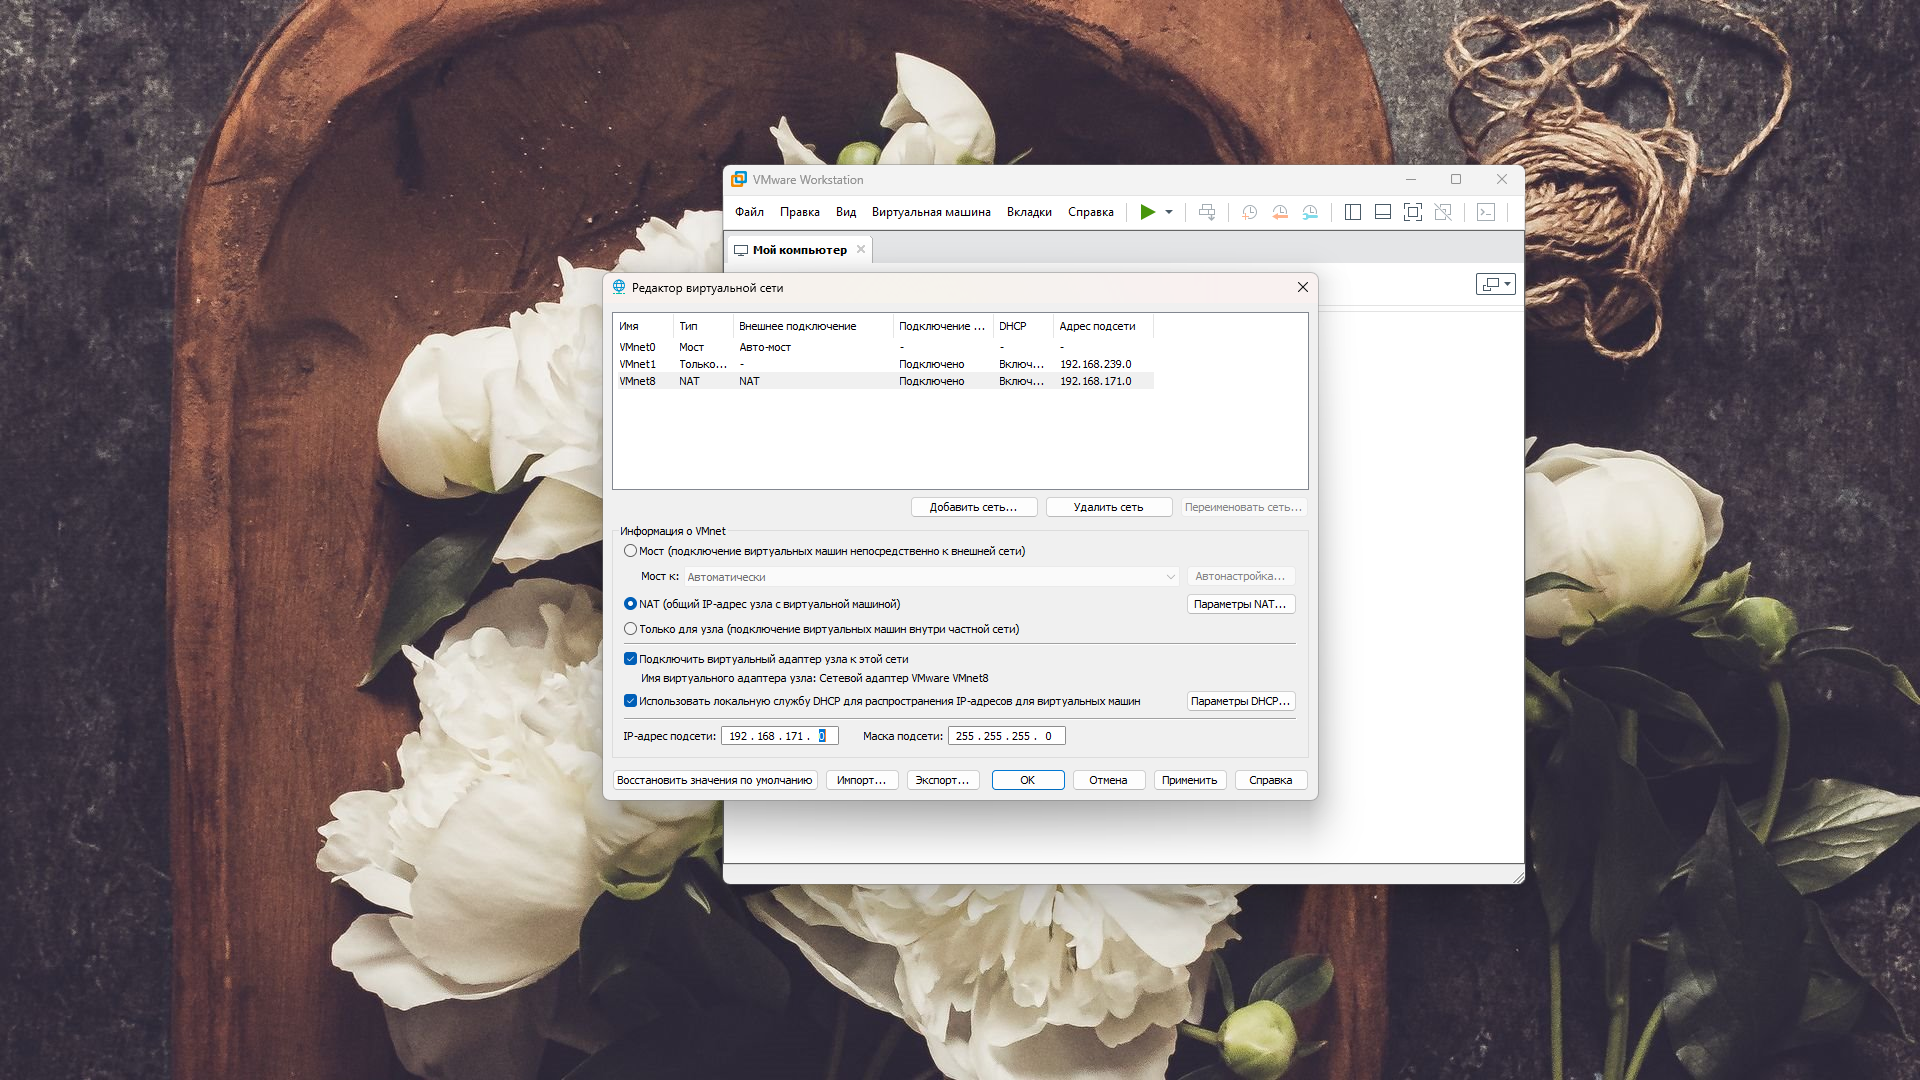
\includegraphics[width=0.85\textwidth]{03_01_00 (3)}
    \caption{Конфигурация новой \textit{NAT} сети}
    \label{img:6}
  \end{figure}

  Возможно пригодиться узнать адрес шлюза по умолчанию (он же в данном случае
  адрес базового \textit{DNS} сервера) - это можно сделать провалившись
  в меню "Параметры NAT":

  \begin{figure}[H]
    \centering
    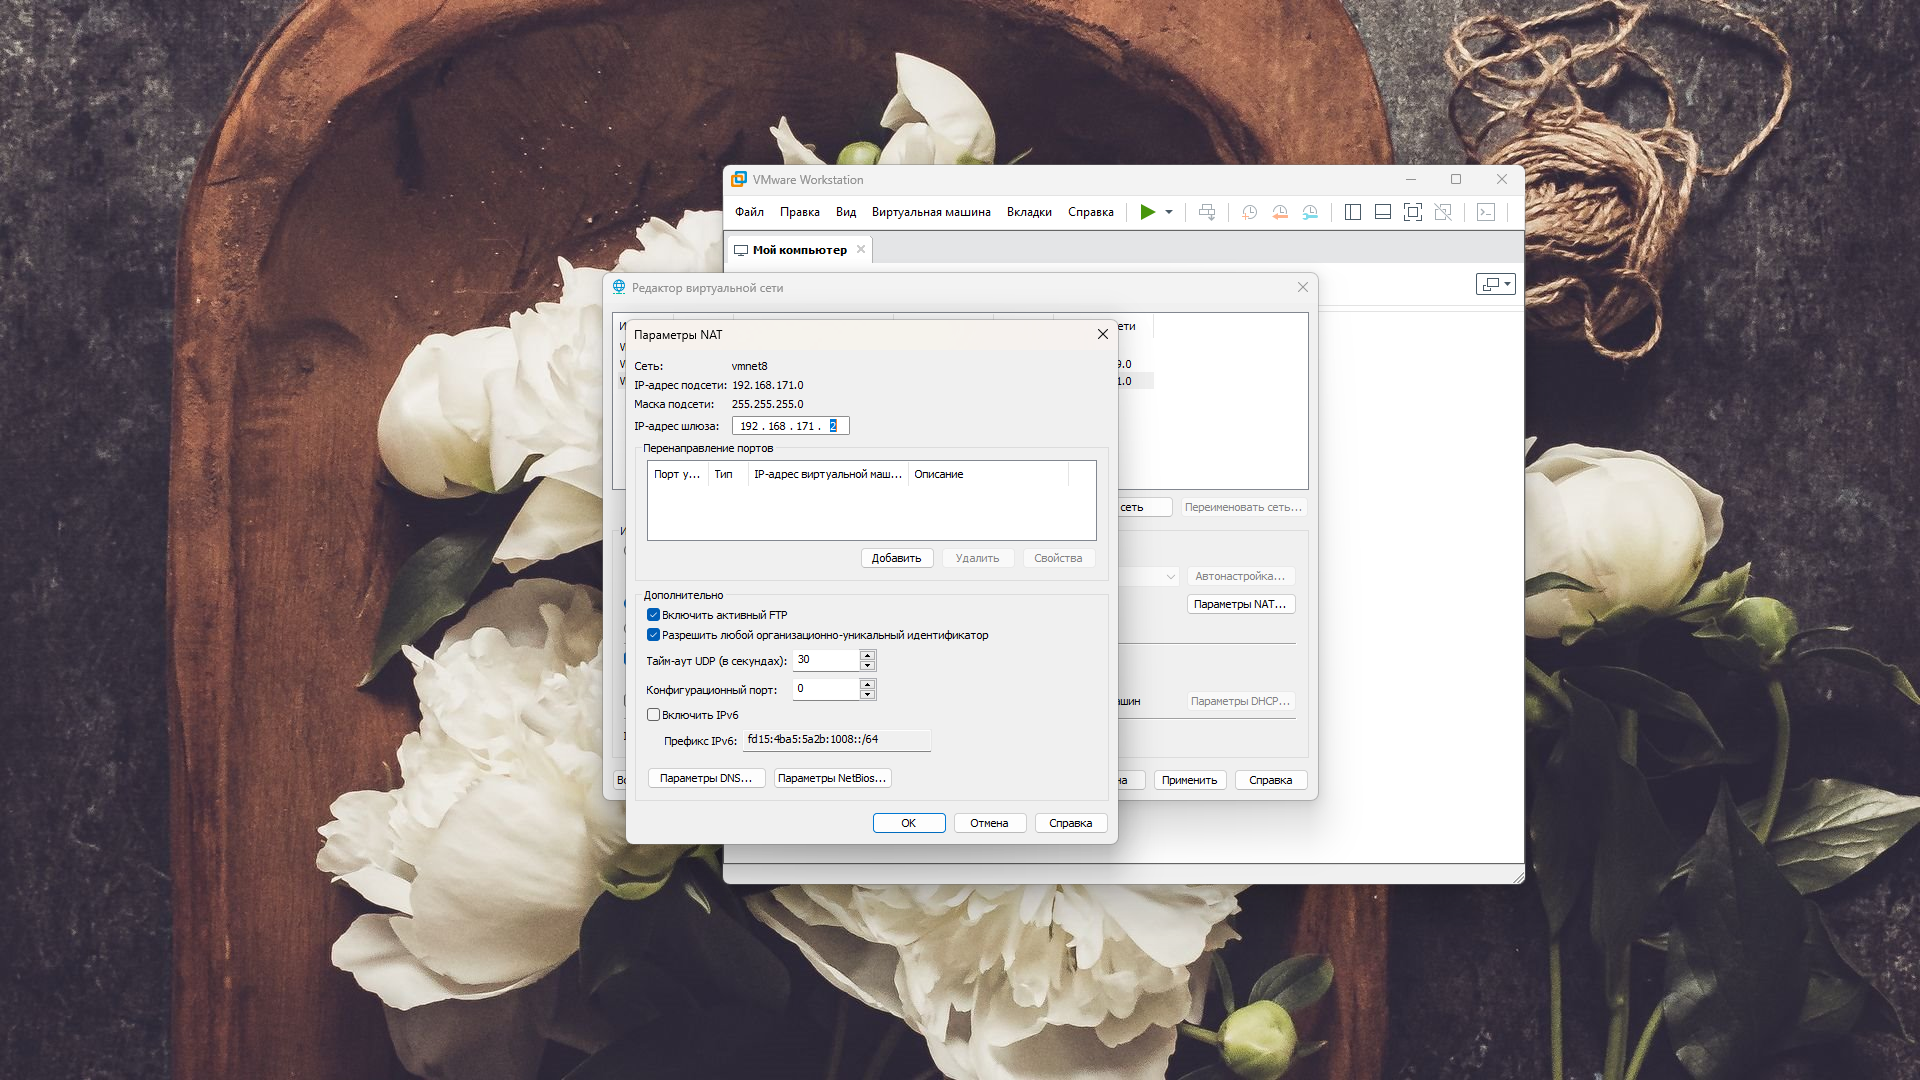
\includegraphics[width=0.85\textwidth]{03_01_00 (2)}
    \caption{Параметры сети}
    \label{img:7}
  \end{figure}

  Видно, что адрес шлюза по умолчанию 192.168.171.2.

  \subsubsection{Создание виртуальных машин}

  Для выполнения работы необходима атакующая и атакуемая машины, начнем их
  создание. За основу первой машины будет использован уже готовый слепок системы,
  необходимо только открыть его:
  
  \begin{figure}[H]
    \centering
    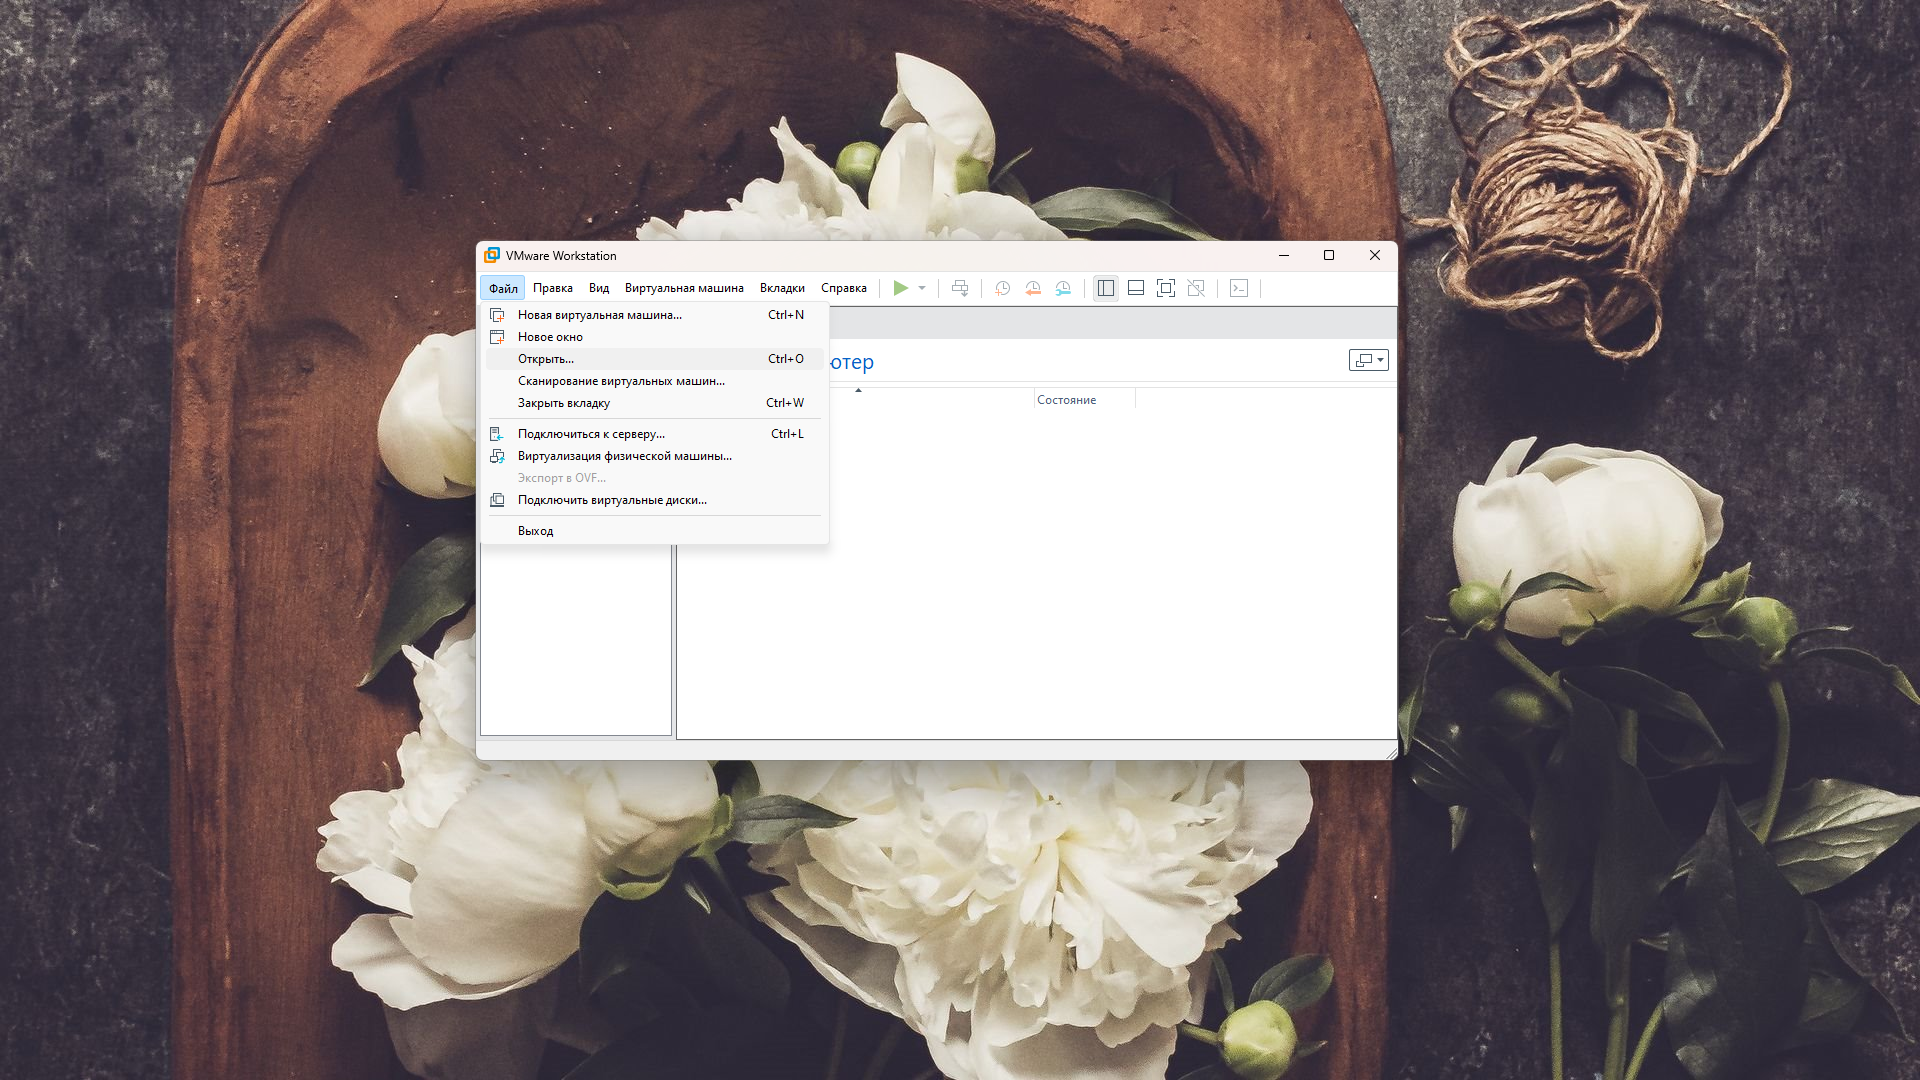
\includegraphics[width=0.85\textwidth]{03_00 (7)}
    \caption{Выбираем пункт "Открыть"}
    \label{img:7_5}
  \end{figure}

  \begin{figure}[H]
    \centering
    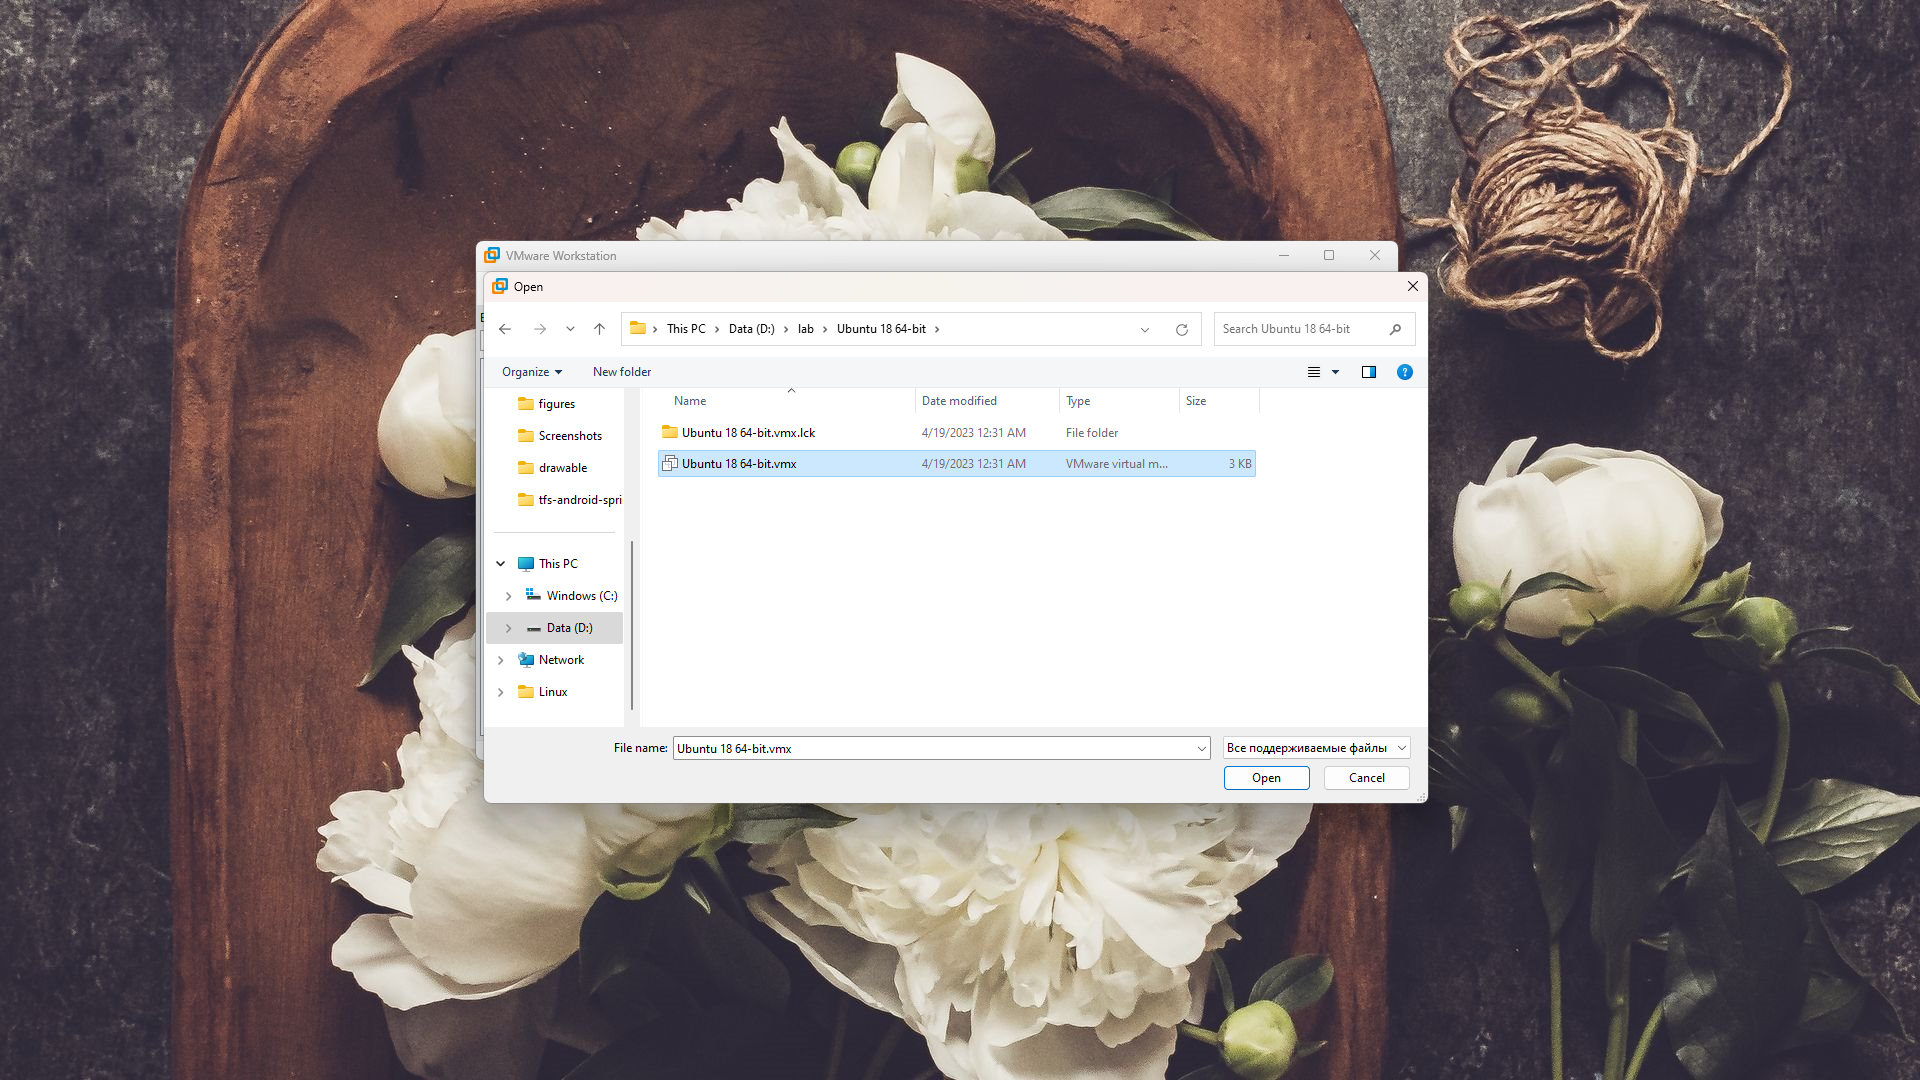
\includegraphics[width=0.85\textwidth]{03_00 (8)}
    \caption{Указываем образ нужной нам системы}
    \label{img:8}
  \end{figure}

  После окончания открытия образа необходимо подключить машину к необходимой сети,
  для этого заходим в пункт "Изменить параметры":

  \begin{figure}[H]
    \centering
    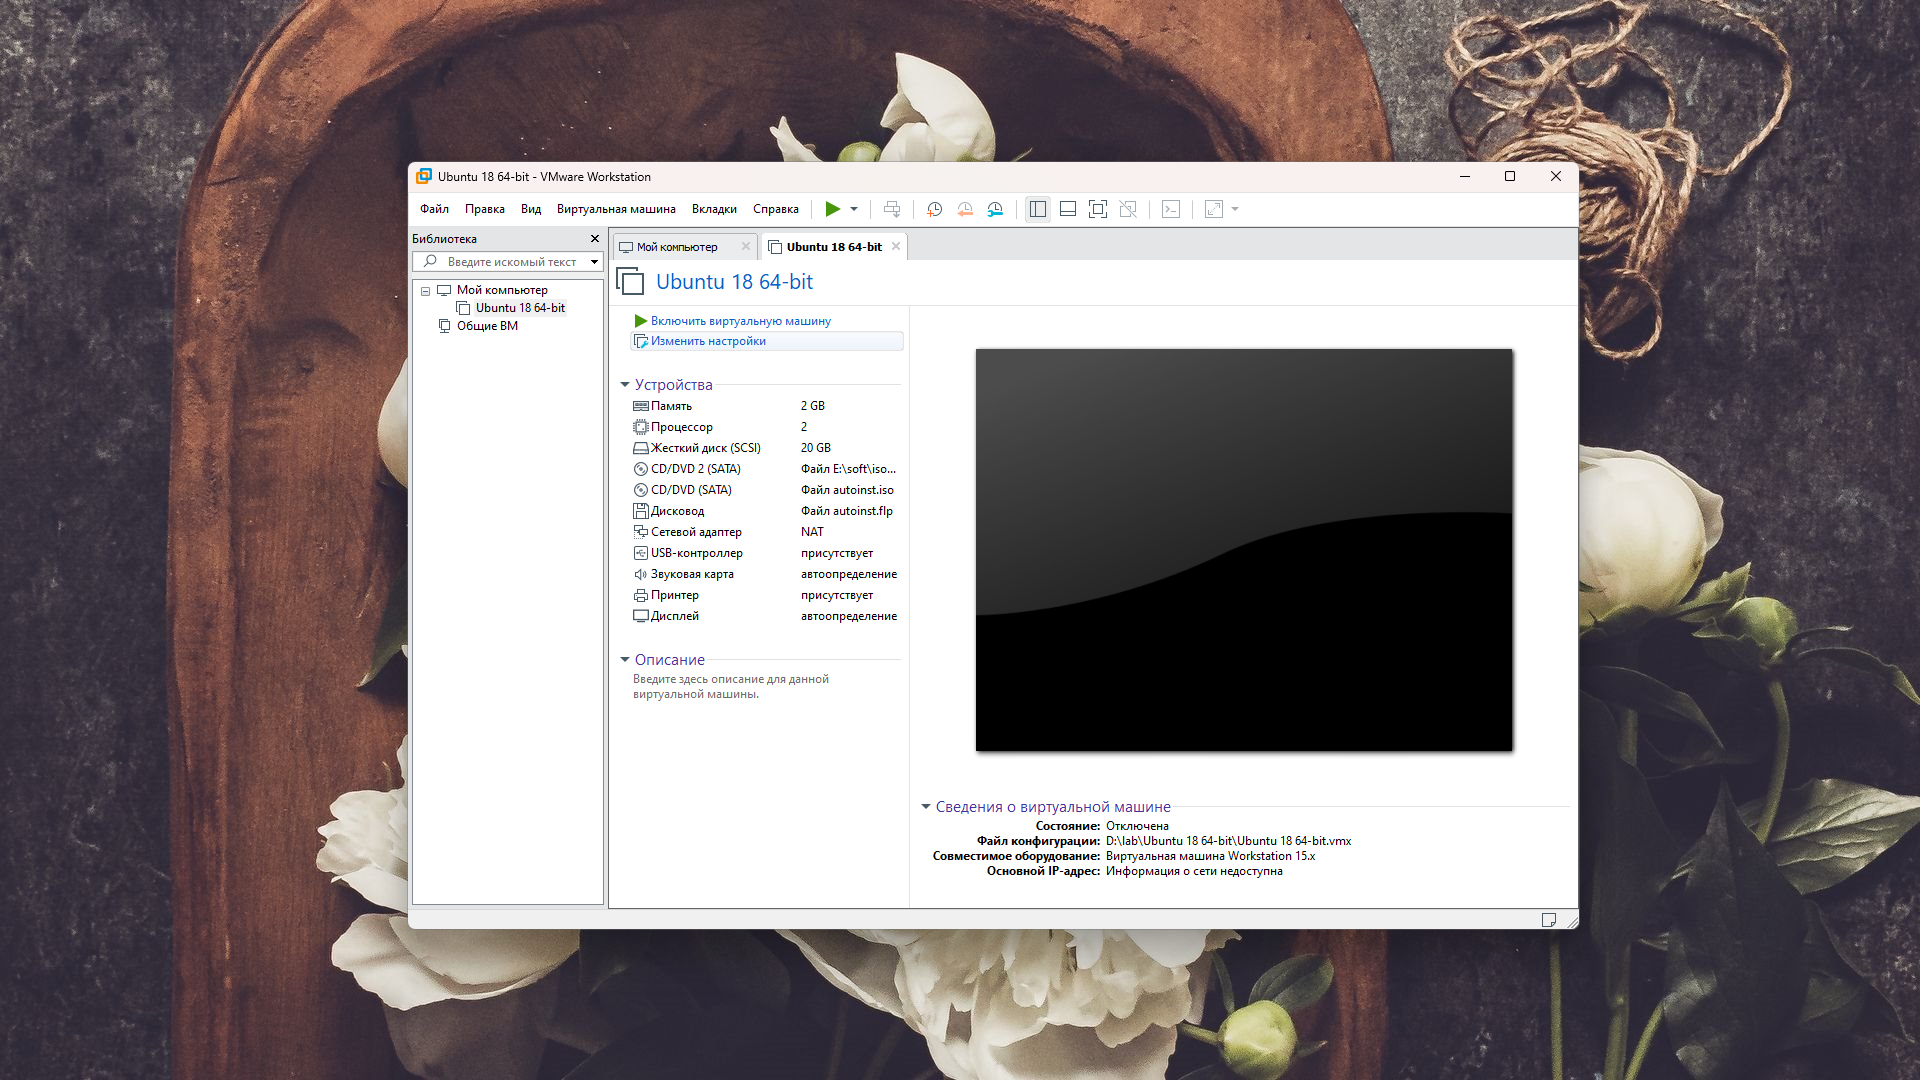
\includegraphics[width=0.85\textwidth]{03_00 (9)}
    \caption{Конфигурирование ВМ}
    \label{img:9}
  \end{figure}

  Чтобы произвести подключение к сети, необходим сетевой адаптер - создадим его:

  \begin{figure}[H]
    \centering
    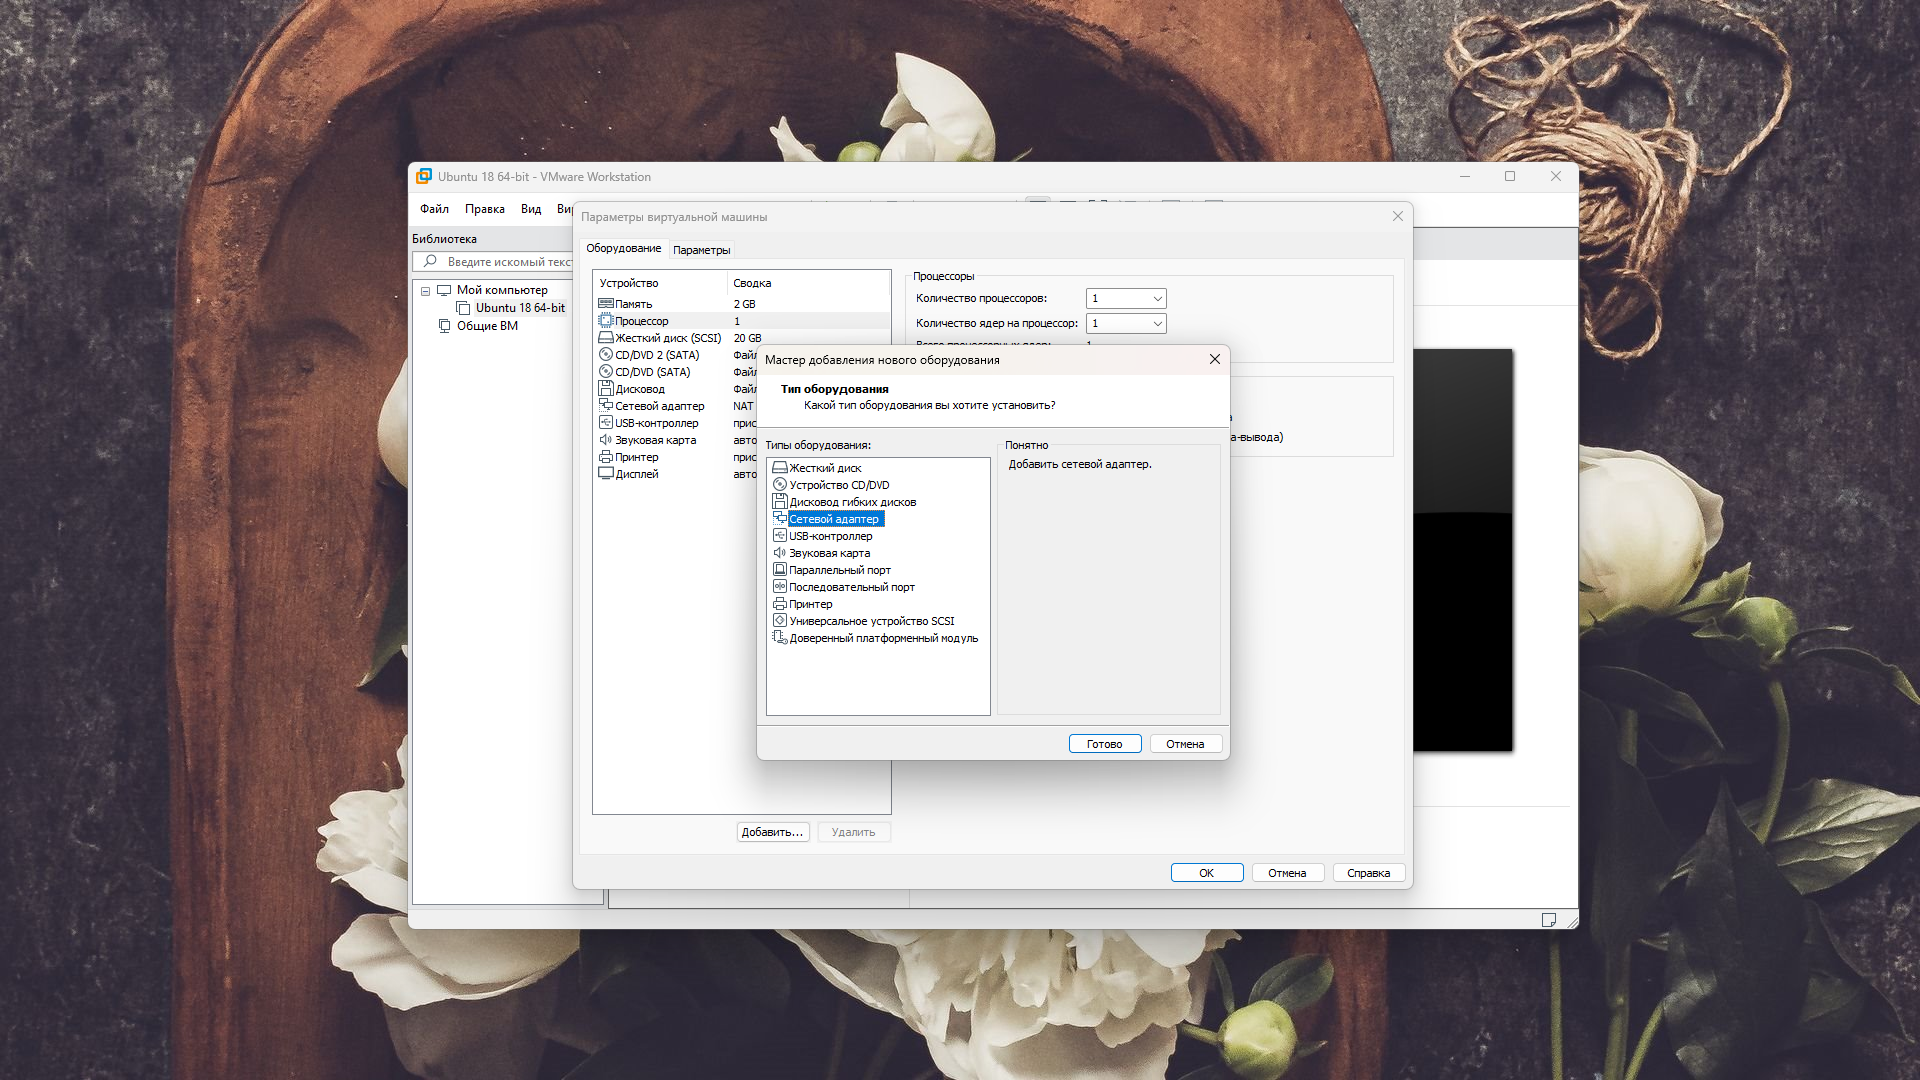
\includegraphics[width=0.85\textwidth]{03_00 (10)}
    \caption{Создание сетевого адаптера}
    \label{img:10}
  \end{figure}

  Далее этот адаптер необходимо привязать к нужной сети - выбираем ее из списка:

  \begin{figure}[H]
    \centering
    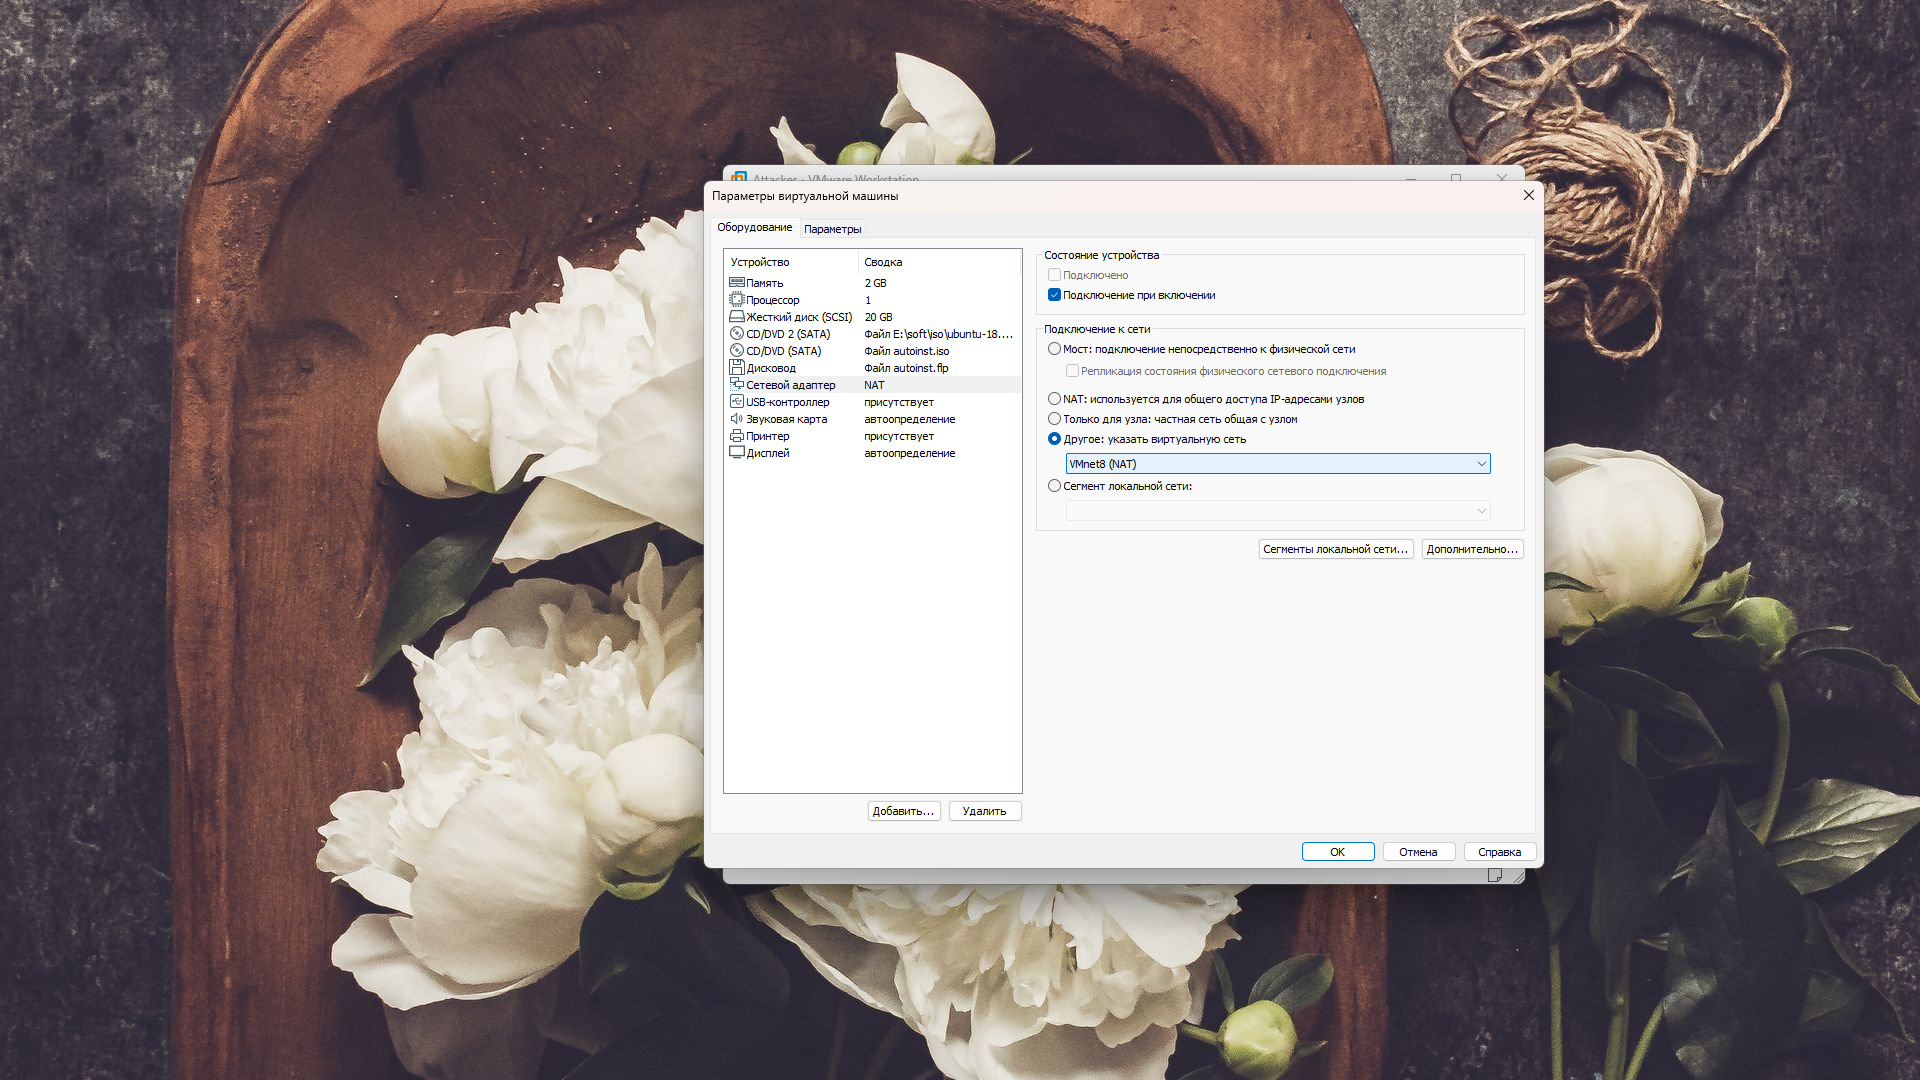
\includegraphics[width=0.85\textwidth]{03_00 (11)}
    \caption{Выбираем нужную сеть (VMNet8)}
    \label{img:11}
  \end{figure}

  В итоге имеем одну виртуальную машину, подключенную к сети \textit{NAT}.
  Чтобы не путаться, изменим ее имя на \textit{Attacker} и в дальнейшем будем
  использовать как атакующую:

  \begin{figure}[H]
    \centering
    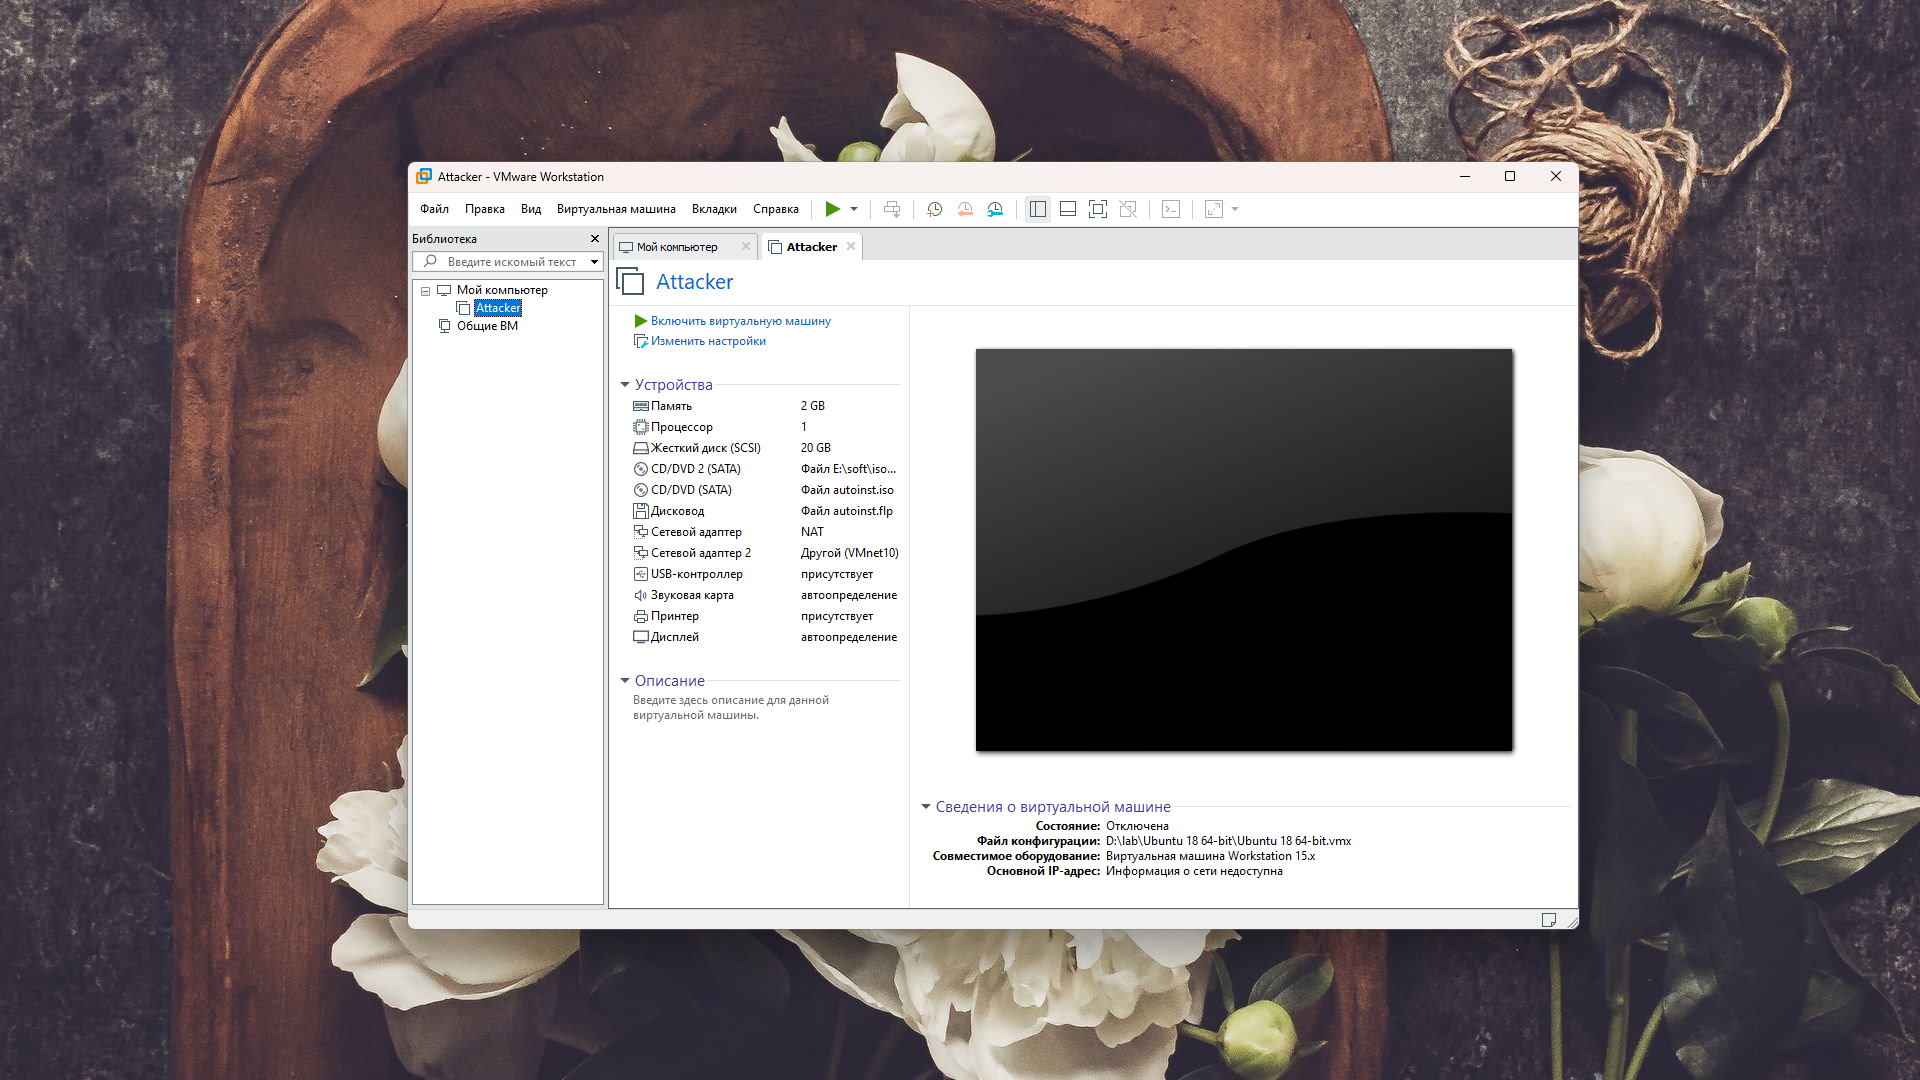
\includegraphics[width=0.85\textwidth]{03_00 (12)}
    \caption{Итоговая атакующая ВМ}
    \label{img:12}
  \end{figure}

  Также необходима и атакуемая машина - создадим ее клонированием атакующей:

  \begin{figure}[H]
    \centering
    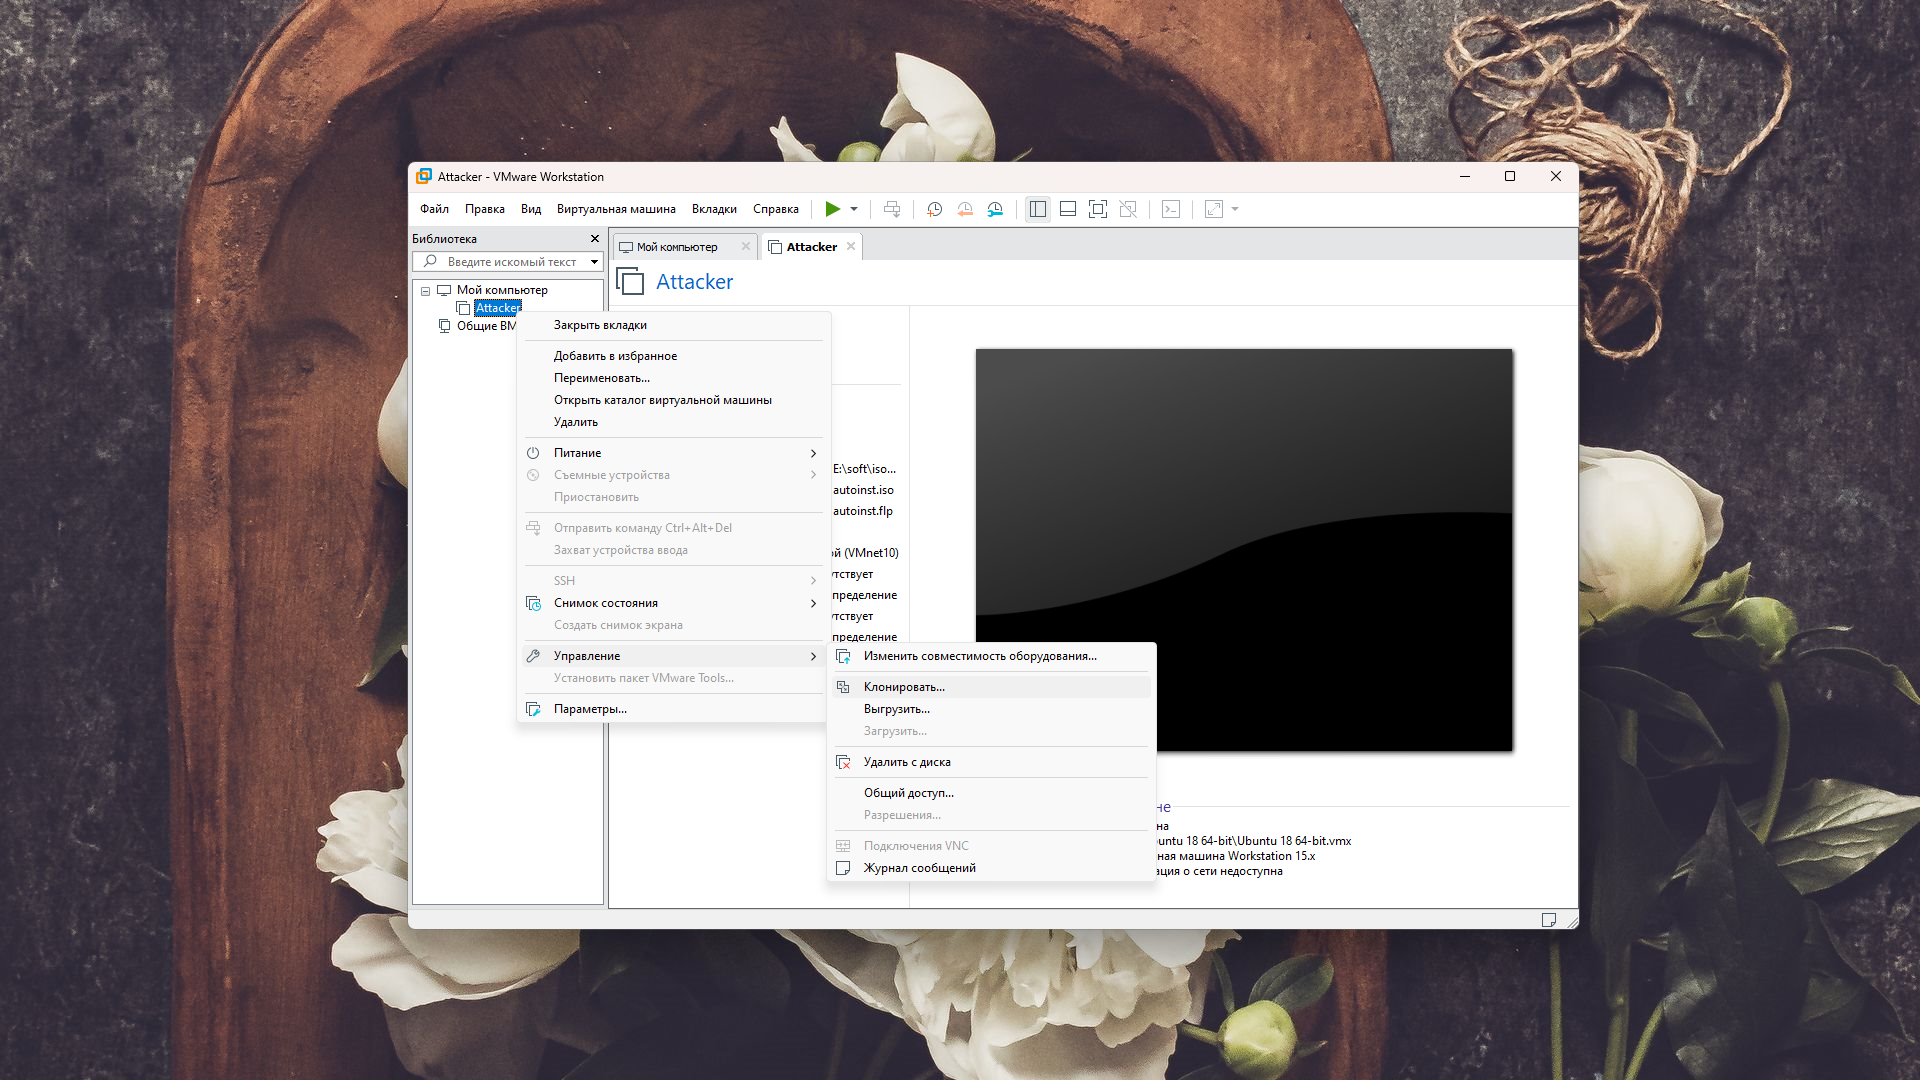
\includegraphics[width=0.85\textwidth]{03_00 (13)}
    \caption{Начинаем клонирование}
    \label{img:13}
  \end{figure}

  \begin{figure}[H]
    \centering
    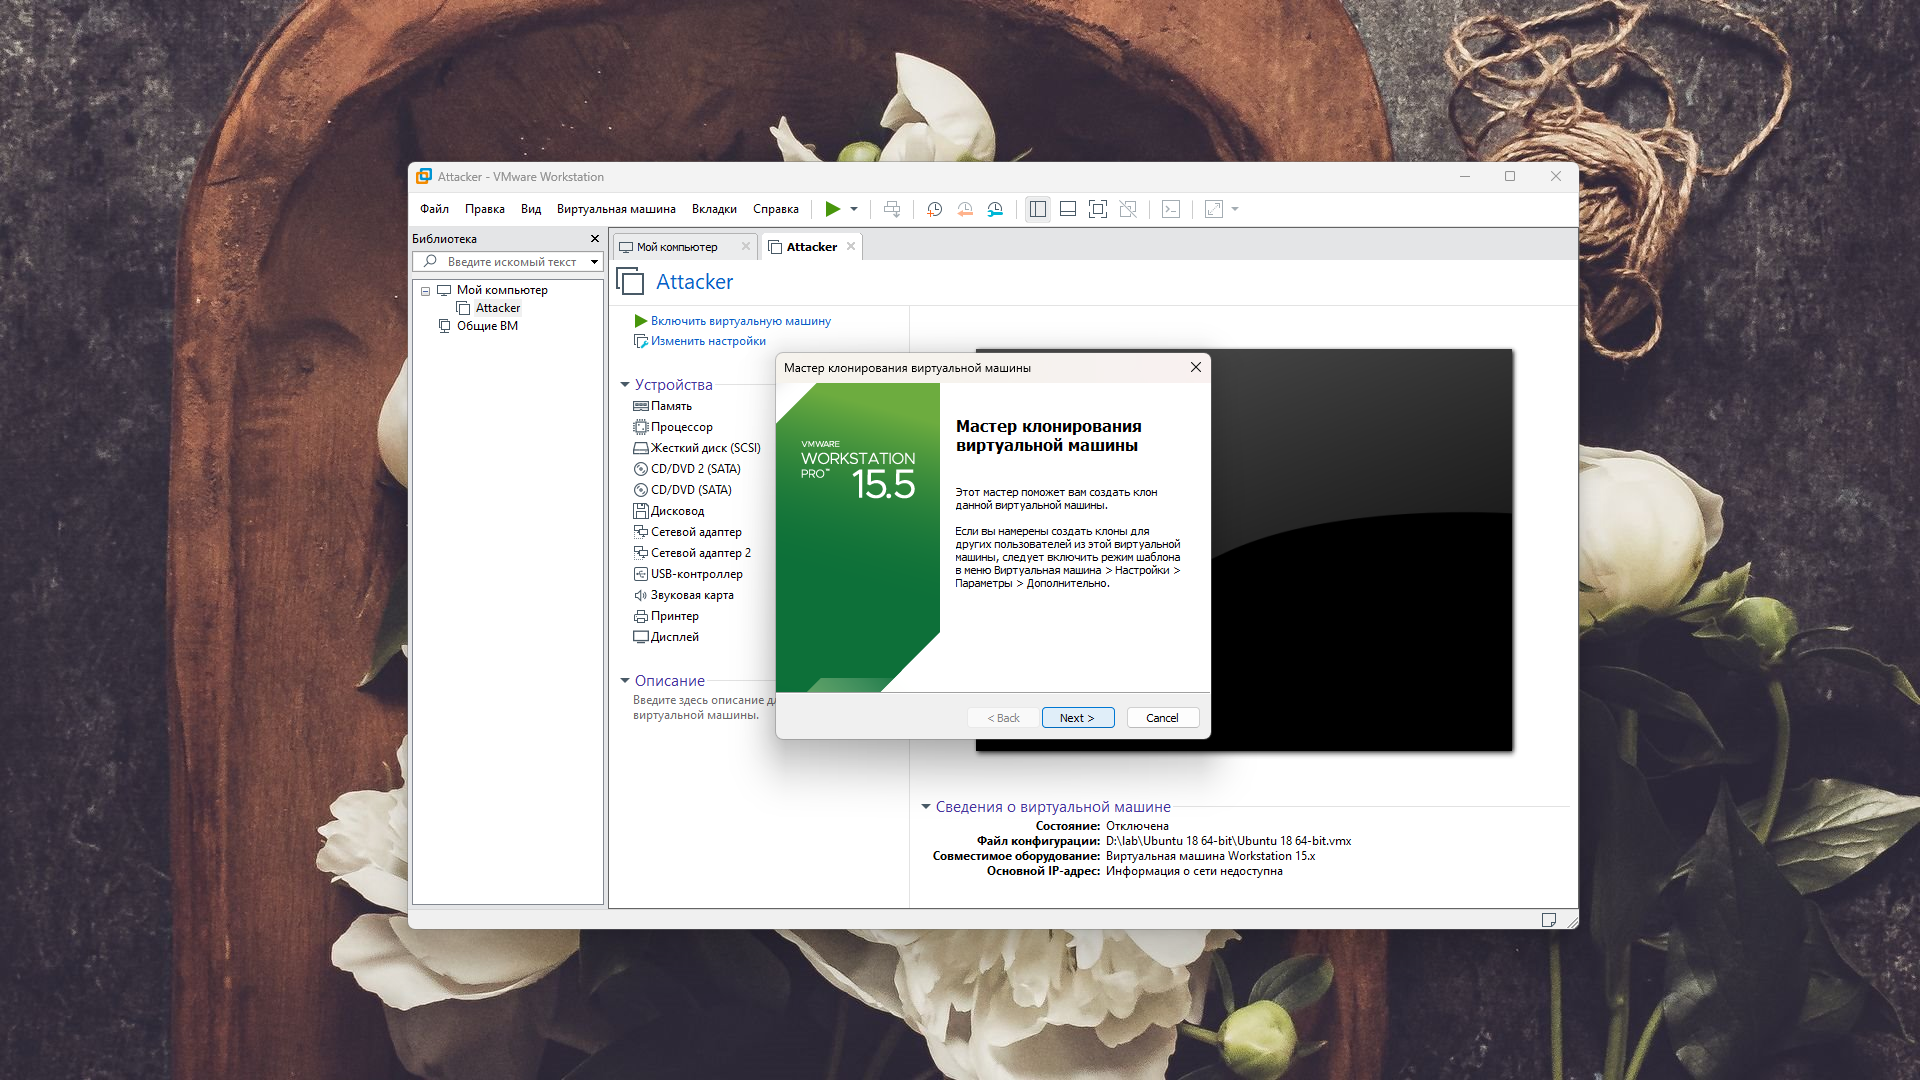
\includegraphics[width=0.85\textwidth]{03_00 (14)}
    \caption{Нажимем "Next >"}
    \label{img:14}
  \end{figure}

  \begin{figure}[H]
    \centering
    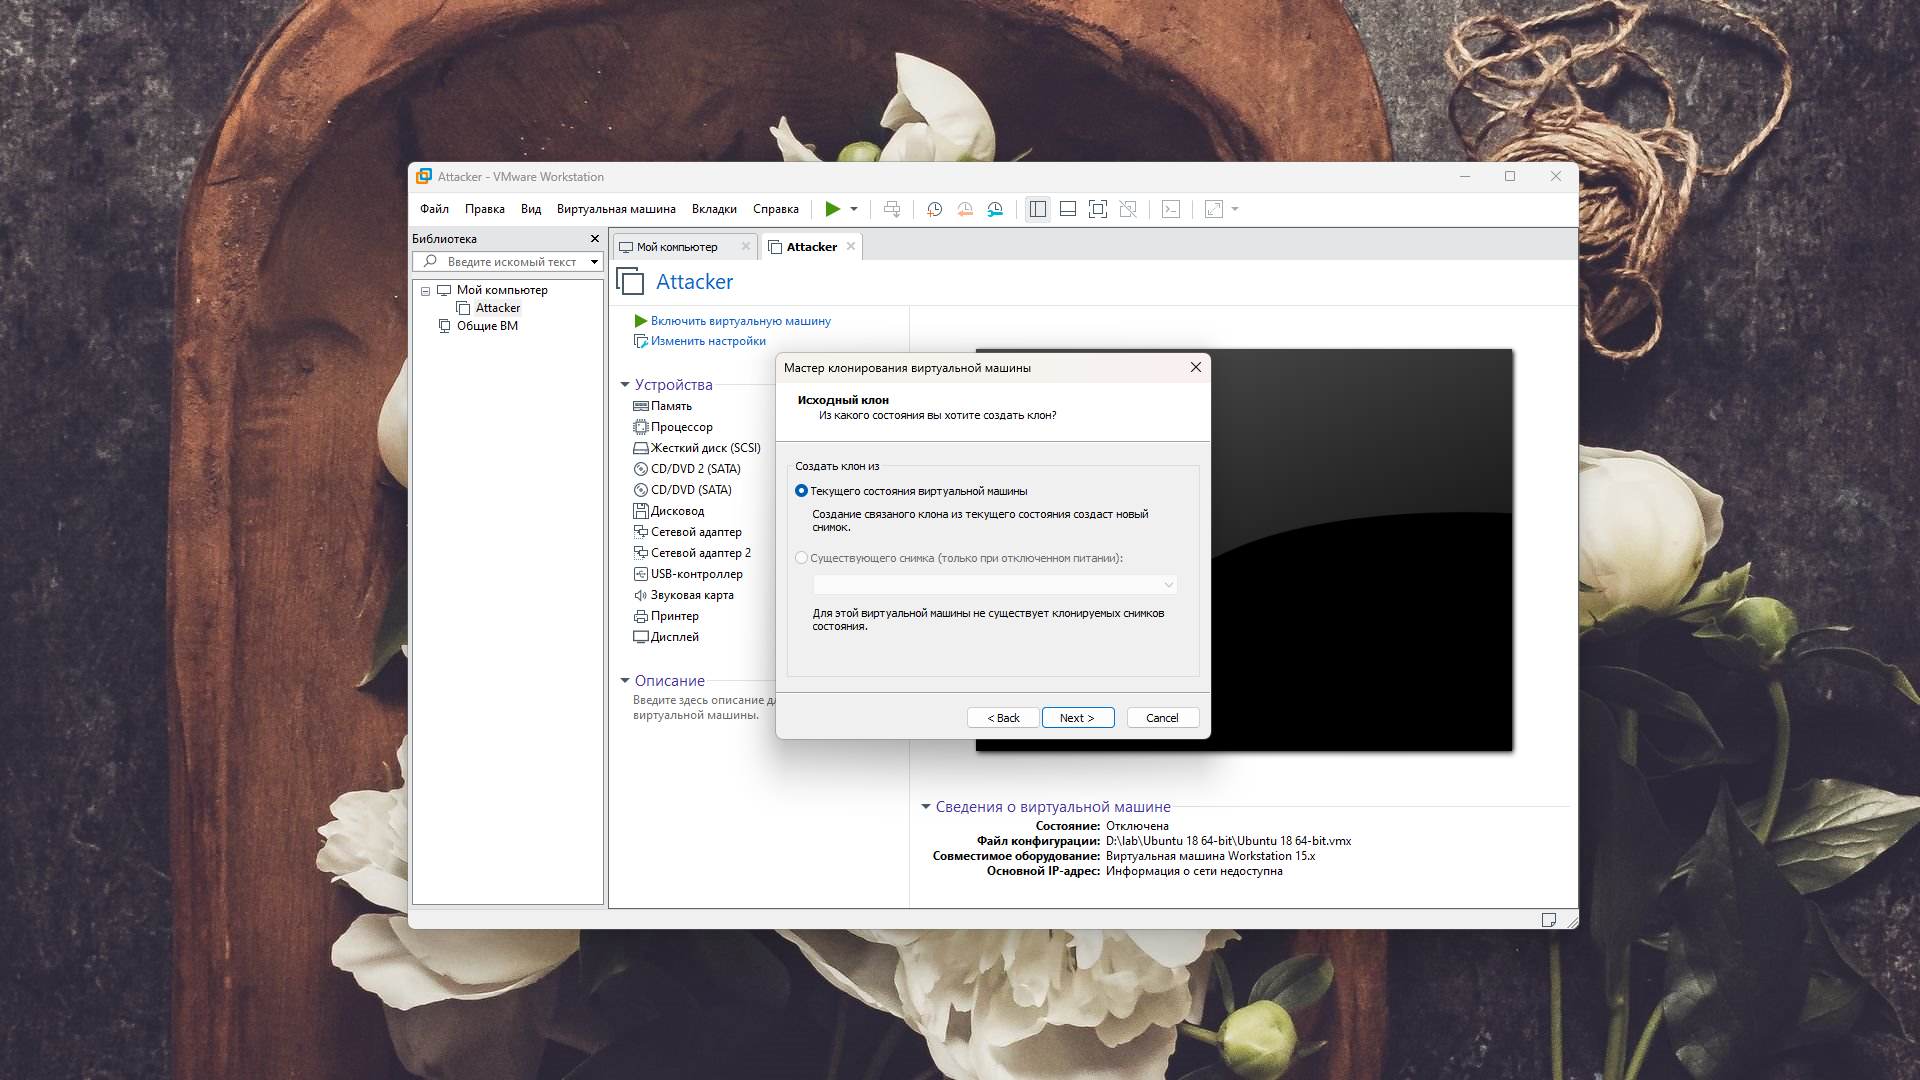
\includegraphics[width=0.85\textwidth]{03_00 (15)}
    \caption{Оставляем поля без изменений}
    \label{img:15}
  \end{figure}

  Чтобы уменьшить связанность атакуемой и атакующей машин между собой,
  создадим полные клон:

  \begin{figure}[H]
    \centering
    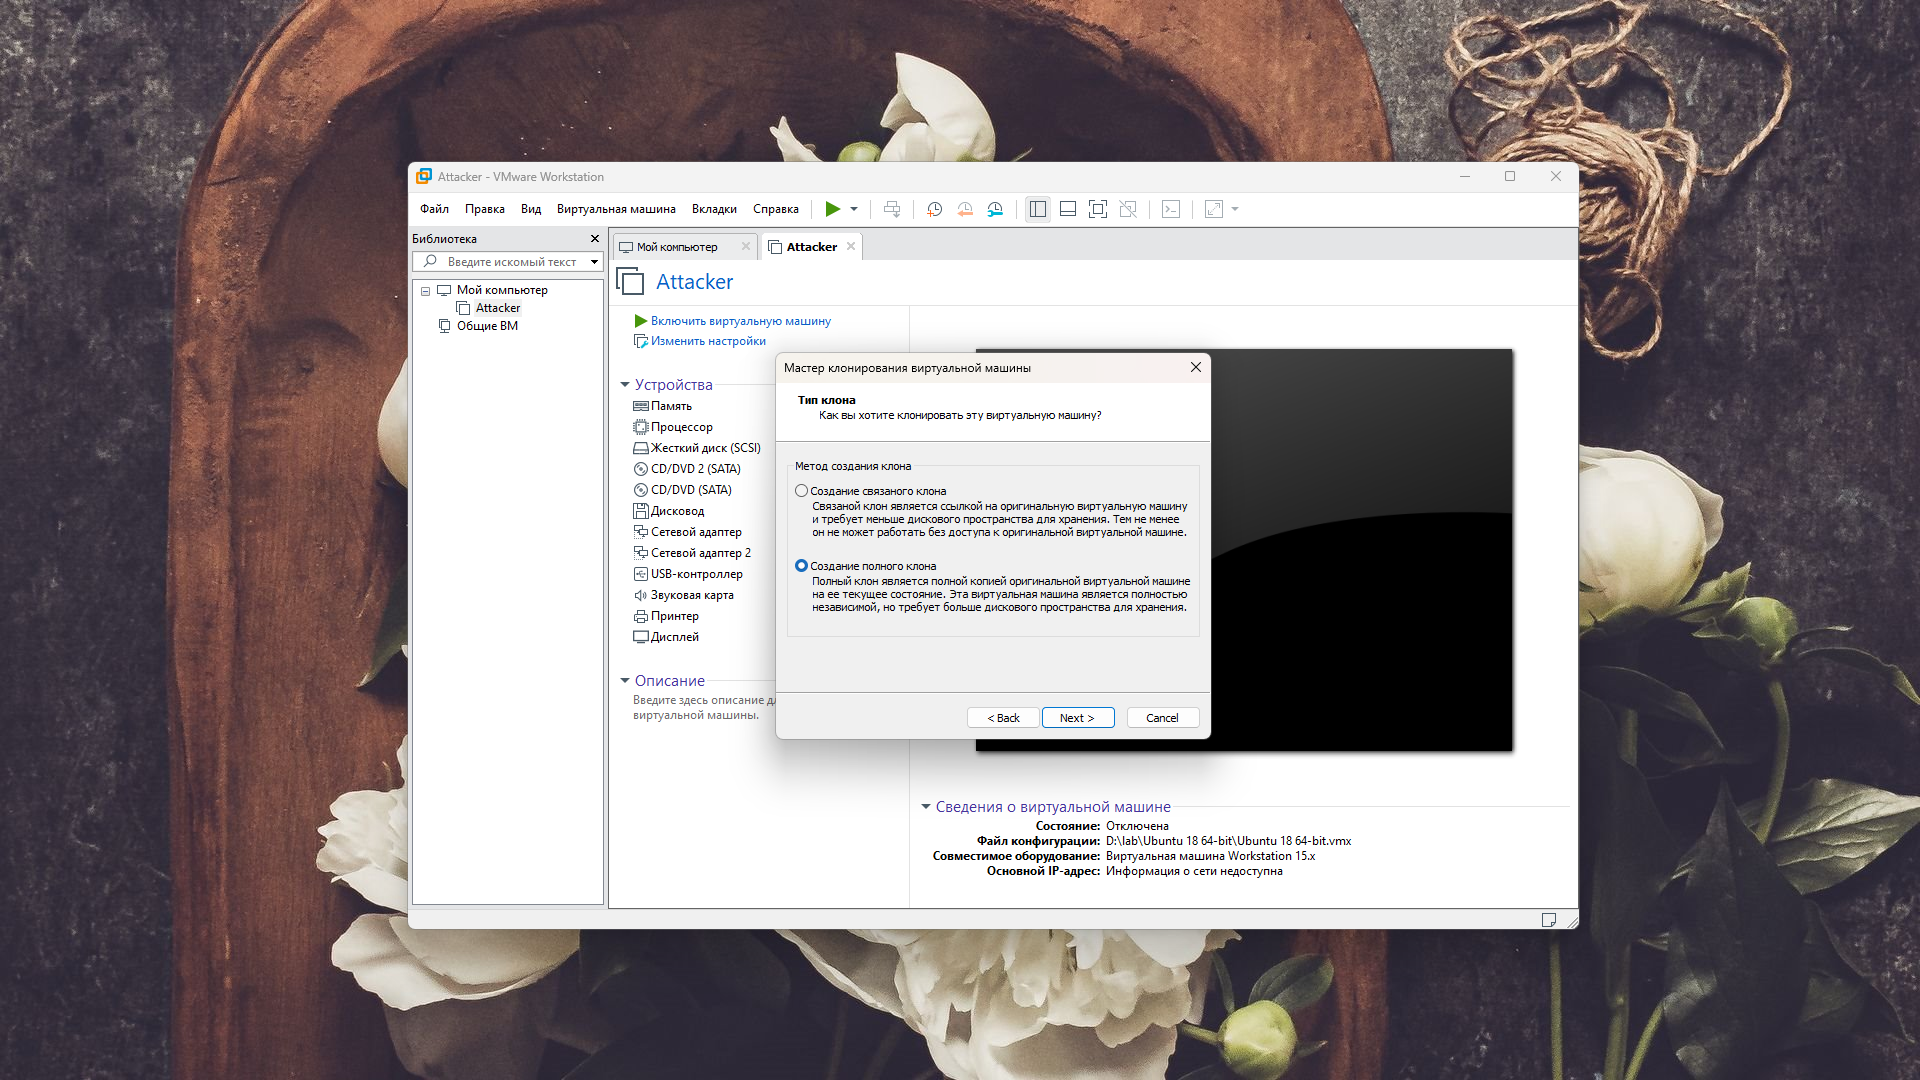
\includegraphics[width=0.85\textwidth]{03_00 (16)}
    \caption{Выбираем "Создание полного клона"}
    \label{img:16}
  \end{figure}

  Сразу же укажем правильное имя для новой машины - \textit{Defender}:

  \begin{figure}[H]
    \centering
    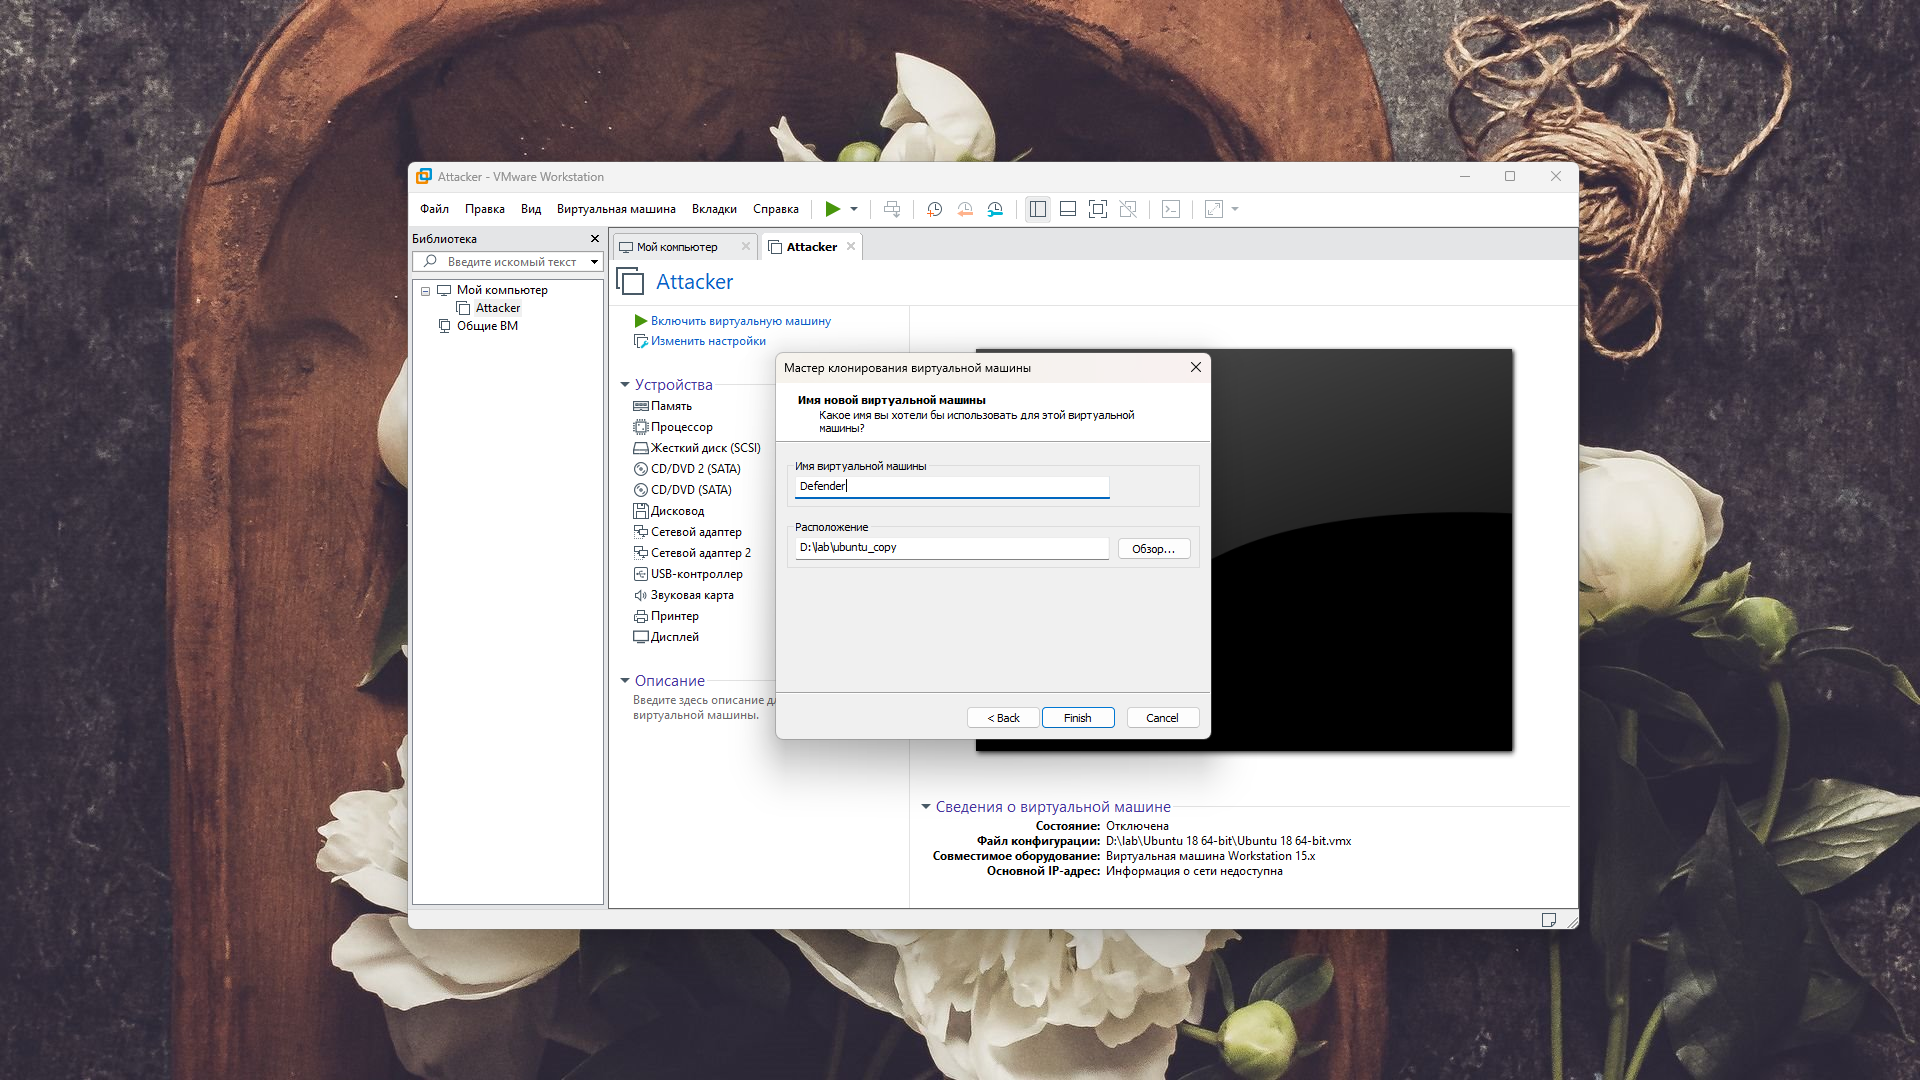
\includegraphics[width=0.85\textwidth]{03_00 (18)}
    \caption{Атакуемая машины}
    \label{img:18}
  \end{figure}

  \begin{figure}[H]
    \centering
    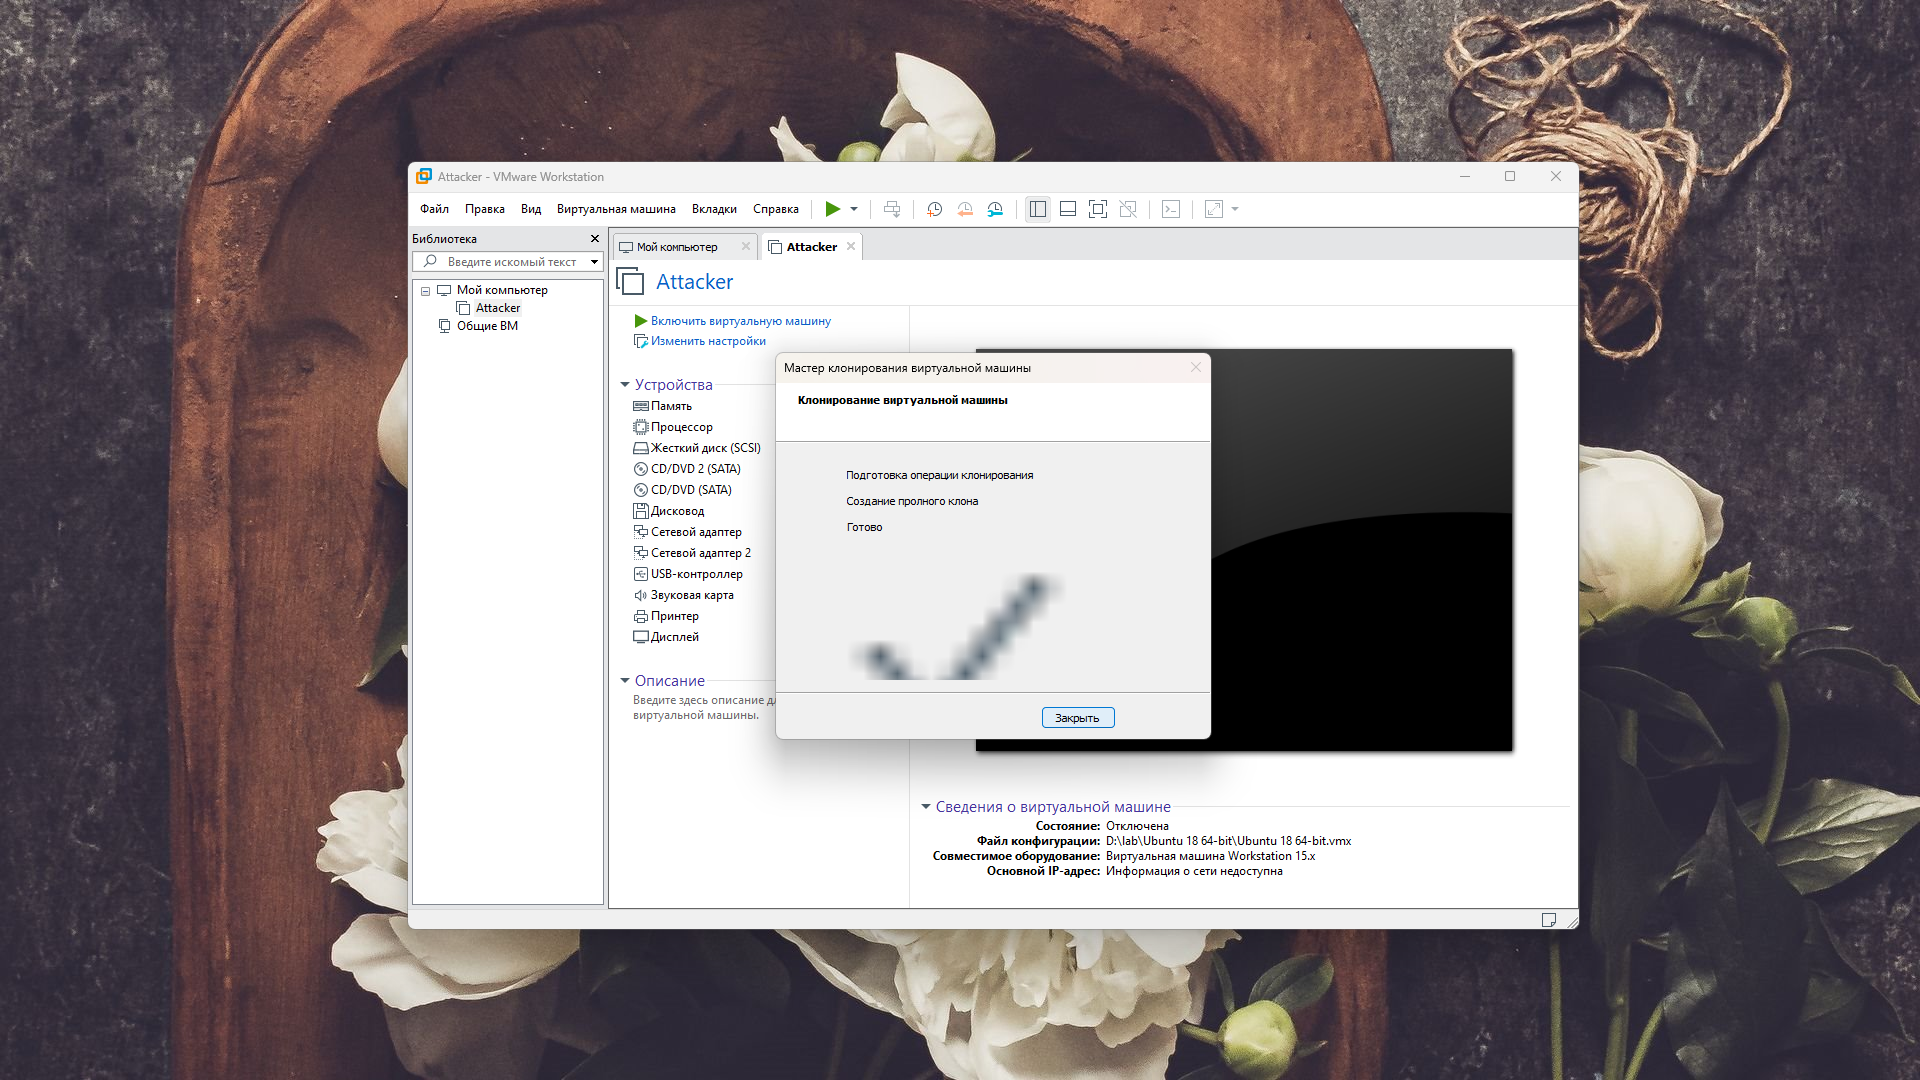
\includegraphics[width=0.85\textwidth]{03_00 (19)}
    \caption{Клонирование завершено}
    \label{img:19}
  \end{figure}

  Клонированная машина уже подключена к \textit{NAT} сети, поэтому дополнительная
  настройка сетевых адаптеров не требуется.

  \begin{figure}[H]
    \centering
    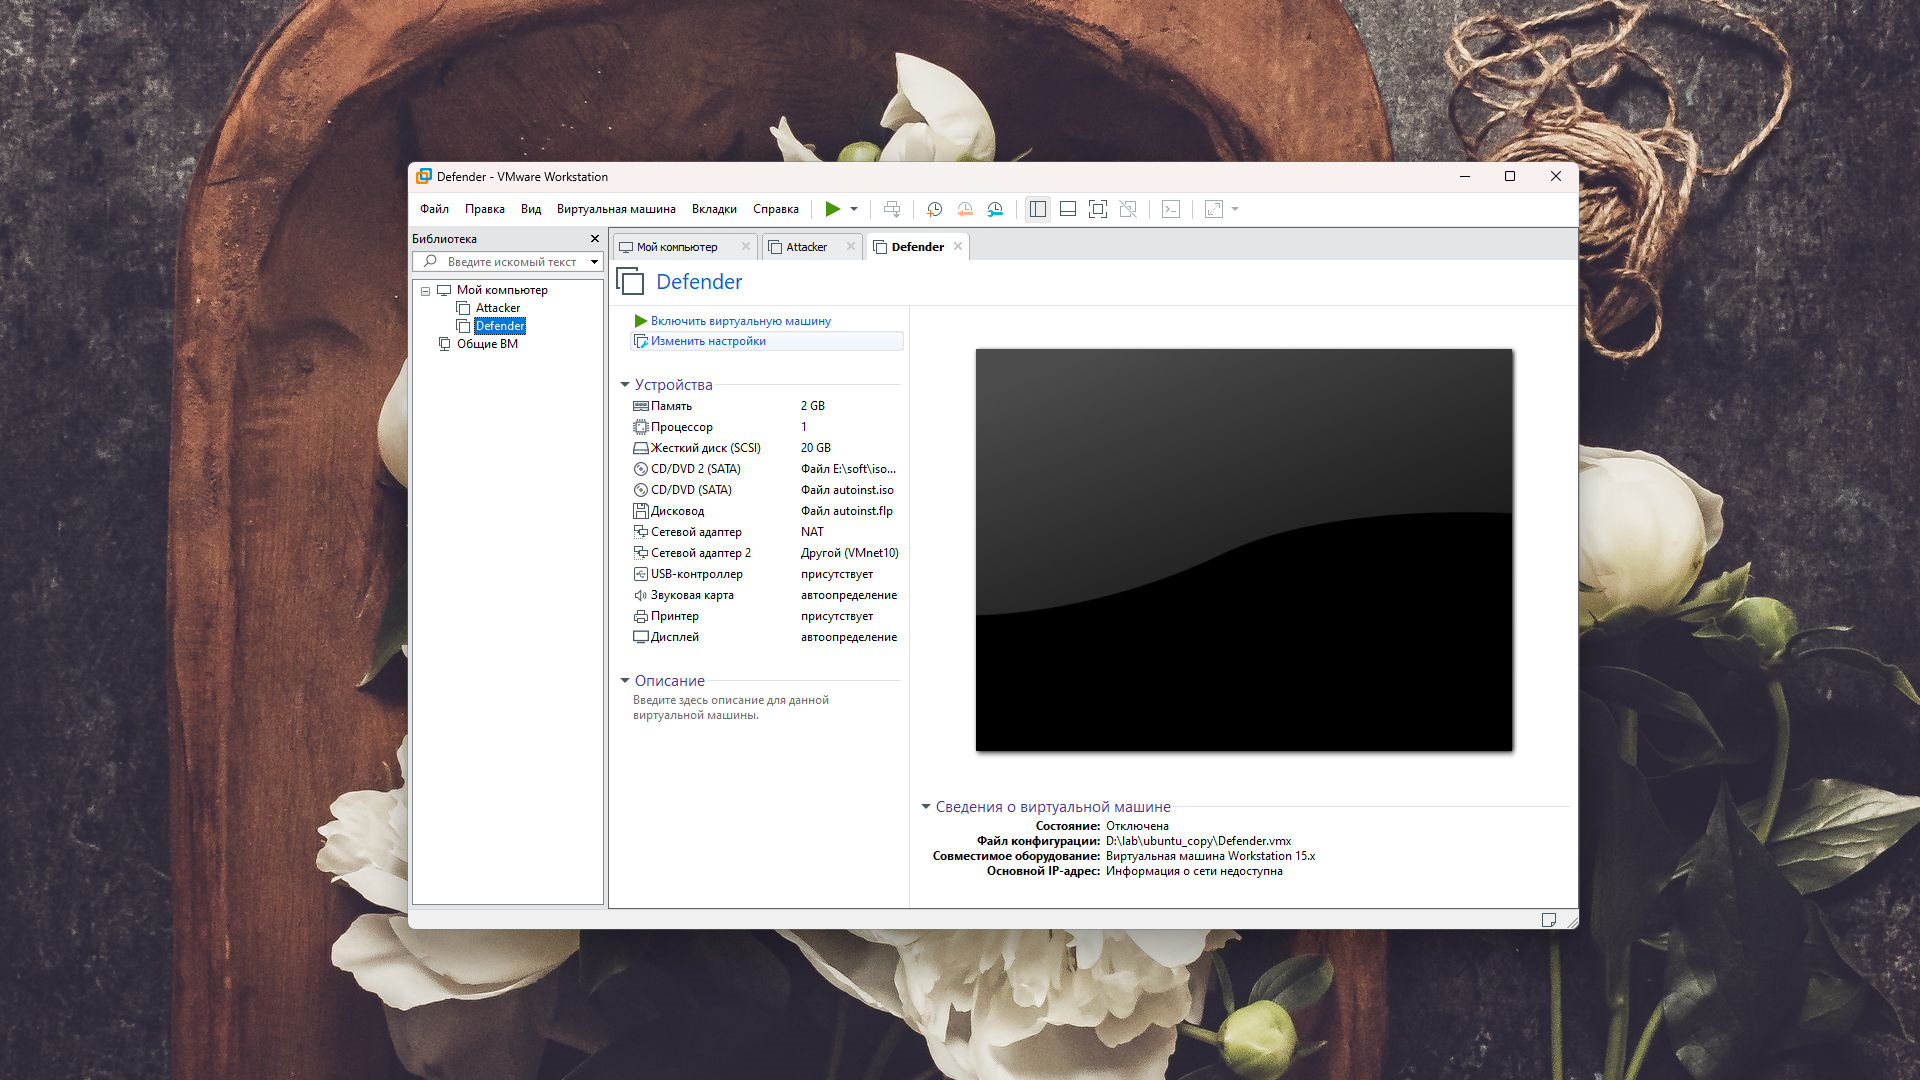
\includegraphics[width=0.85\textwidth]{03_00 (20)}
    \caption{Готовая атакуемая машина}
    \label{img:20}
  \end{figure}

  Теперь включим обе машины и зайдем на каждой из них в учетную запись пользователя \textit{user}:

  \begin{figure}[H]
    \centering
    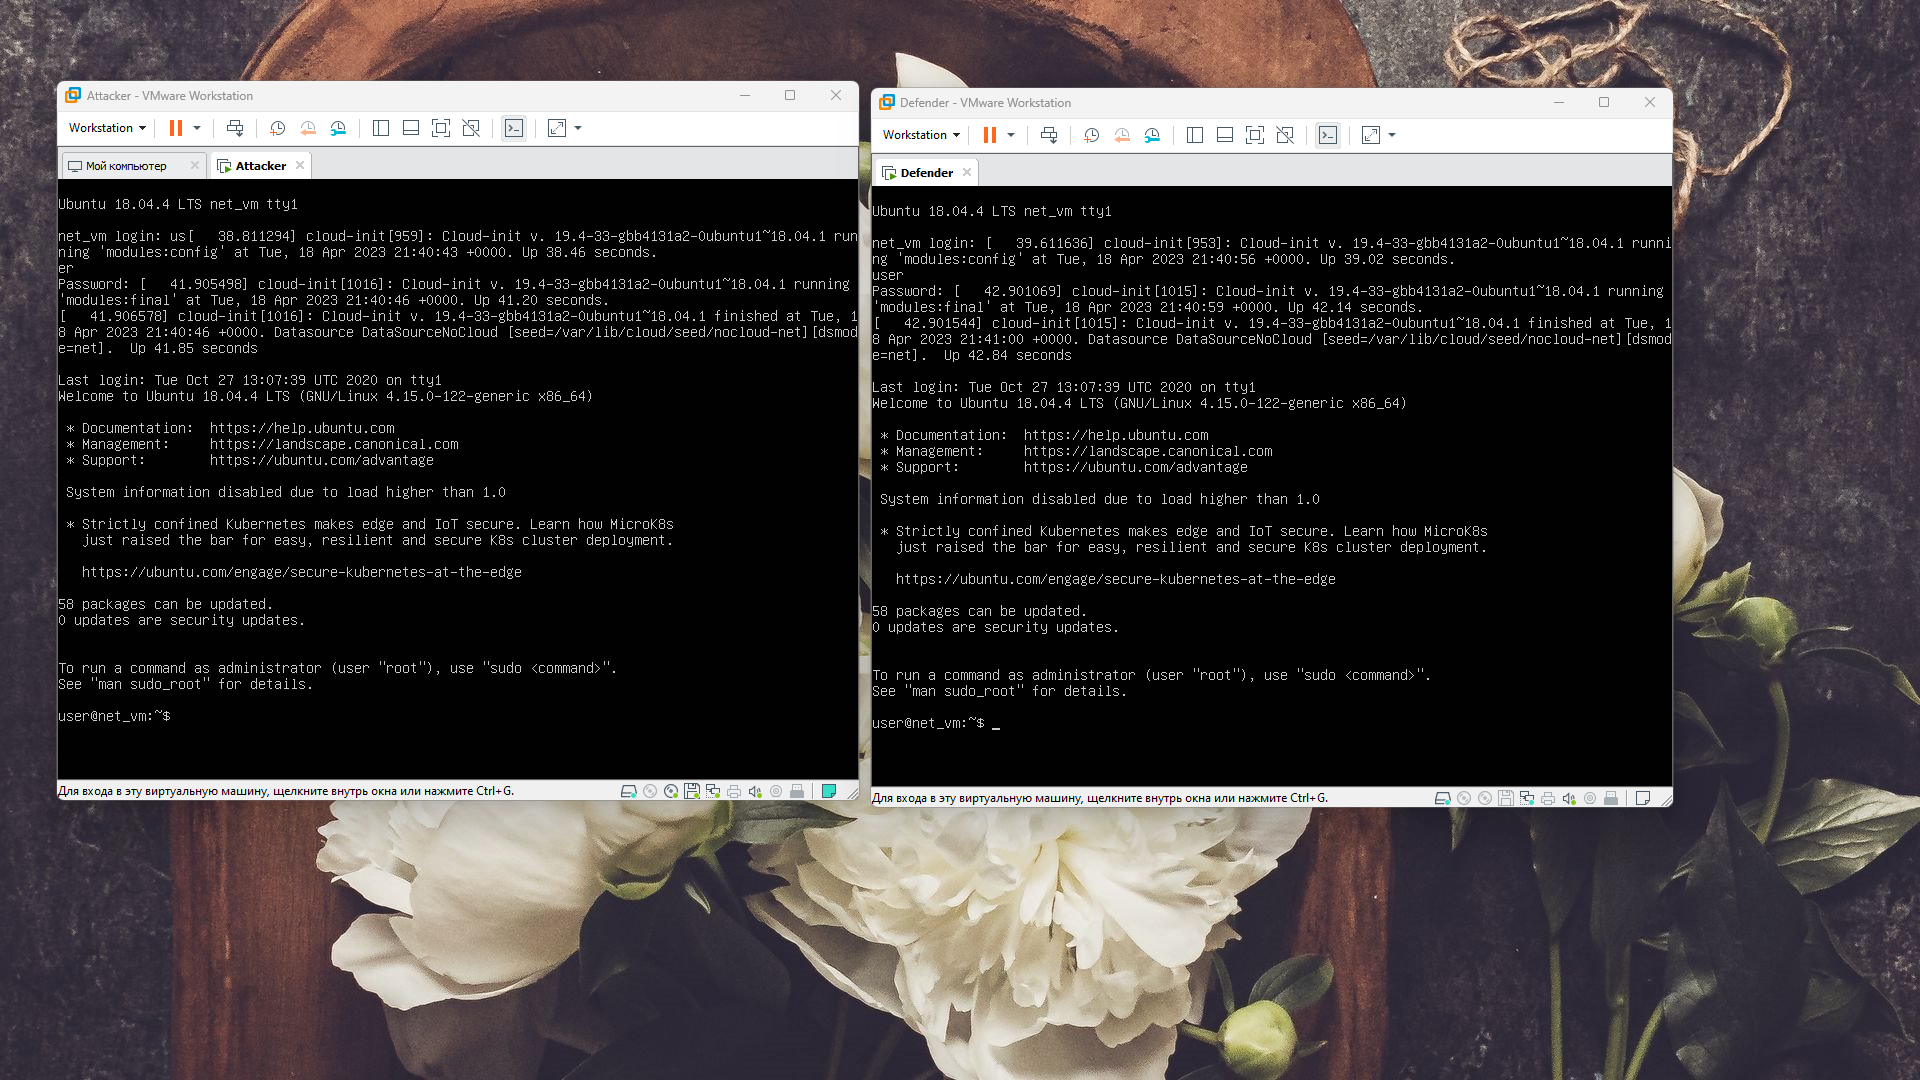
\includegraphics[width=0.85\textwidth]{03_00 (22)}
    \caption{Запущенные машины}
    \label{img:22}
  \end{figure}

  \subsubsection{Настройка пакетов}

  Теперь необходимо узнать сетевые параметры каждой из машины,
  для этого воспользуемся утилитой \textit{ip}:

  \begin{figure}[H]
    \centering
    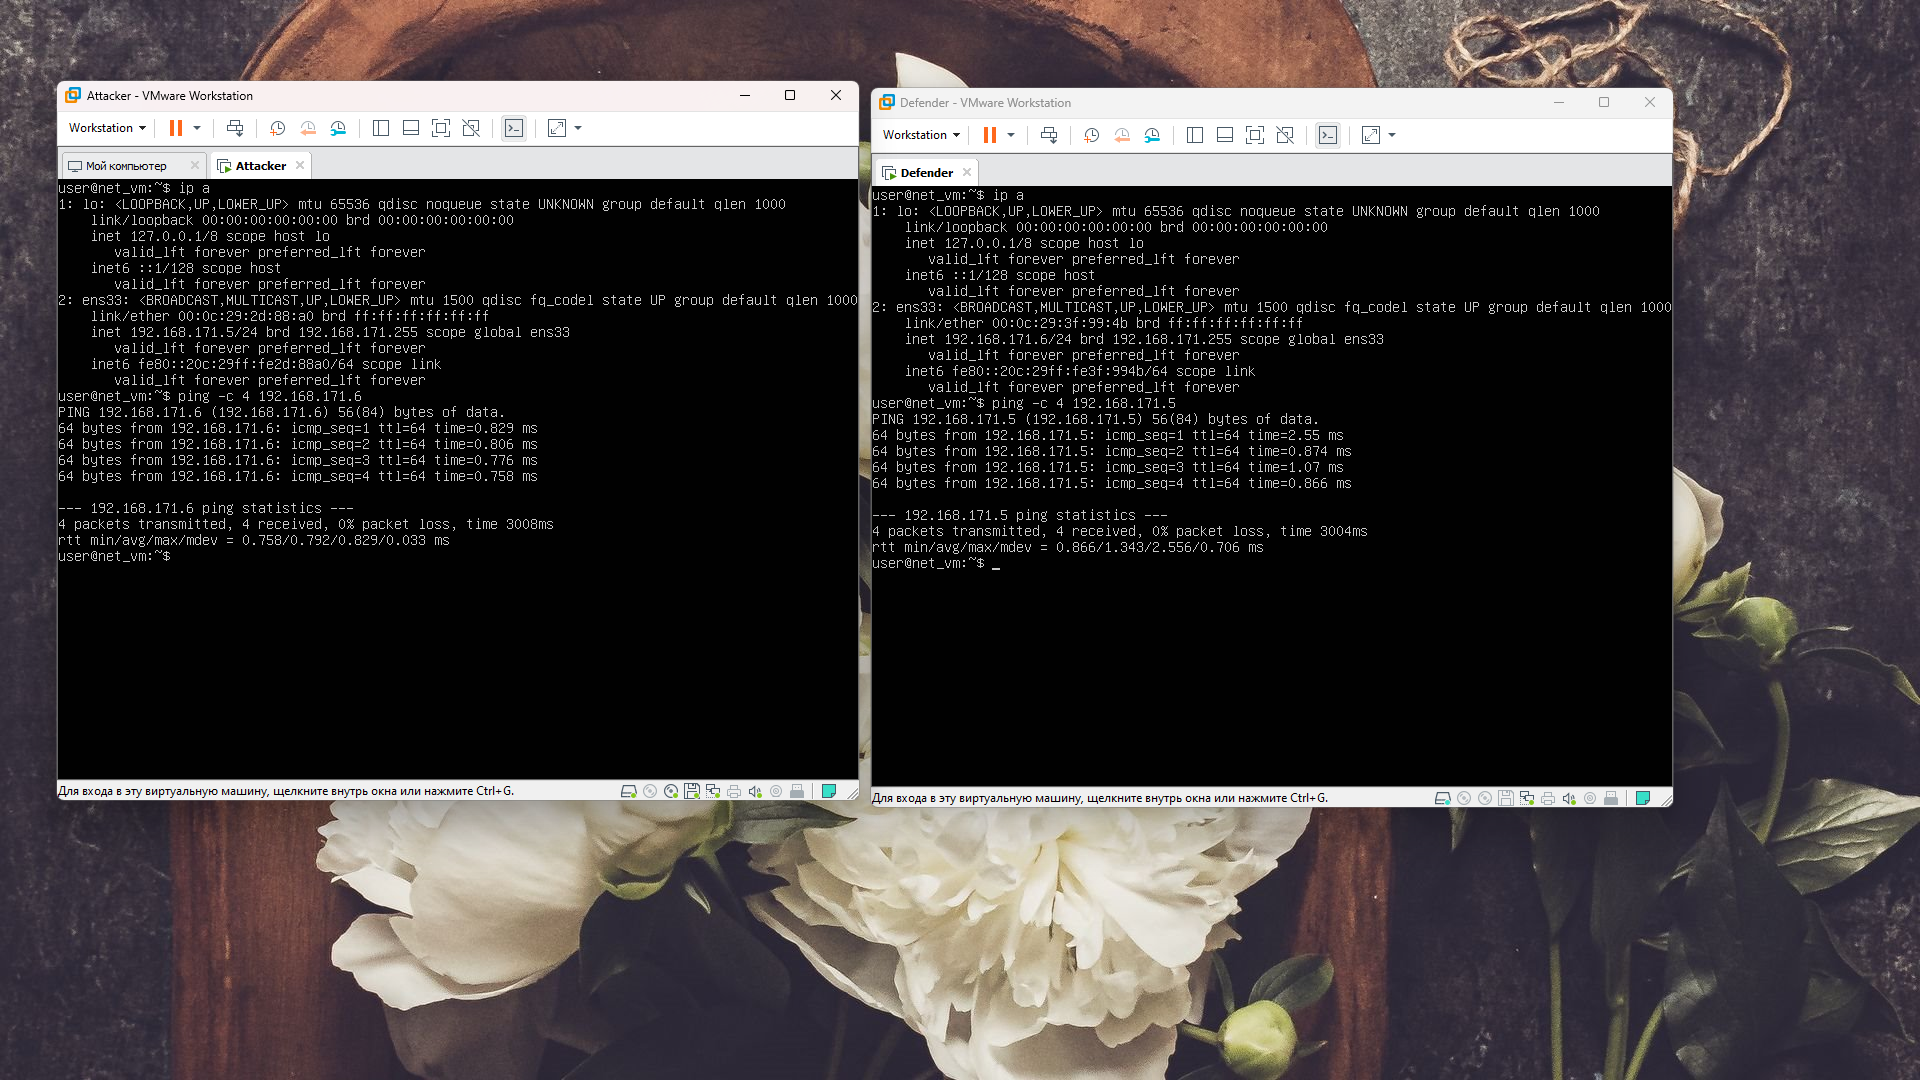
\includegraphics[width=0.85\textwidth]{03_00 (29)}
    \caption{\textit{ip a} - информация о сетевых интерфейсах устройства}
    \label{img:29}
  \end{figure}

  Вынесем полученные данные в таблицу:
  \begin{table}[H]
    \centering
    \begin{tabular}{| c | c | c |}
      \hline
      Имя машины & \textit{MAC} адрес & \textit{IPv4} адрес \\
      \hline
      Attacker & 00:0C:29:2d:88:A0 & 192.168.171.5 \\
      \hline
      Defender & 00:0C:29:3F:99:4B & 192.168.171.6 \\
      \hline
    \end{tabular}
  \end{table}

  Также на изображении представлен результат перекрустного пинга,
  подтверждающий, что машины действительно находятся в одной сети
  и могут создавать подключение между друг другом.

  Теперь необходимо обновить машины, для этого сначала загрузим свежие
  списки пакетов, а затем скачаем и установим новые версии для устревших.
  Сделать это можно при помощи утилиты \textit{apt}:

  \begin{minted}{bash}
    sudo apt update  # Обновление списков пакетов
    sudo apt upgrade # Само обновление пакетов
  \end{minted}

  \begin{figure}[H]
    \centering
    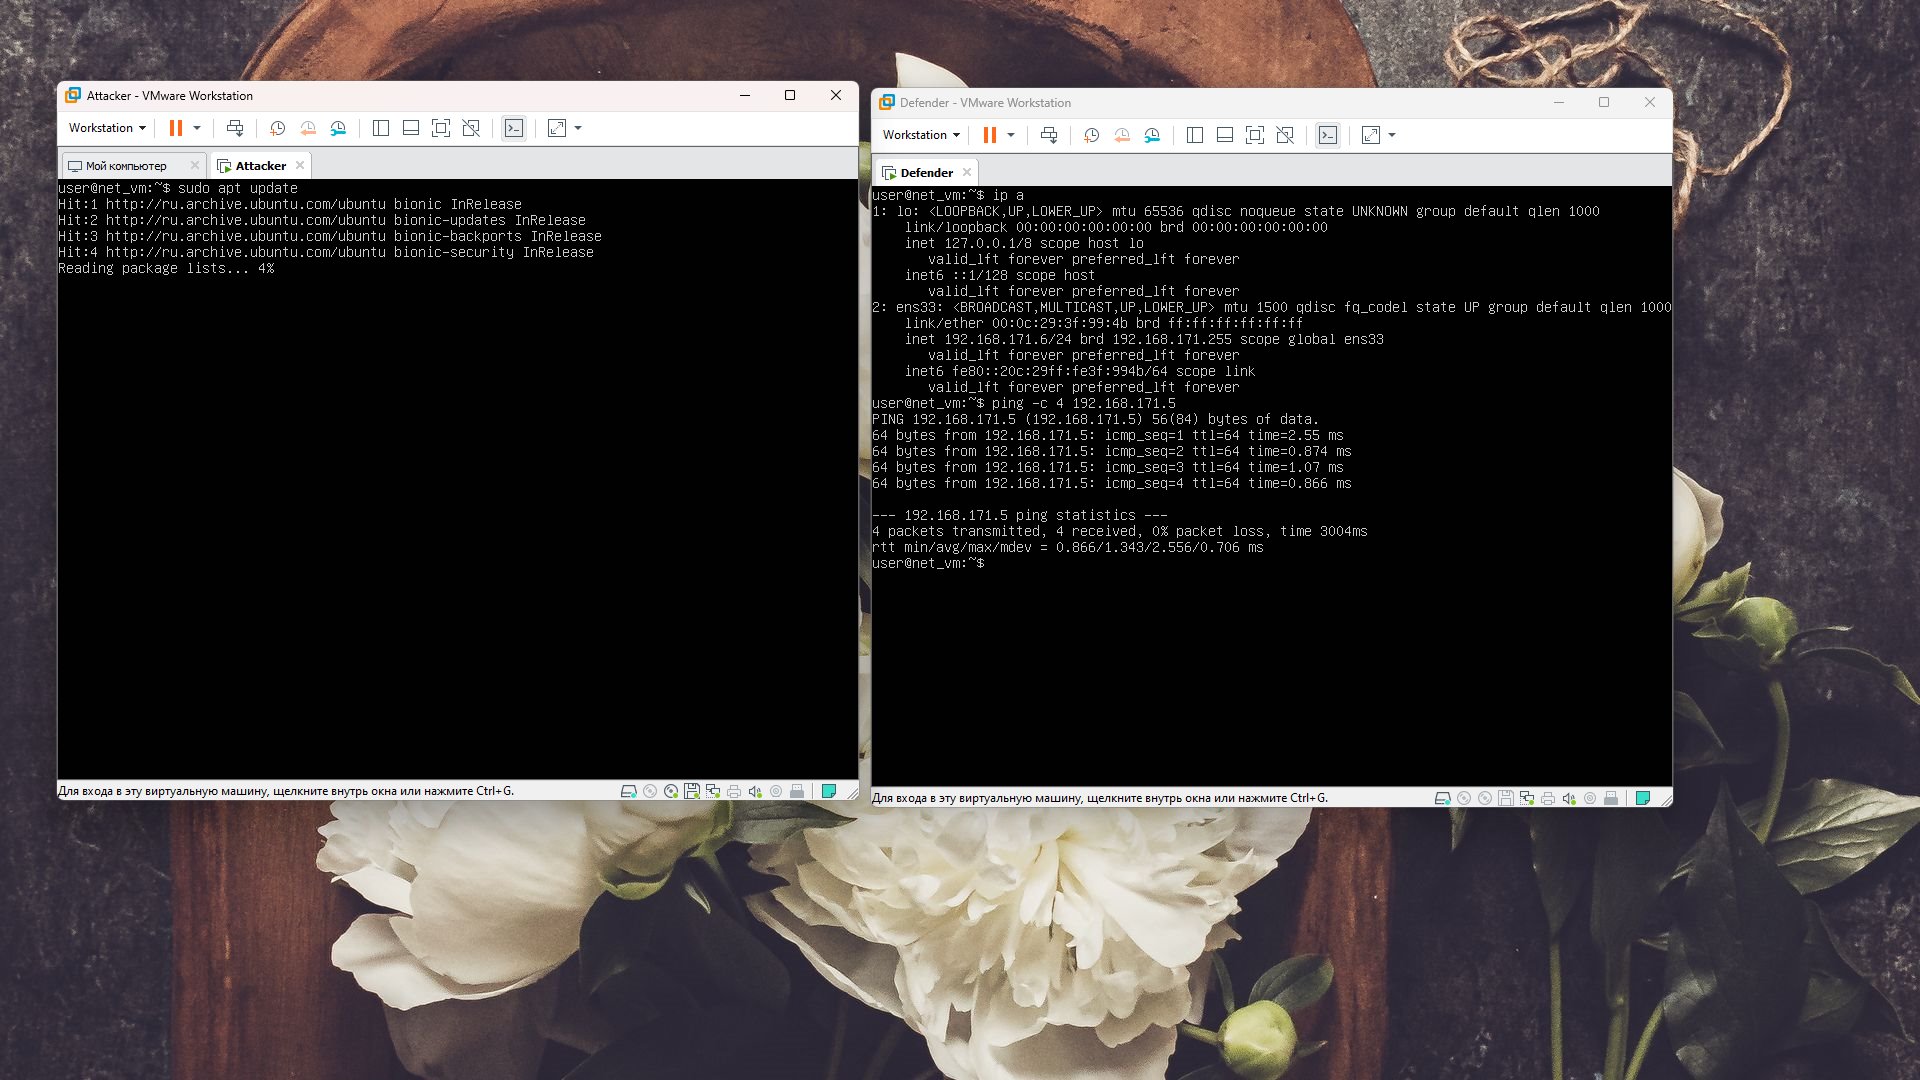
\includegraphics[width=0.85\textwidth]{03_00 (30)}
    \caption{\textit{apt update} на атакующей машине}
    \label{img:30}
  \end{figure}

  \begin{figure}[H]
    \centering
    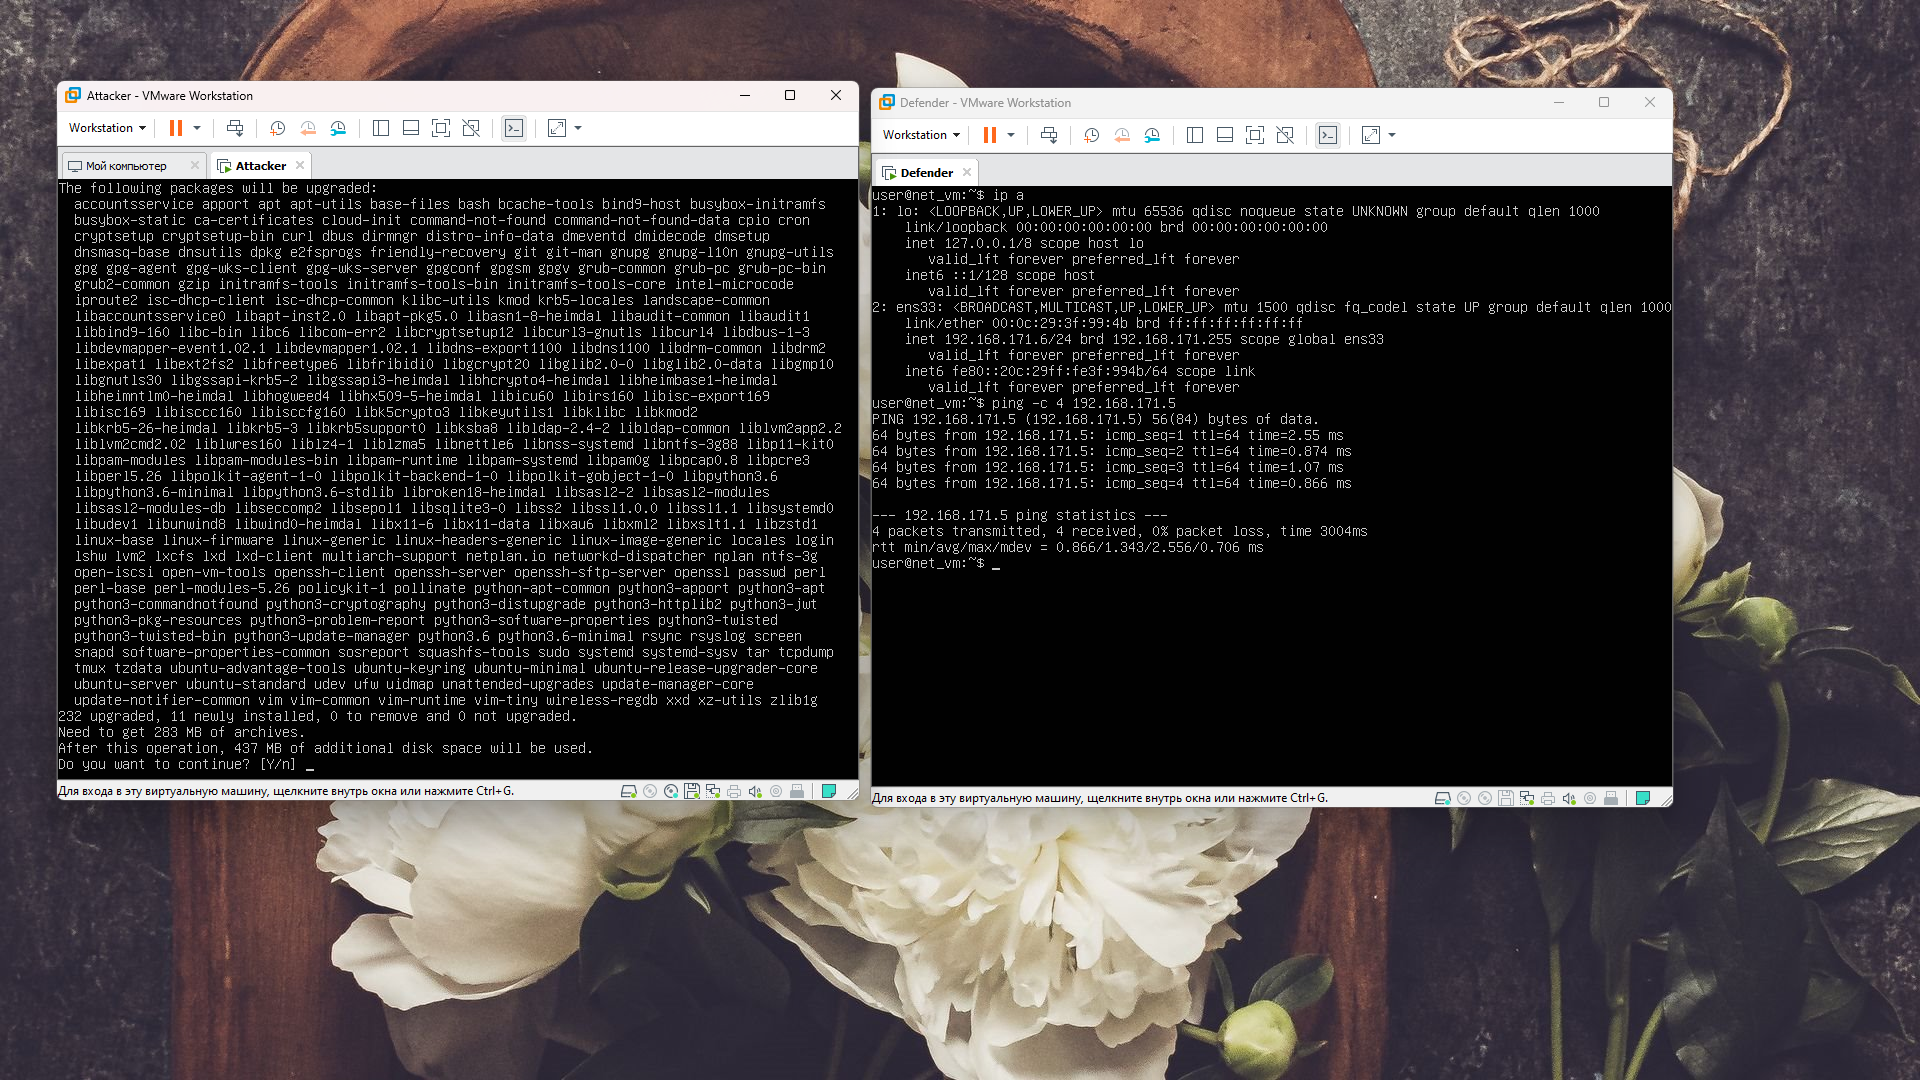
\includegraphics[width=0.85\textwidth]{03_00 (31)}
    \caption{\textit{apt upgrade} на атакующей машине}
    \label{img:31}
  \end{figure}

  Такие же команды были выполнены и на атакуемой машине (можно видеть результат
  их работы на следующих скриншотах).

  Для выполнения работы также потребуются некоторые утилиты: для атакующей машины \textit{curl}
  и \textit{nmap}, а для атакуемой - \textit{apache2} (web сервер). Загрузить их можно
  при помощи того же \textit{apt}:

  \begin{figure}[H]
    \centering
    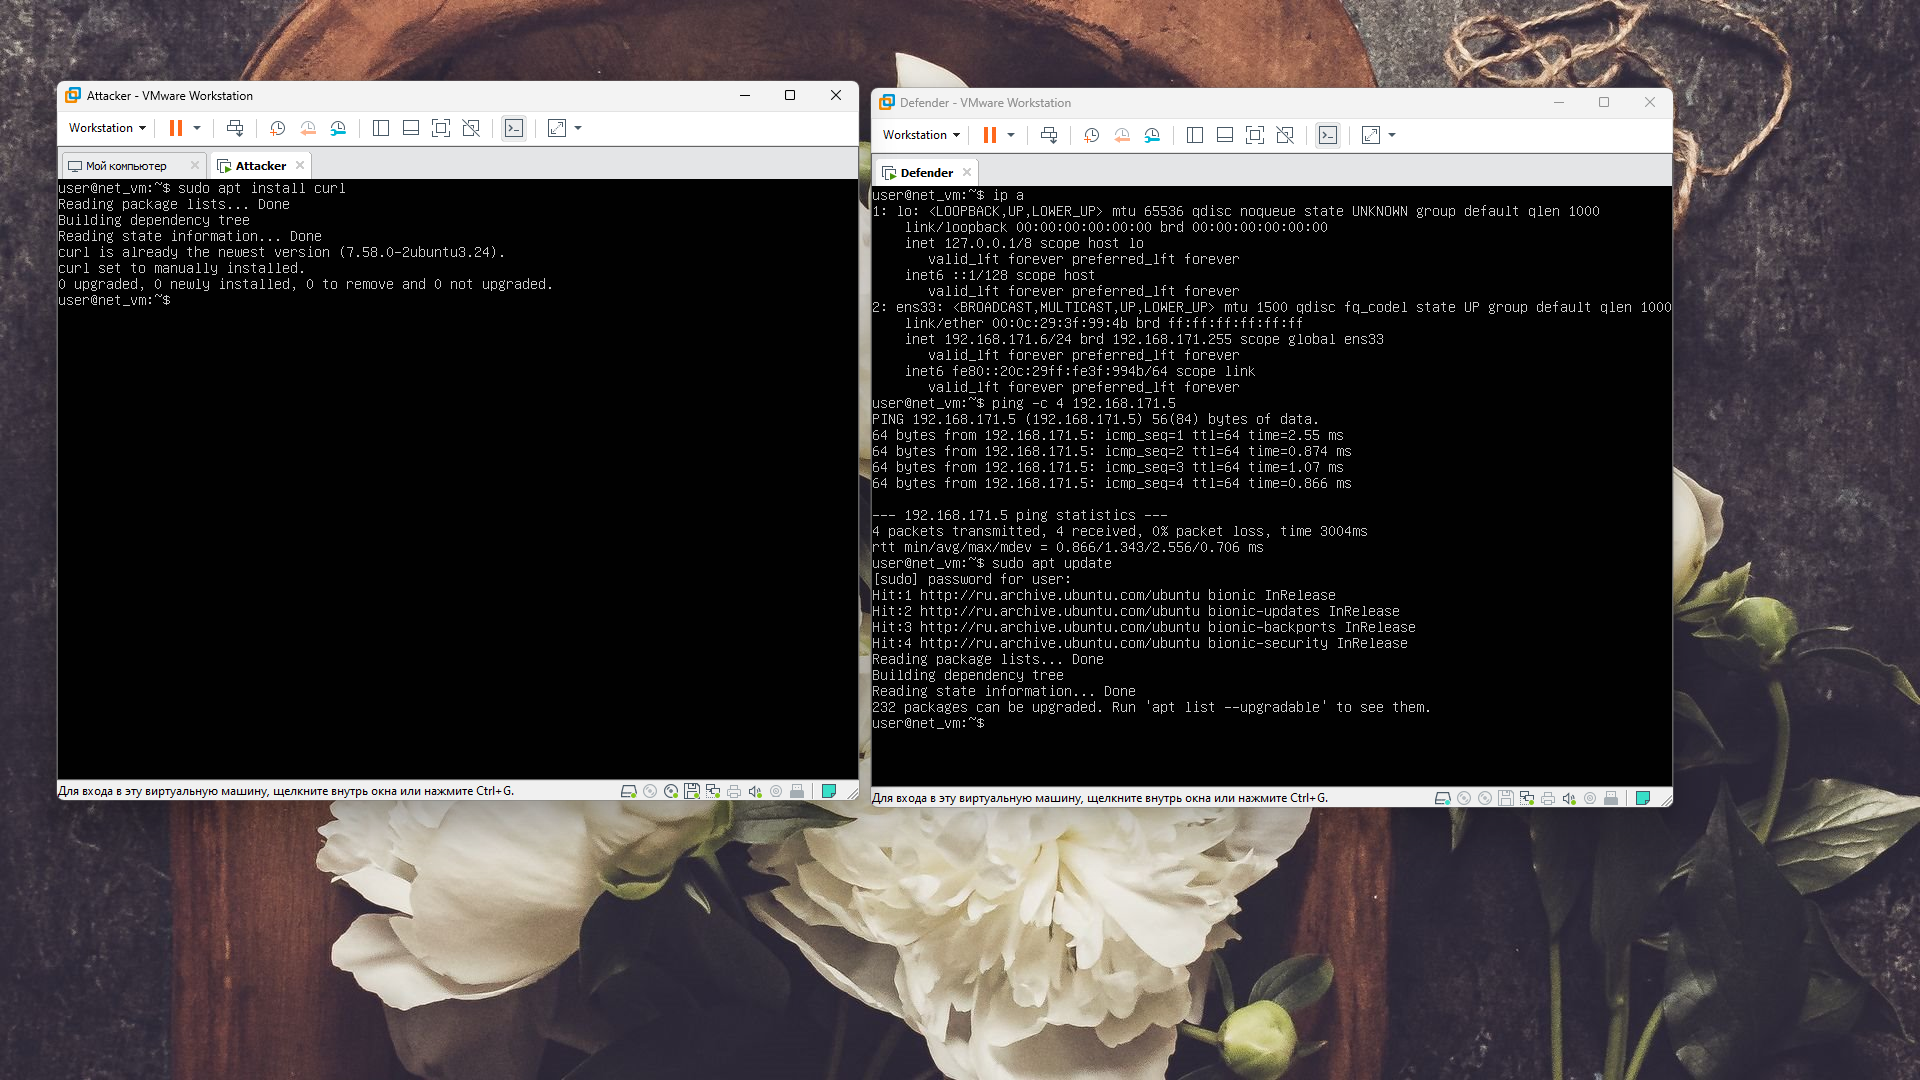
\includegraphics[width=0.85\textwidth]{03_00 (33)}
    \caption{\textit{apt install curl} - загрузка и установка \textit{curl}}
    \label{img:33}
  \end{figure}

  \begin{figure}[H]
    \centering
    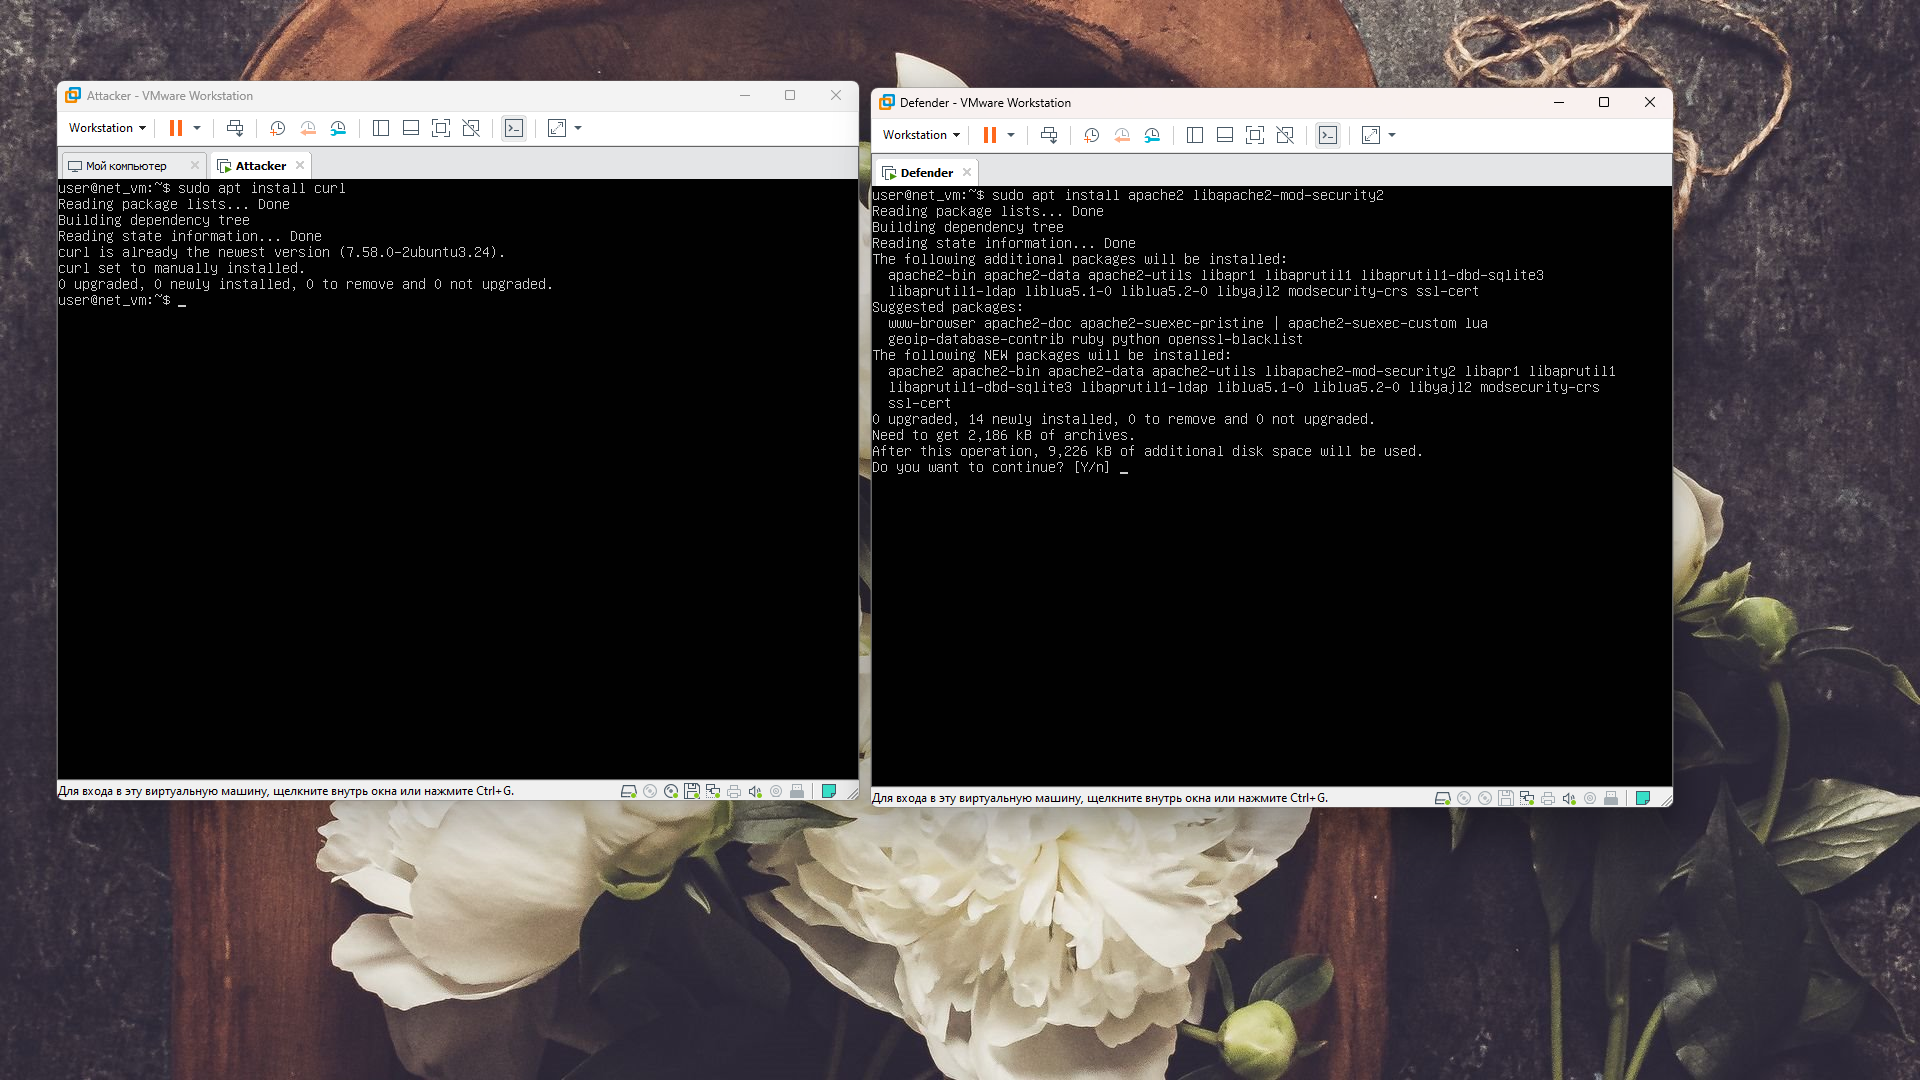
\includegraphics[width=0.85\textwidth]{03_00 (35)}
    \caption{\textit{apt install apache2 libapache2-mod-security2} - загрузка и установка \textit{apache2} и дополнительного модуля безопасности для него}
    \label{img:35}
  \end{figure}

  Вместе с \textit{web}-сервером также был загружен дополнительный модуль, который
  в будущем позволить фильтровать запросы. Для того, чтобы удостовериться, что он определился
  в системе, воспользуемся \textit{apachectl}:

  \begin{figure}[H]
    \centering
    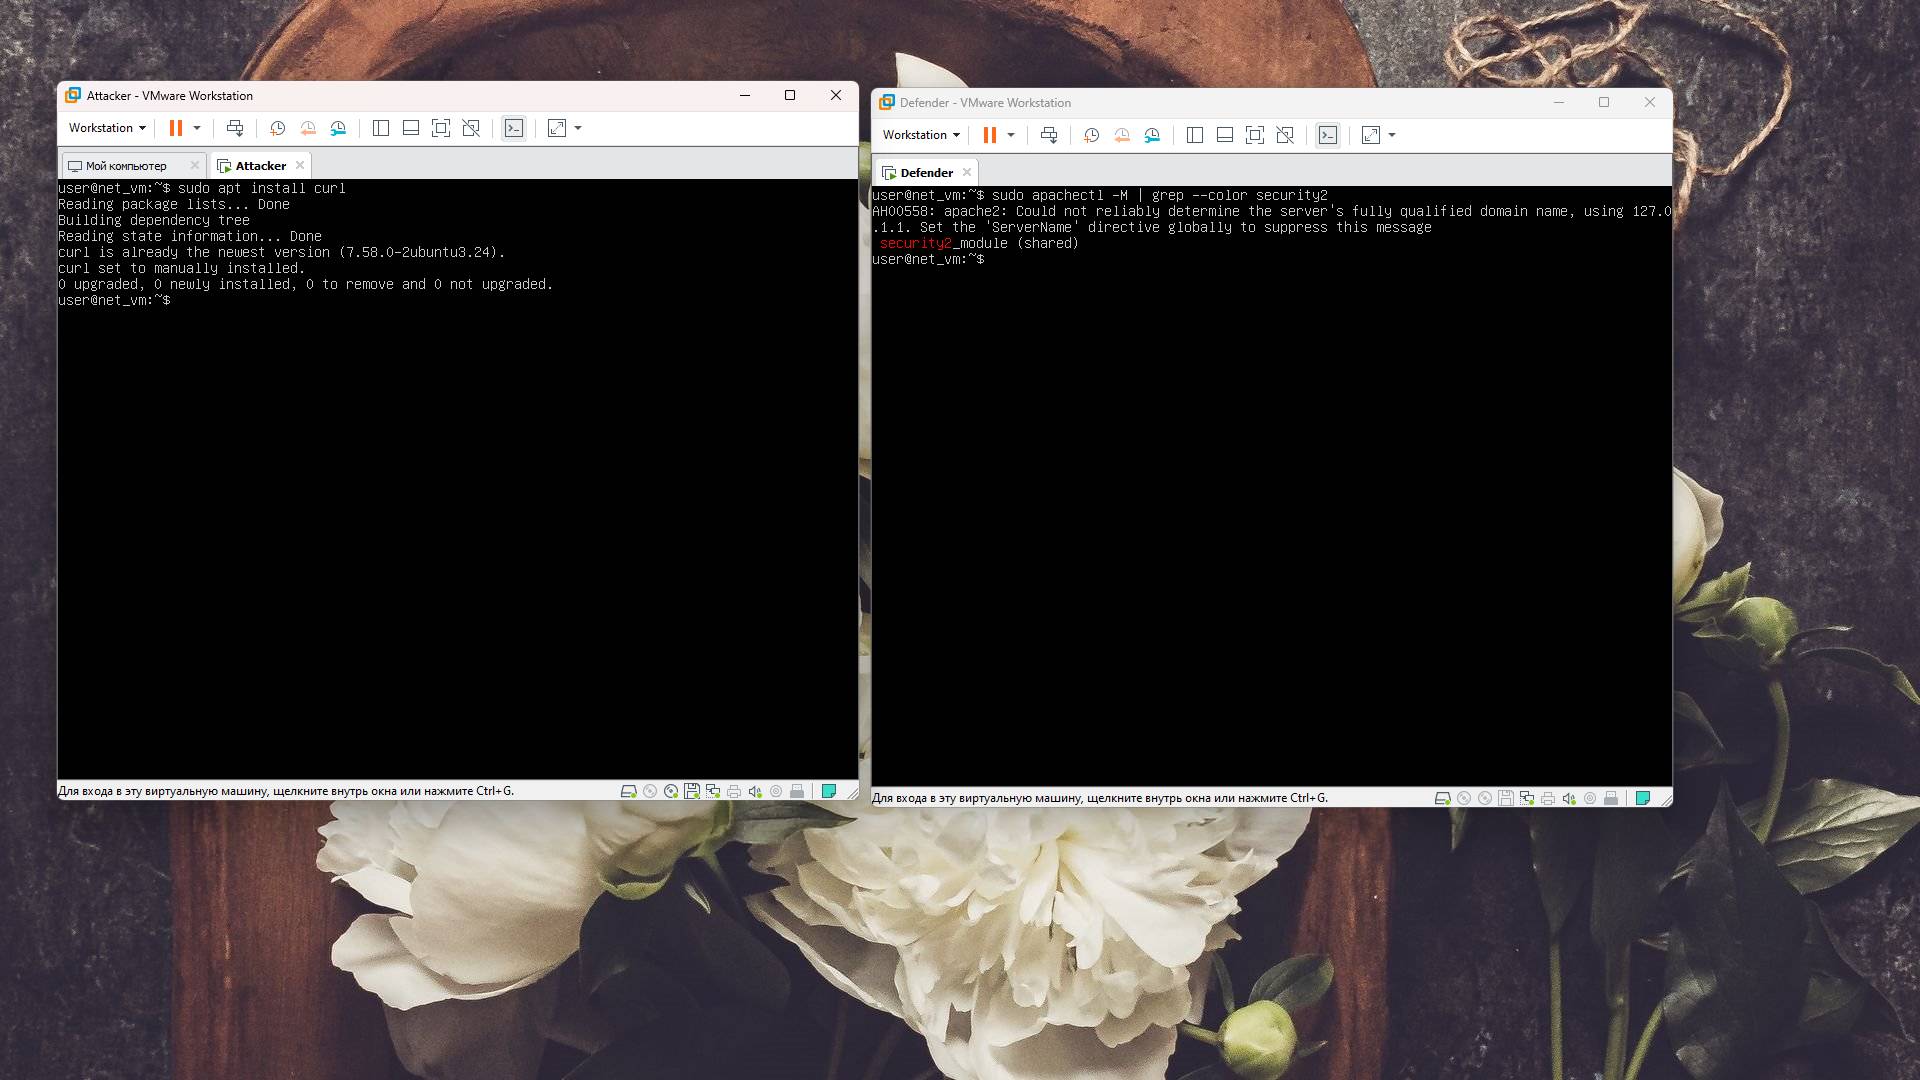
\includegraphics[width=0.85\textwidth]{03_00 (36)}
    \caption{Видно, что модуль безопасности действительно установлен}
    \label{img:36}
  \end{figure}

  \begin{figure}[H]
    \centering
    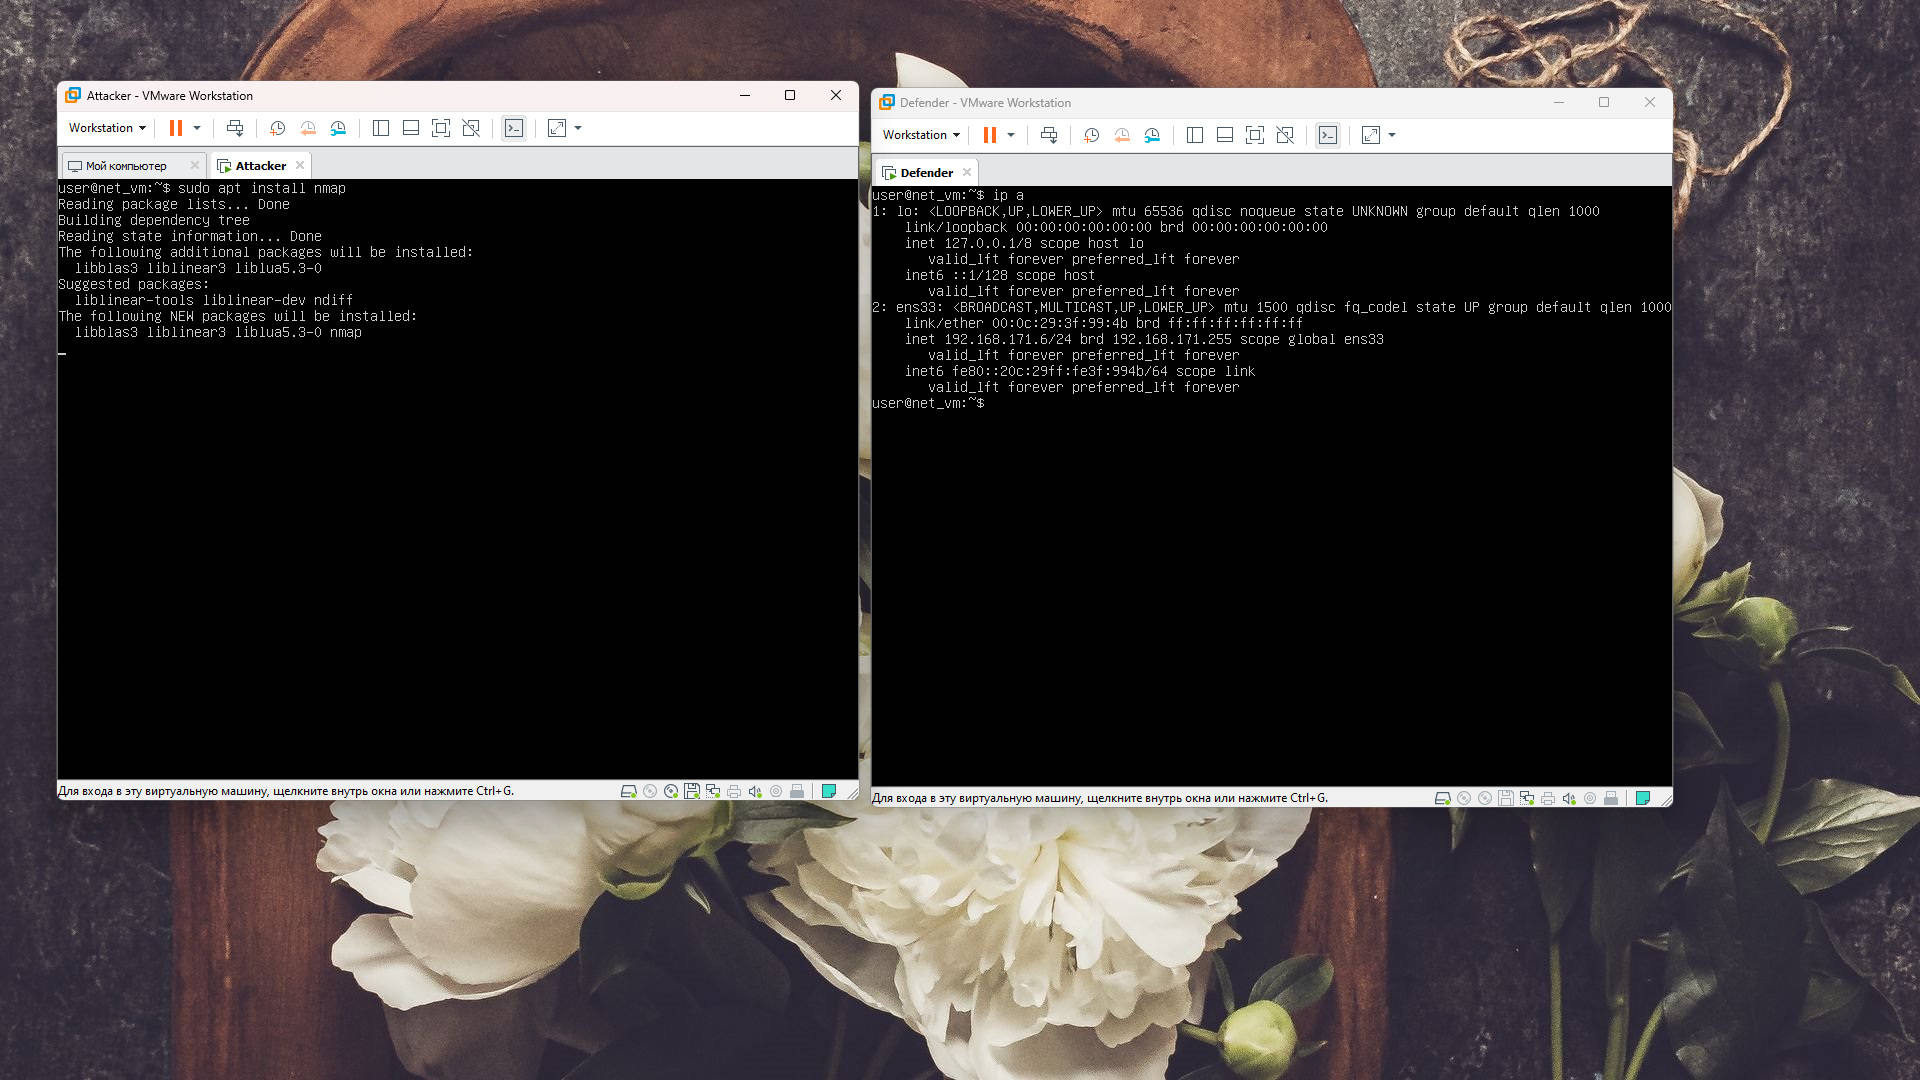
\includegraphics[width=0.85\textwidth]{03_00 (37)}
    \caption{\textit{apt install nmap} - установка \textit{nmap}}
    \label{img:37}
  \end{figure}

  Теперь все необходимые пакеты скачаны, попробуем провести \textit{XMas} сканирование
  атакуюемой машины при помощи \textit{nmap}:

  \begin{figure}[H]
    \centering
    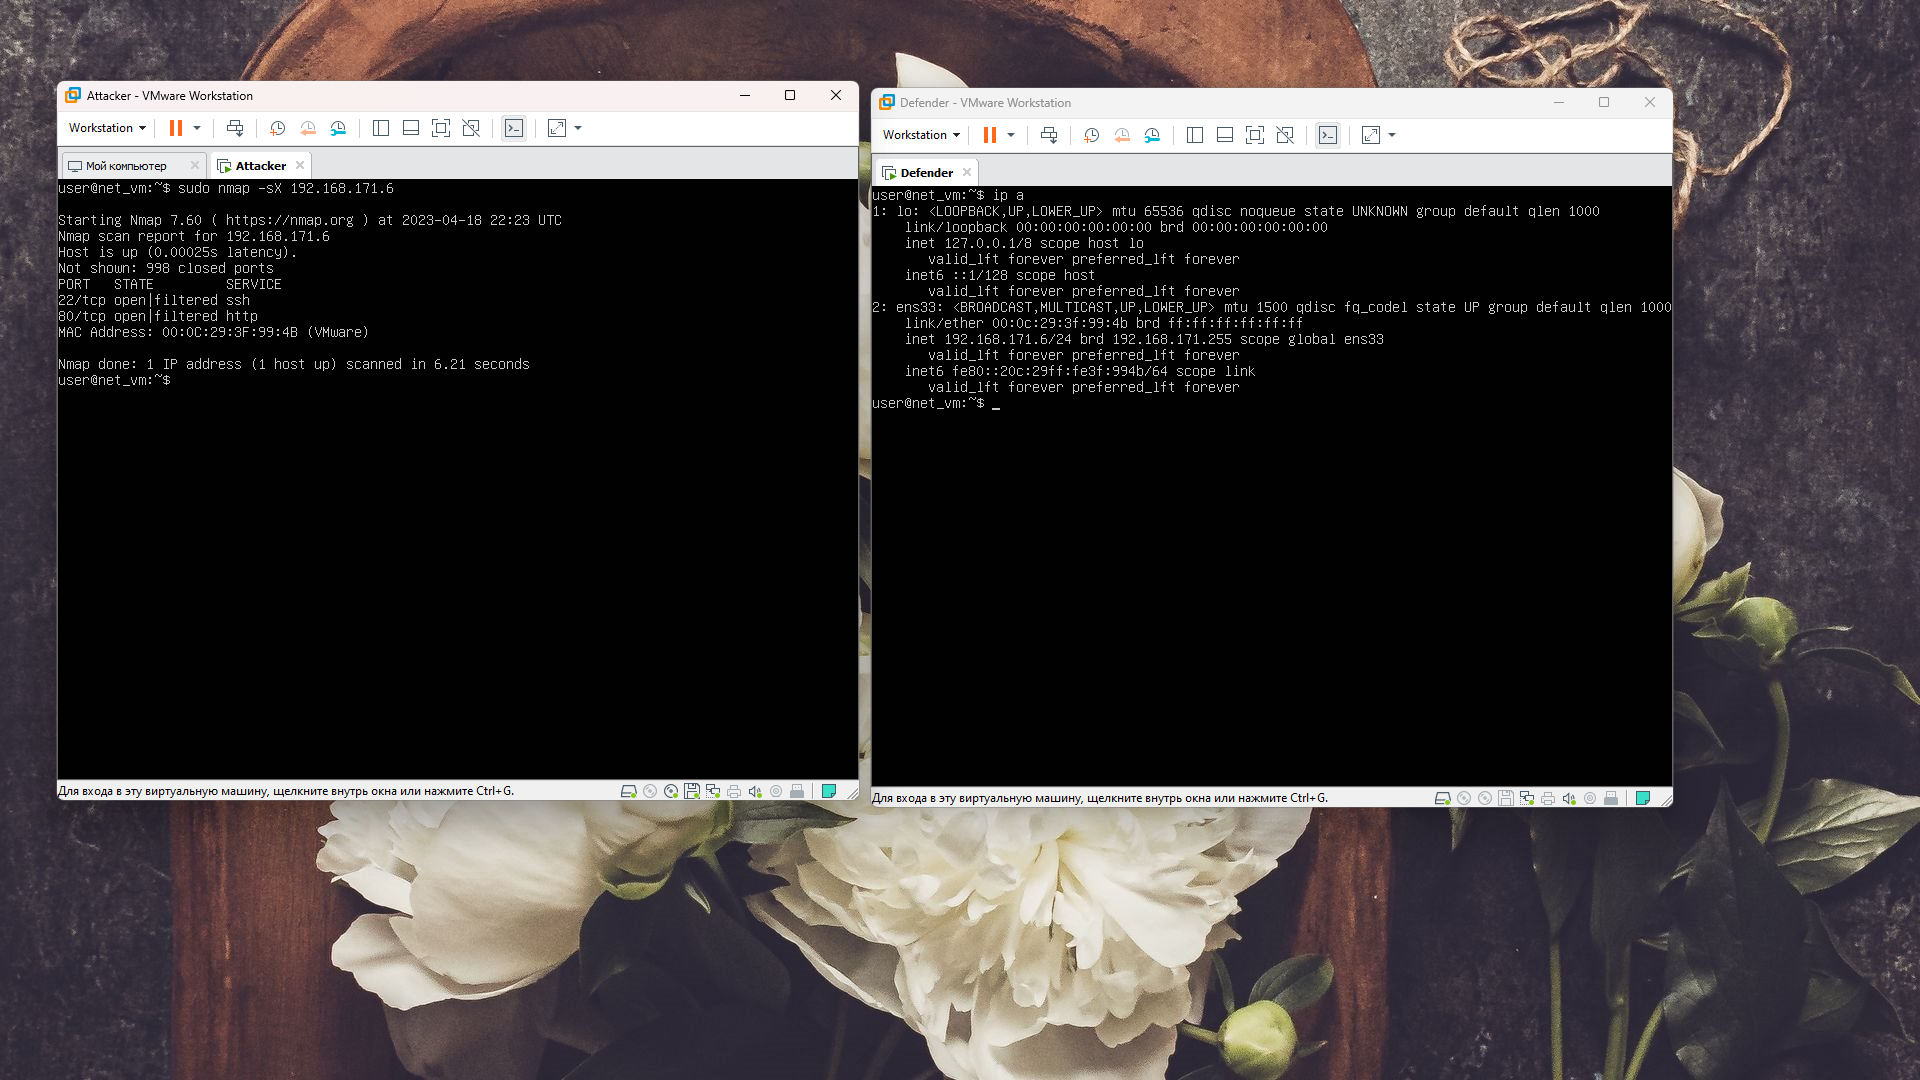
\includegraphics[width=0.85\textwidth]{03_00 (38)}
    \caption{\textit{nmap -xS 192.168.171.6} - \textit{XMas} сканирование}
    \label{img:38}
  \end{figure}

  По результатам сканирования видно, что на атакуемой машине открыты два порта - 22 для ssh
  и 80 для http соединений.

  \subsection{Настройка iptables}

  \textit{iptables} - утилита, предназначенная для настройки сетевого экрана, по умолчанию
  установлена в системы, поэтому для начала рассмотрим стандартную политику:

  \begin{figure}[H]
    \centering
    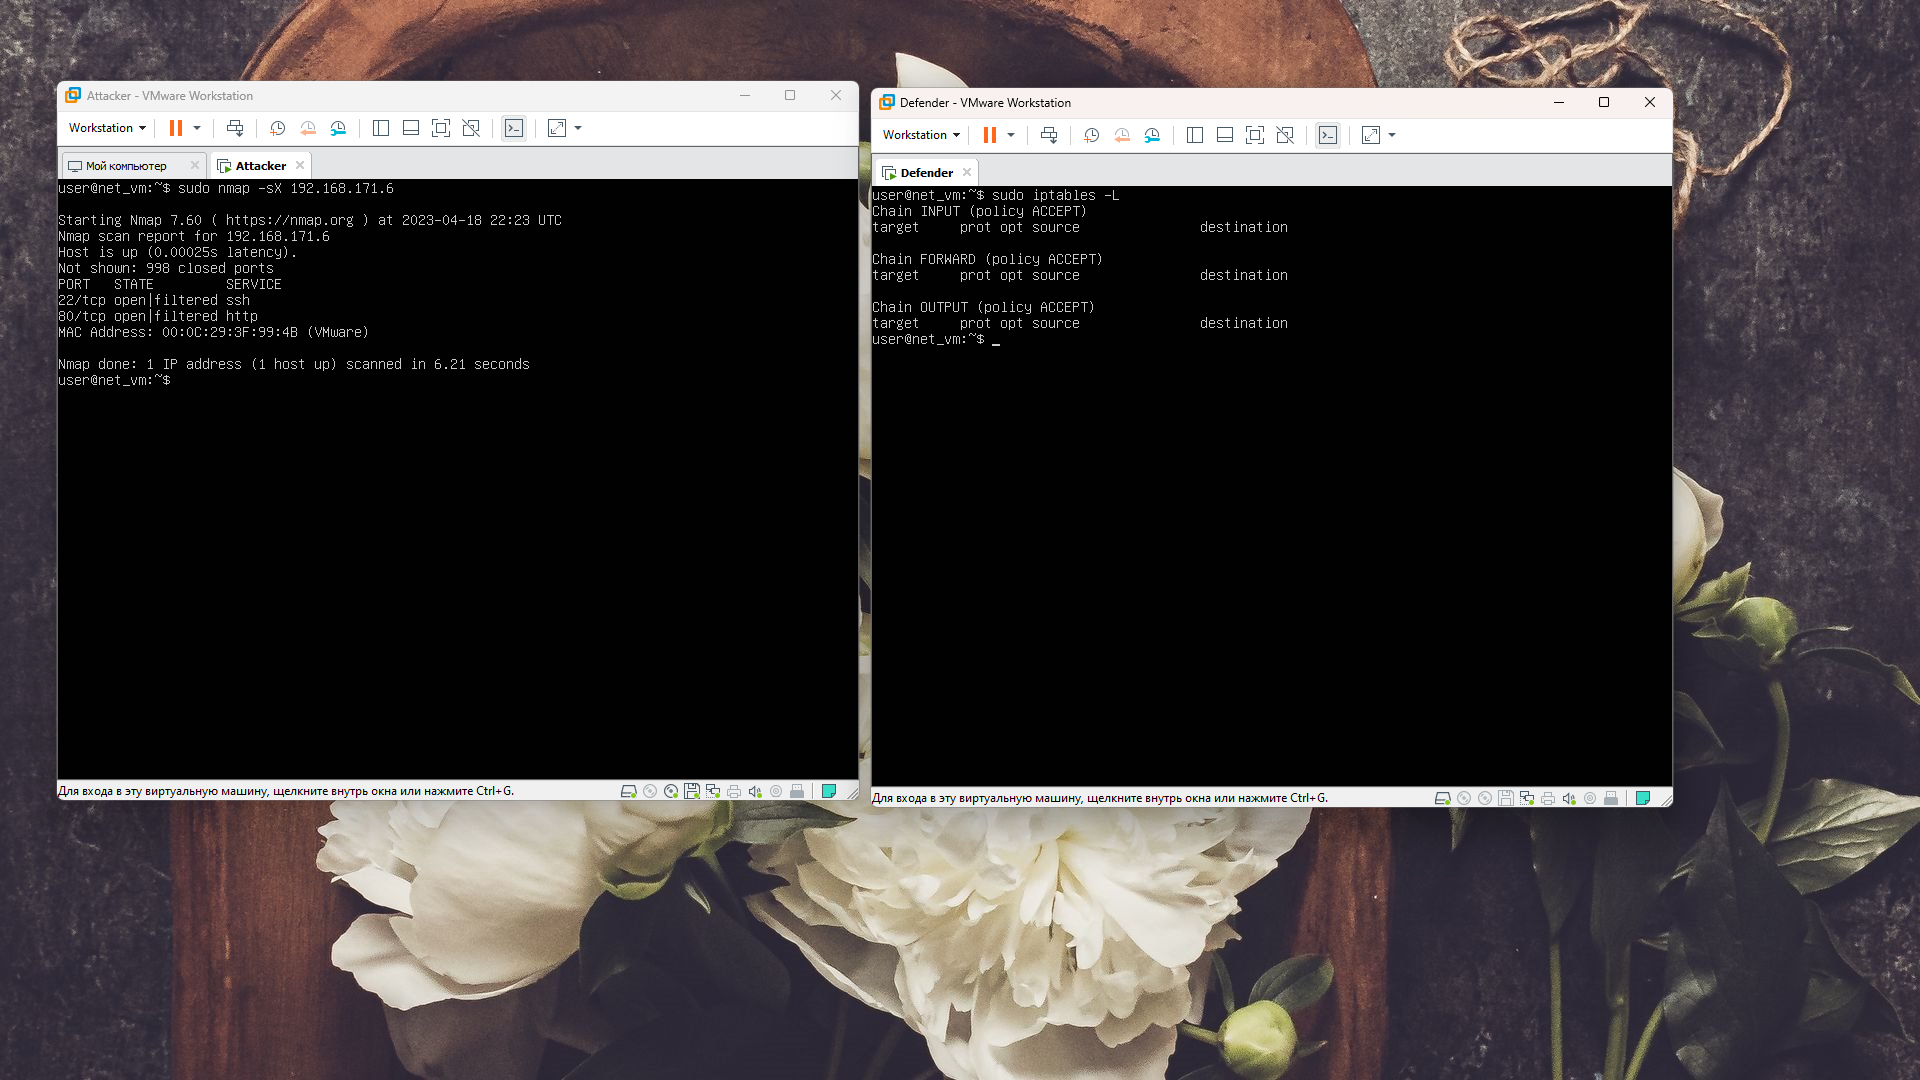
\includegraphics[width=0.85\textwidth]{03_00 (39)}
    \caption{\textit{iptables -L} - посмотреть существующие правила}
    \label{img:39}
  \end{figure}

  \begin{figure}[H]
    \centering
    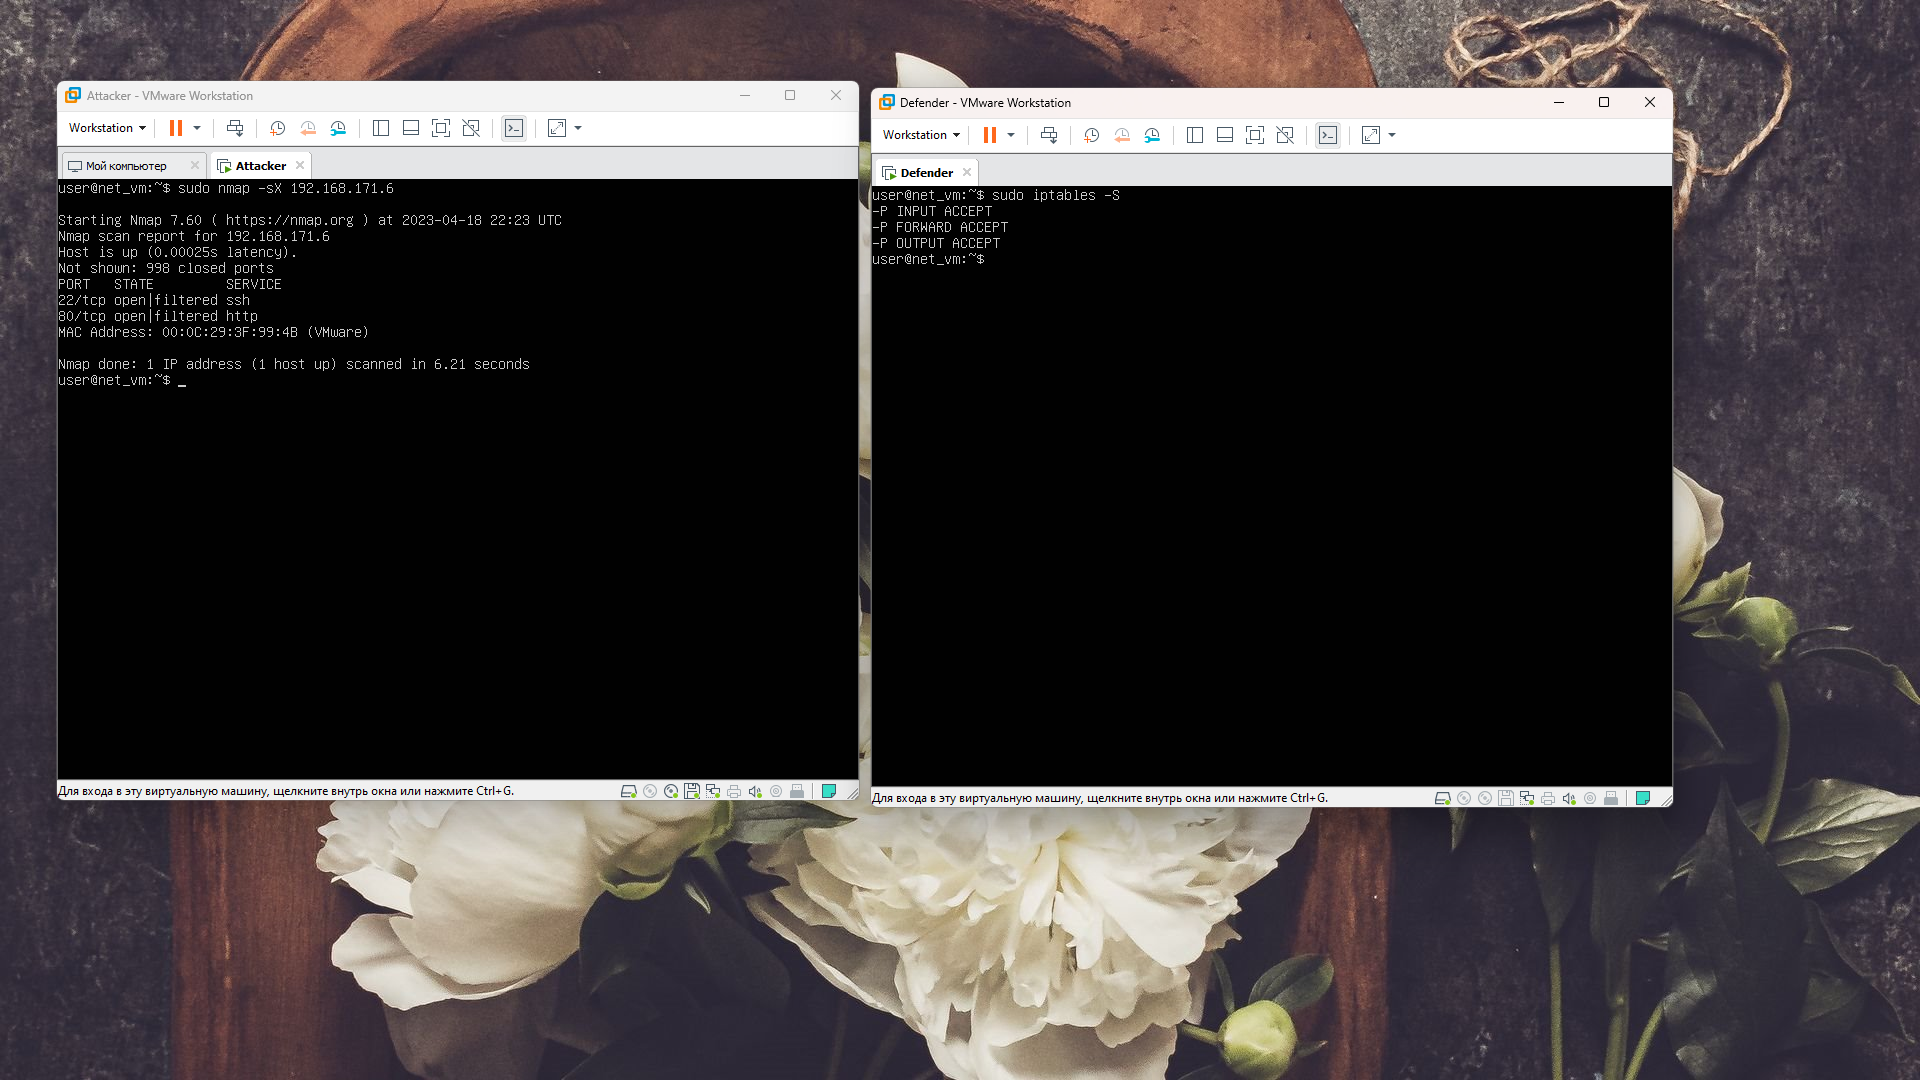
\includegraphics[width=0.85\textwidth]{03_00 (40)}
    \caption{\textit{iptables -S} - посмотреть существующие правила (альтернативный вариант)}
    \label{img:40}
  \end{figure}

  Исходя из вывода утилиты видно, что на атакуемой машине разрешены все входящие (INPUT), исходящие (OUTPUT)
  и проходящие (через нее, как посрденика) (FORWARD) соединения.

  Настроенные правила всегда можно сбросить при помощи флага \textit{-F}:

  \begin{figure}[H]
    \centering
    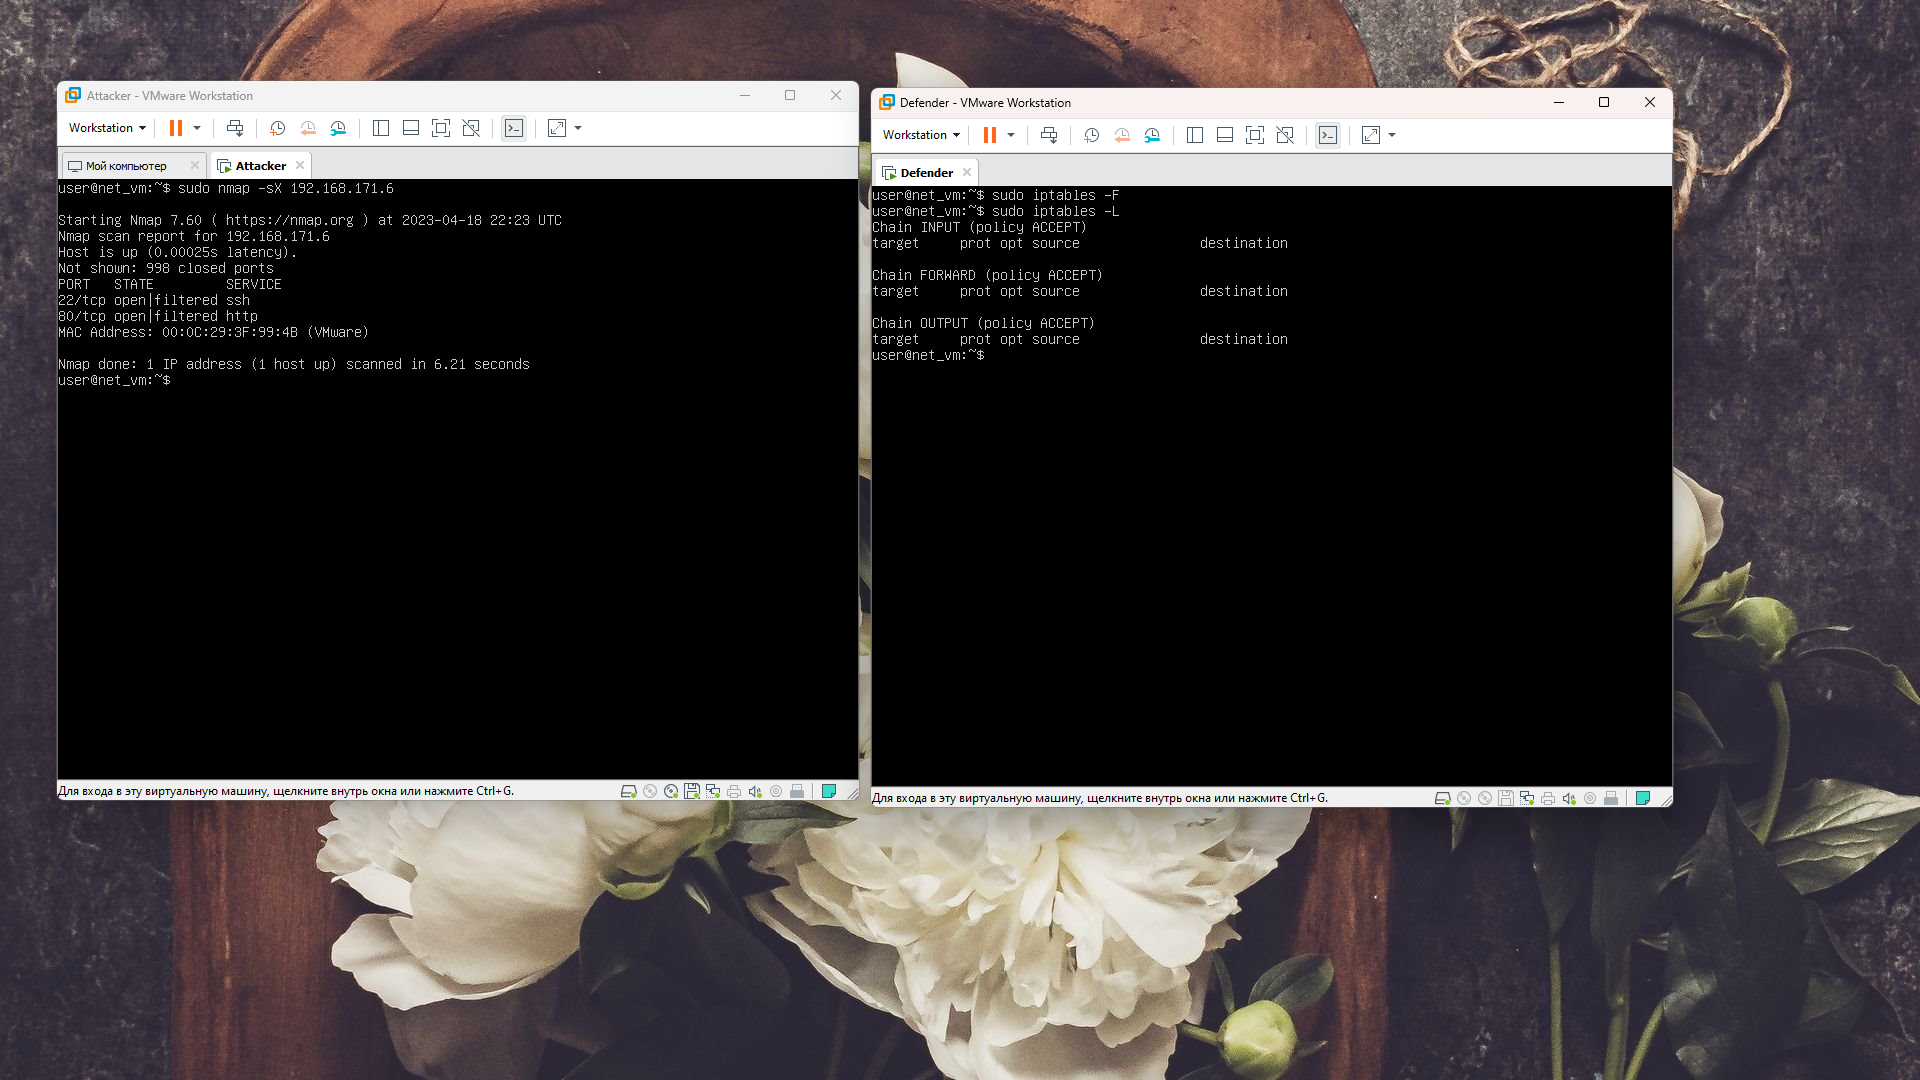
\includegraphics[width=0.85\textwidth]{03_00 (41)}
    \caption{Сброс дефолтных параметров к дефолтным}
    \label{img:41}
  \end{figure}

  Теперь добавим новое правило к цепочке INPUT - разрешим все входящие пакеты,
  приходящие на сетевой интерфейс \textit{lo}:

  \begin{figure}[H]
    \centering
    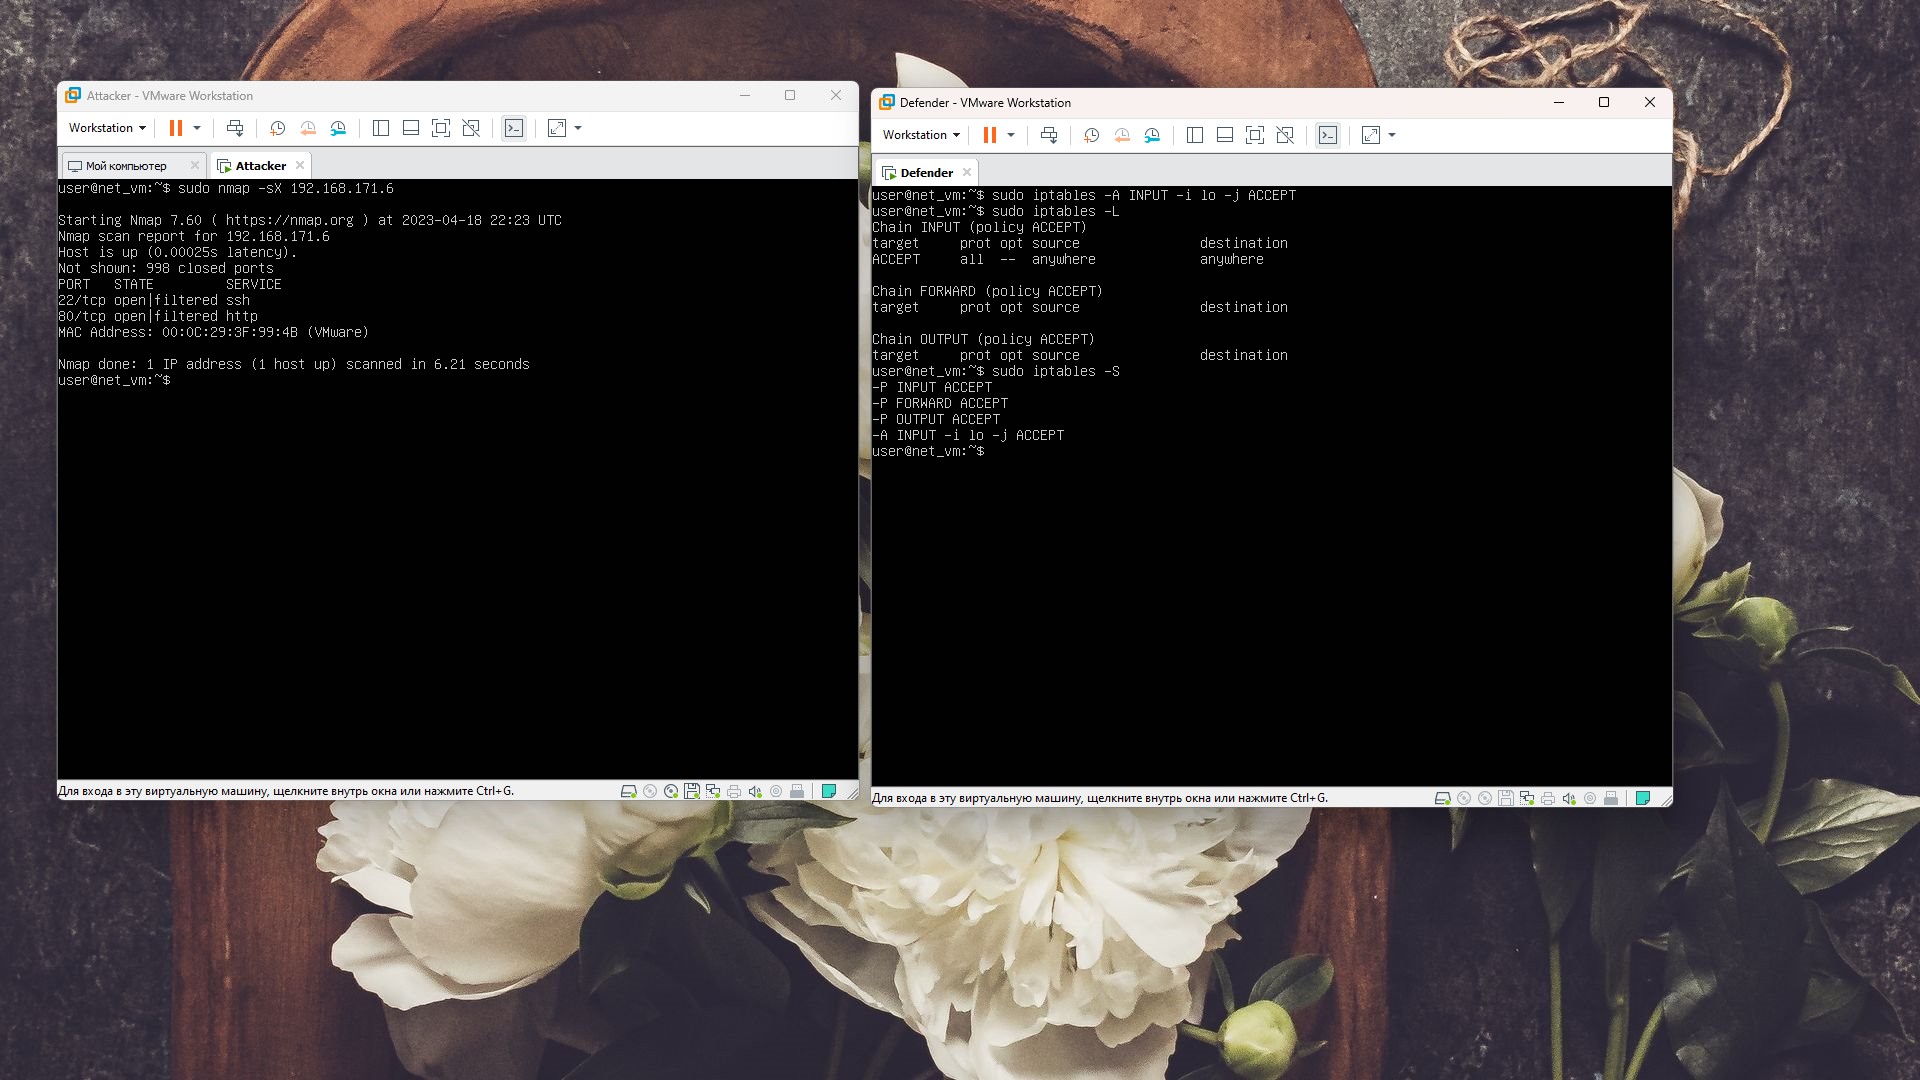
\includegraphics[width=0.85\textwidth]{03_00 (43)}
    \caption{Разрешить все входящие пакеты на интерфейс \textit{lo}}
    \label{img:43}
  \end{figure}

  Сразу можно посмотреть изменения в правилах, при помощи тех же флагов \textit{-L}/\textit{-S}.

  Разрешим все входящие \textit{tcp} соединения на порты 22 и 80 (ssh и http):
  \begin{minted}{bash}
    # Разрешение входящих tcp соединений на 22 порт
    sudo iptables -A INPUT -p tcp -m tcp \\
        --dport 22 -j ACCEPT
    # Разрешение входящих tcp соединений на 80 порт
    sudo iptables -A INPUT -p tcp -m tcp \\
        --dport 80 -j ACCEPT
  \end{minted}

  Однако в ходе данной работы \textit{ssh} использоваться не будет, поэтому 
  удалим правило, разрешающее tcp соединения на 22 порту:

  \begin{figure}[H]
    \centering
    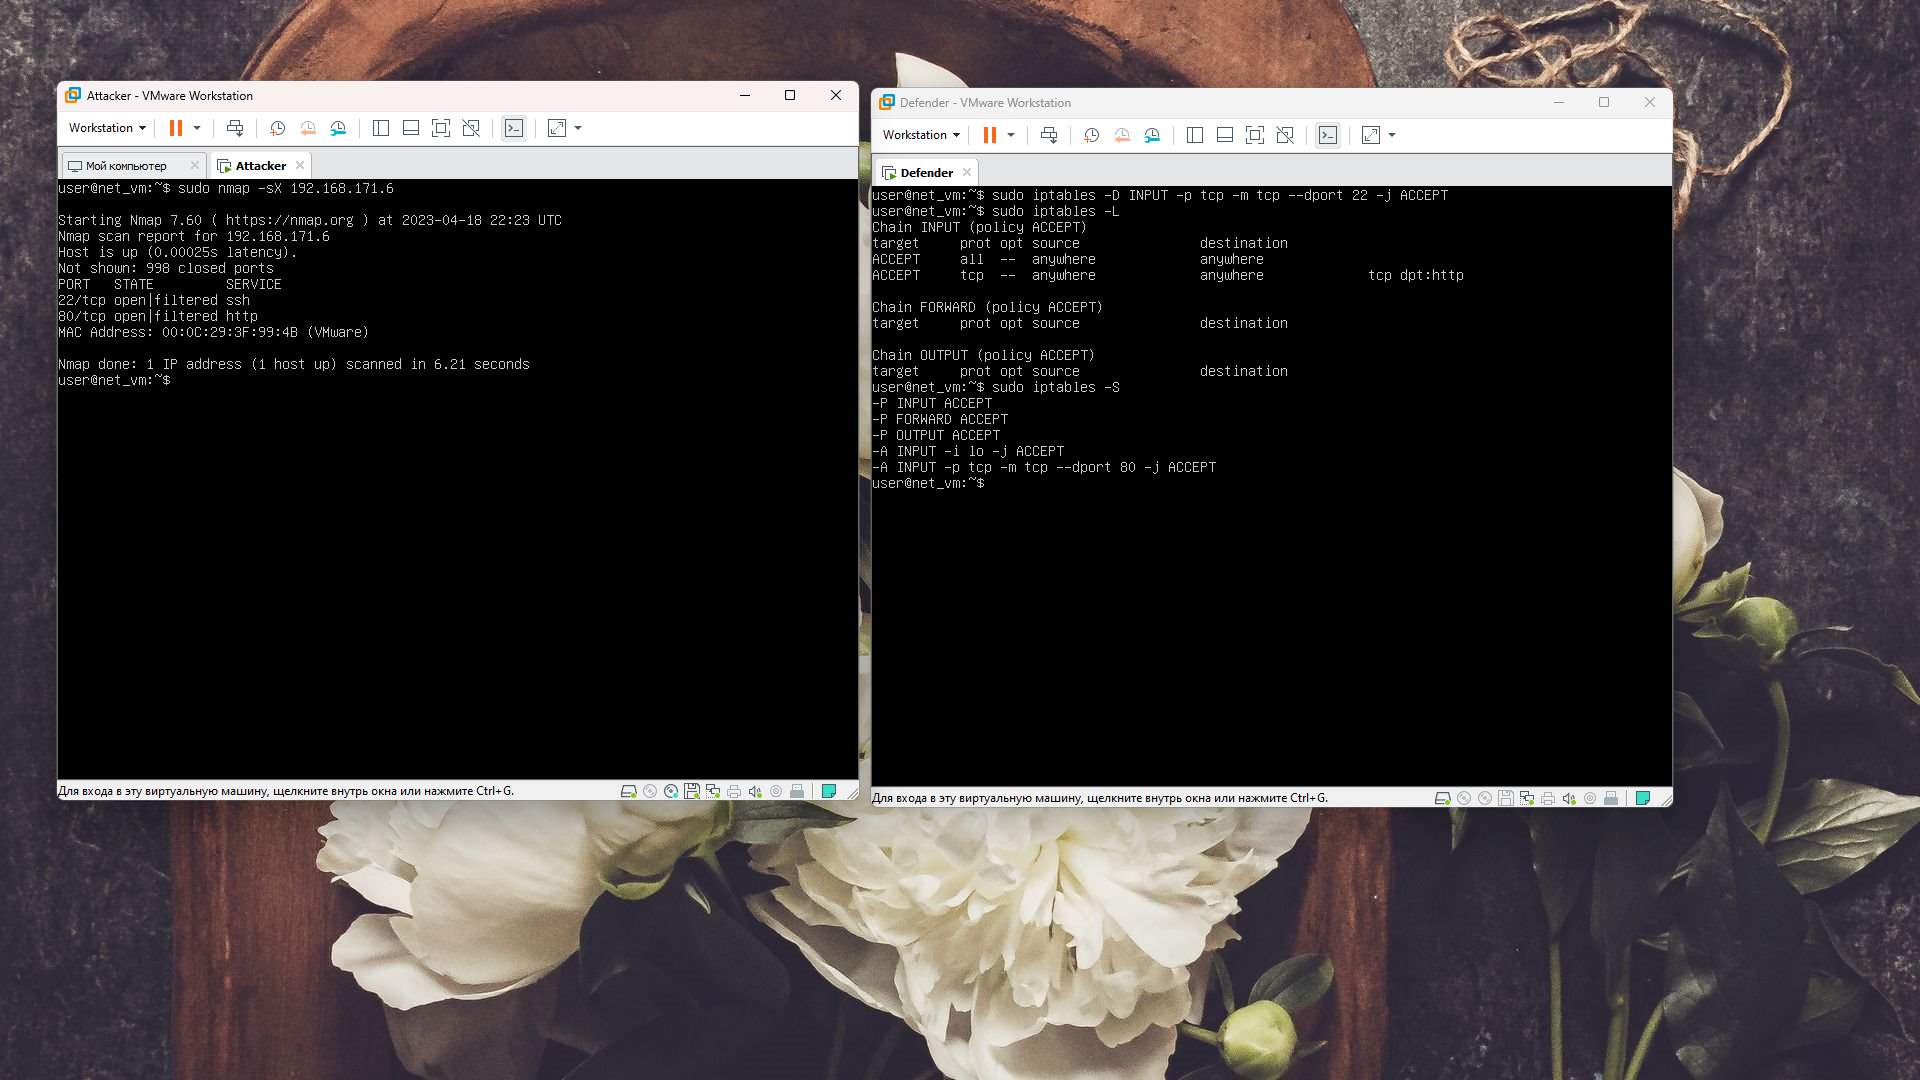
\includegraphics[width=0.85\textwidth]{03_00 (44)}
    \caption{Удаление правила для ssh}
    \label{img:44}
  \end{figure}


  Теперь разрешим все уже установленные сессии (и связанные с ними), чтобы
  можно было пользоваться утилитой \textit{ping} и обновлять пакеты:
  
  \begin{figure}[H]
    \centering
    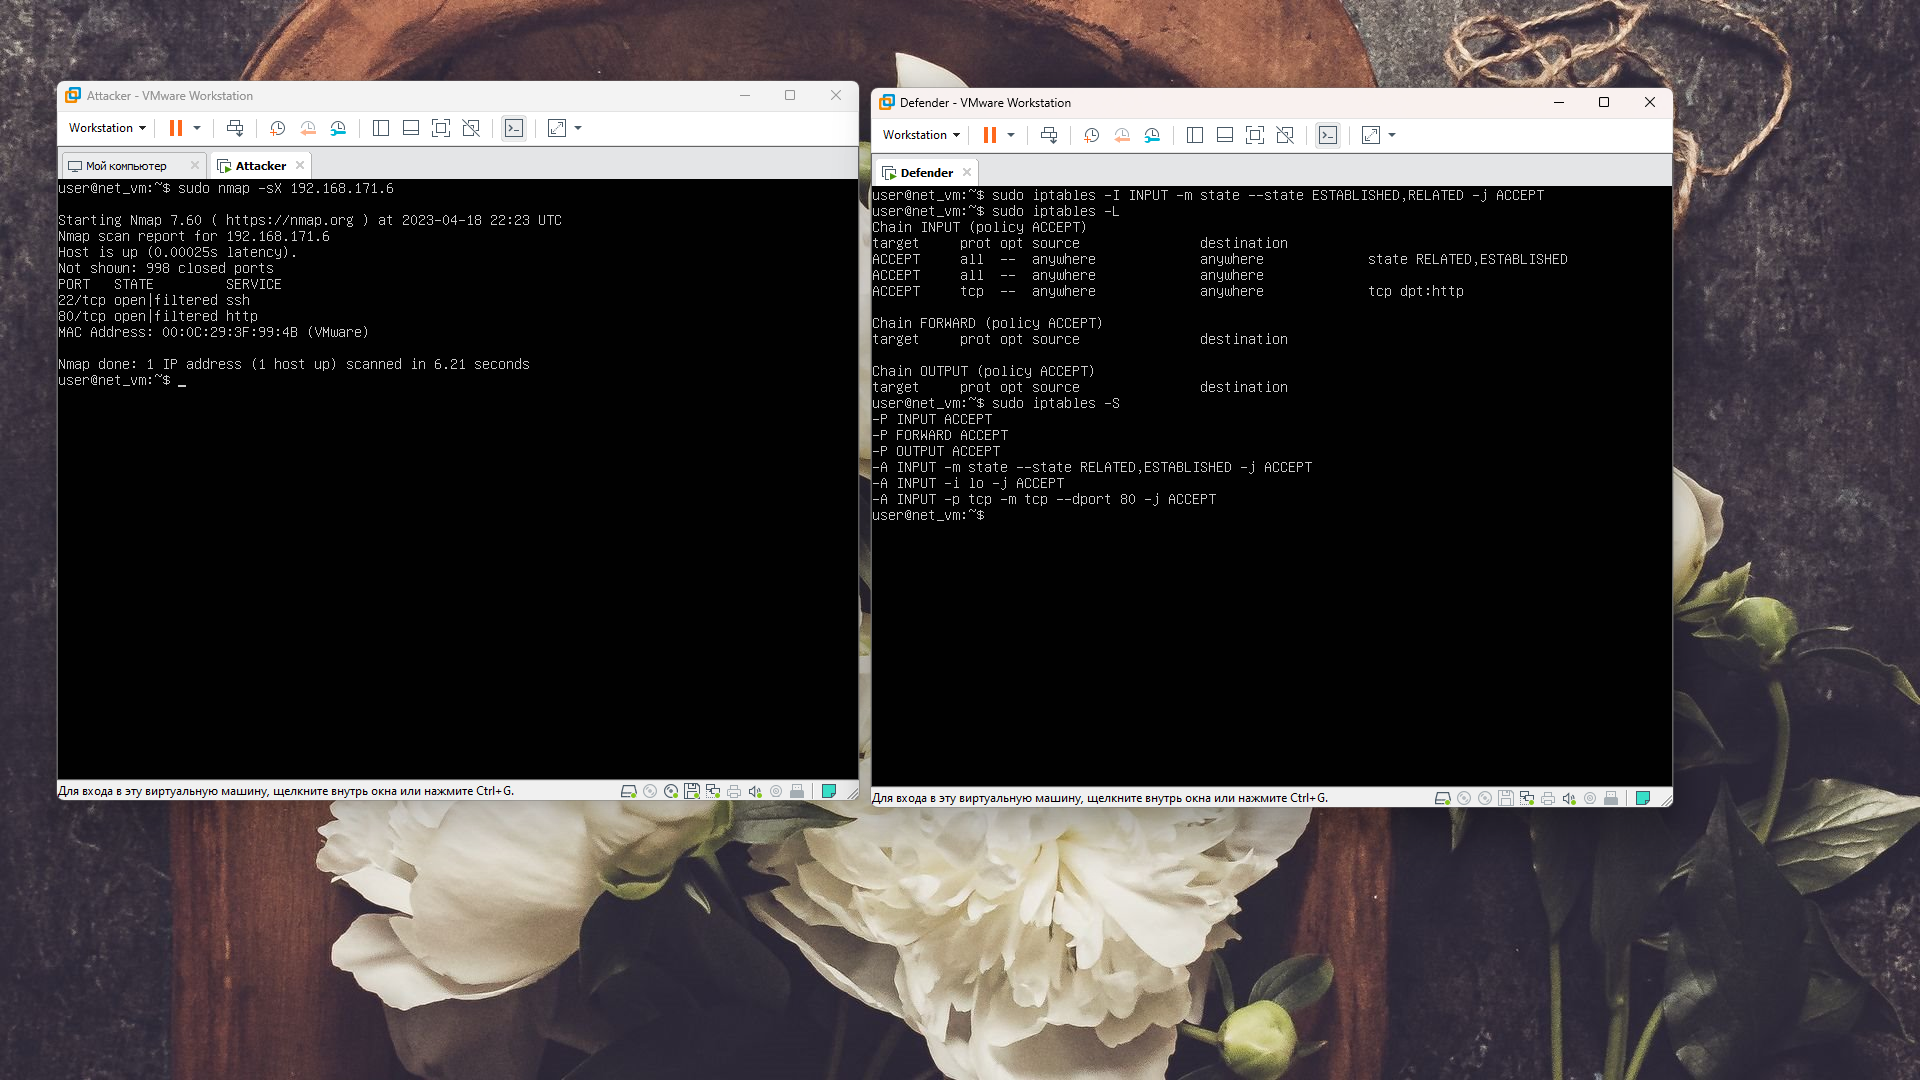
\includegraphics[width=0.85\textwidth]{03_00 (45)}
    \caption{\textit{iptables -I INPUT -m state --state ESTABLISHED,RELATED -j ACCEPT}}
    \label{img:45}
  \end{figure}

  Все основные разрешающие правила созданы и настроены, теперь запретим все остальные входящие 
  соединения и разрешим все исходящие:

  \begin{figure}[H]
    \centering
    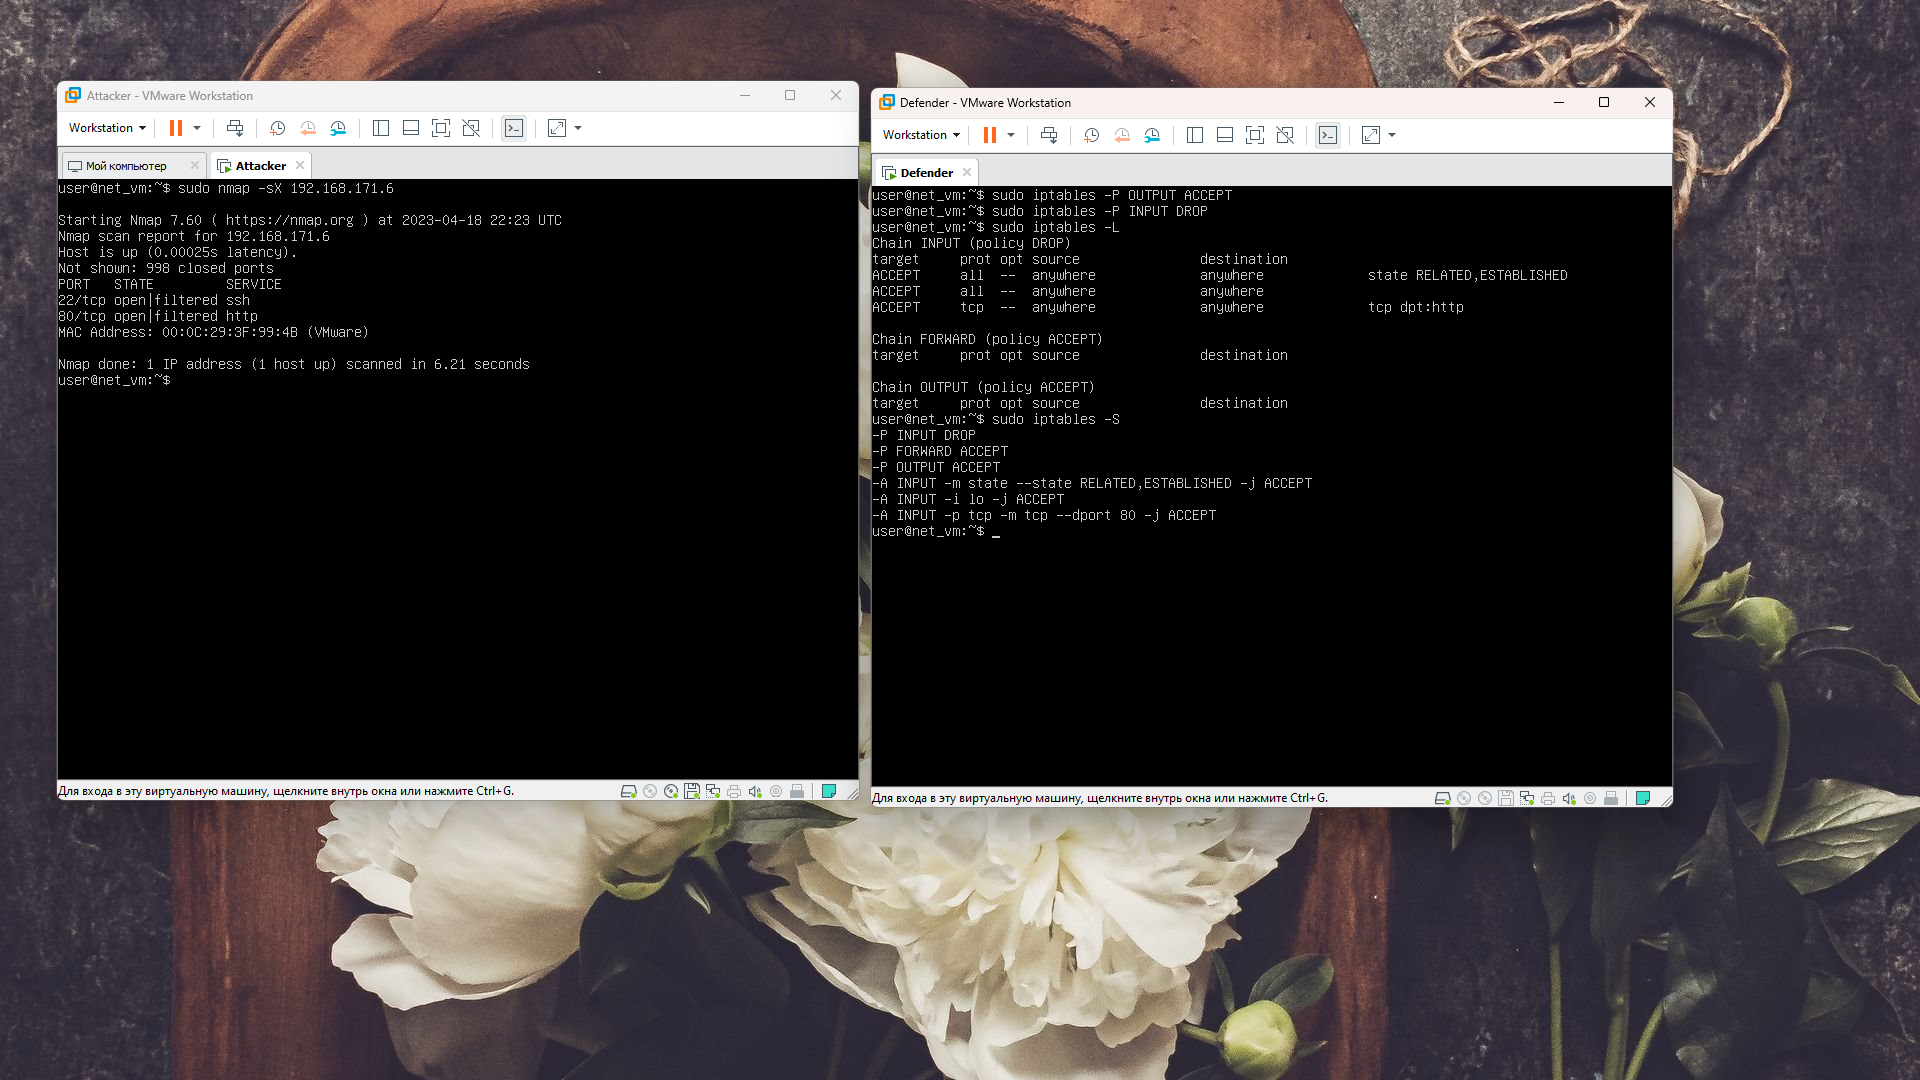
\includegraphics[width=0.85\textwidth]{03_00 (46)}
    \caption{Запретить все входящие, кроме ранее разрешенных, и разрешить все исходящие}
    \label{img:46}
  \end{figure}

  Также было бы отлично защититься от \textit{NULL} и \textit{SYN} сканирований,
  для этого запретим все вхоядщие нулевые и \textit{syn} пакеты:

  \begin{figure}[H]
    \centering
    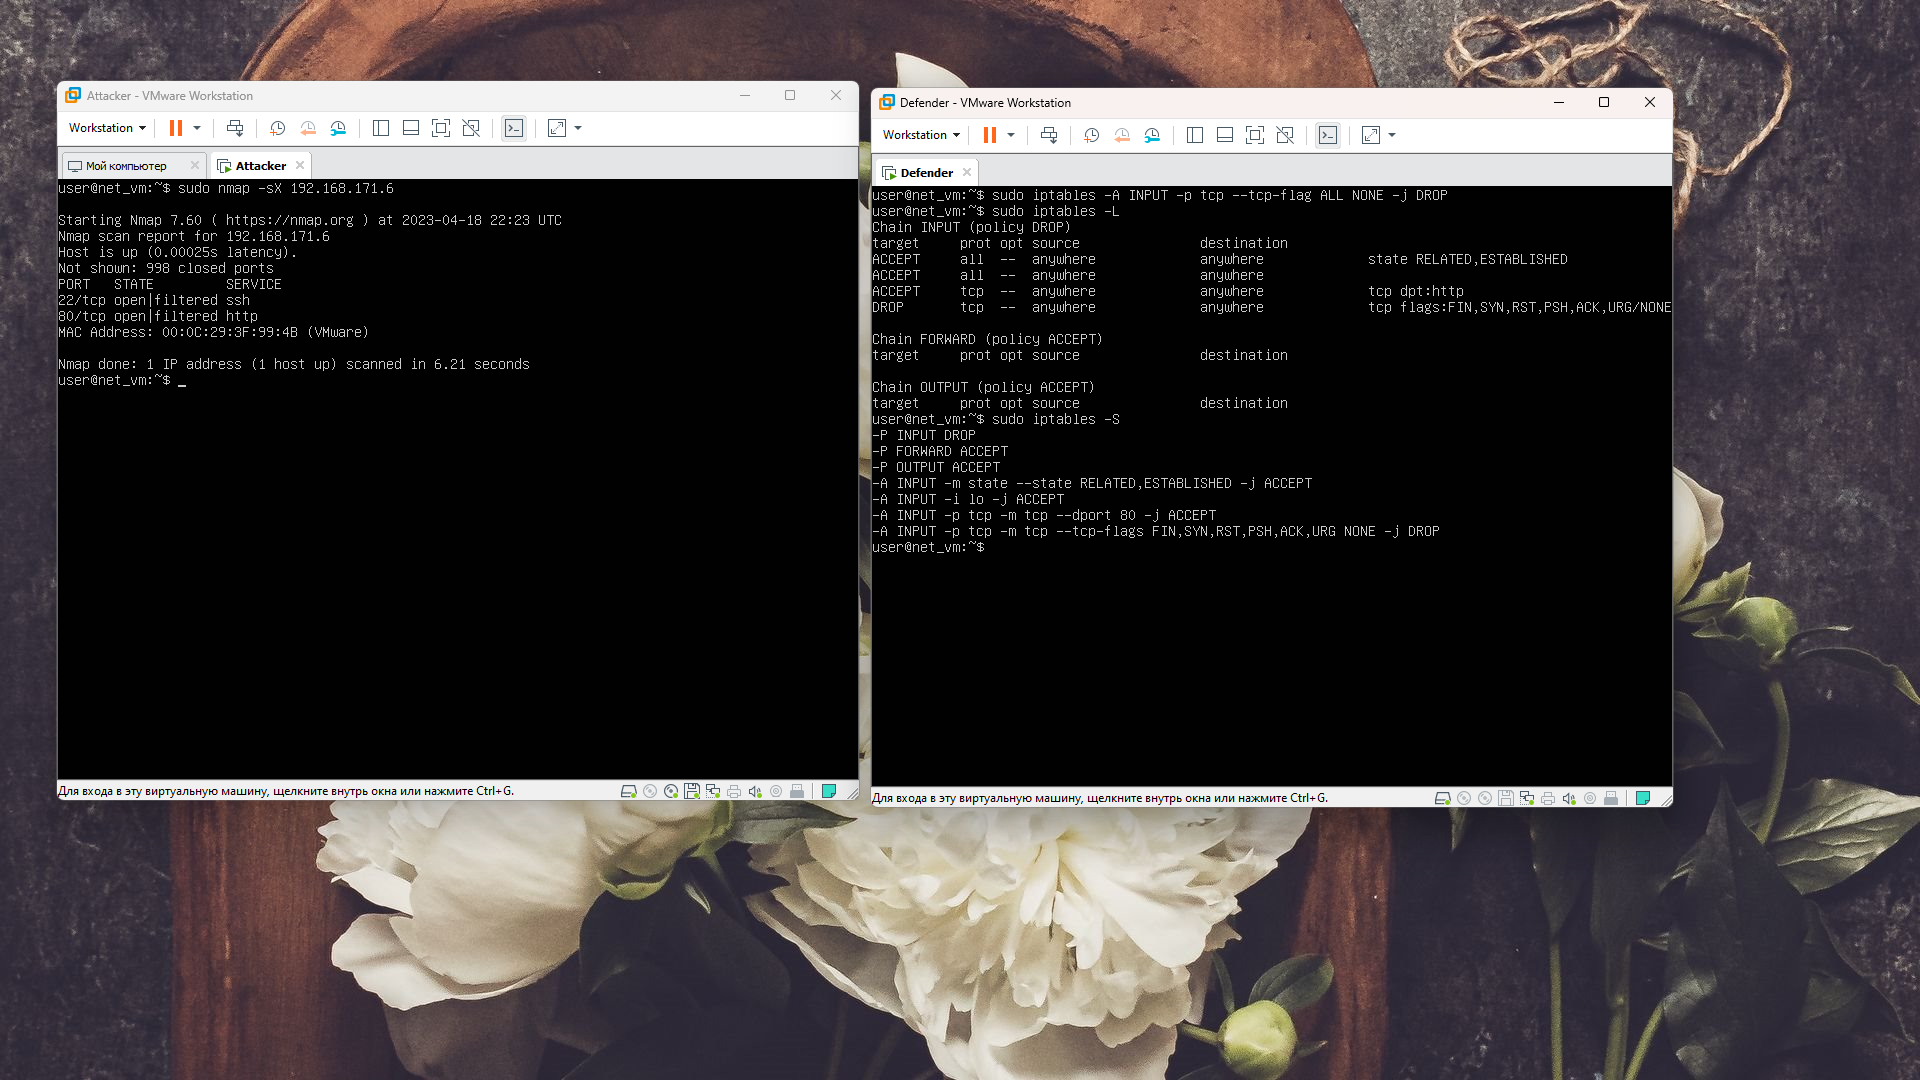
\includegraphics[width=0.85\textwidth]{03_00 (47)}
    \caption{Запрет \textit{NULL} \textit{TCP}-пакетов}
    \label{img:47}
  \end{figure}

  \begin{figure}[H]
    \centering
    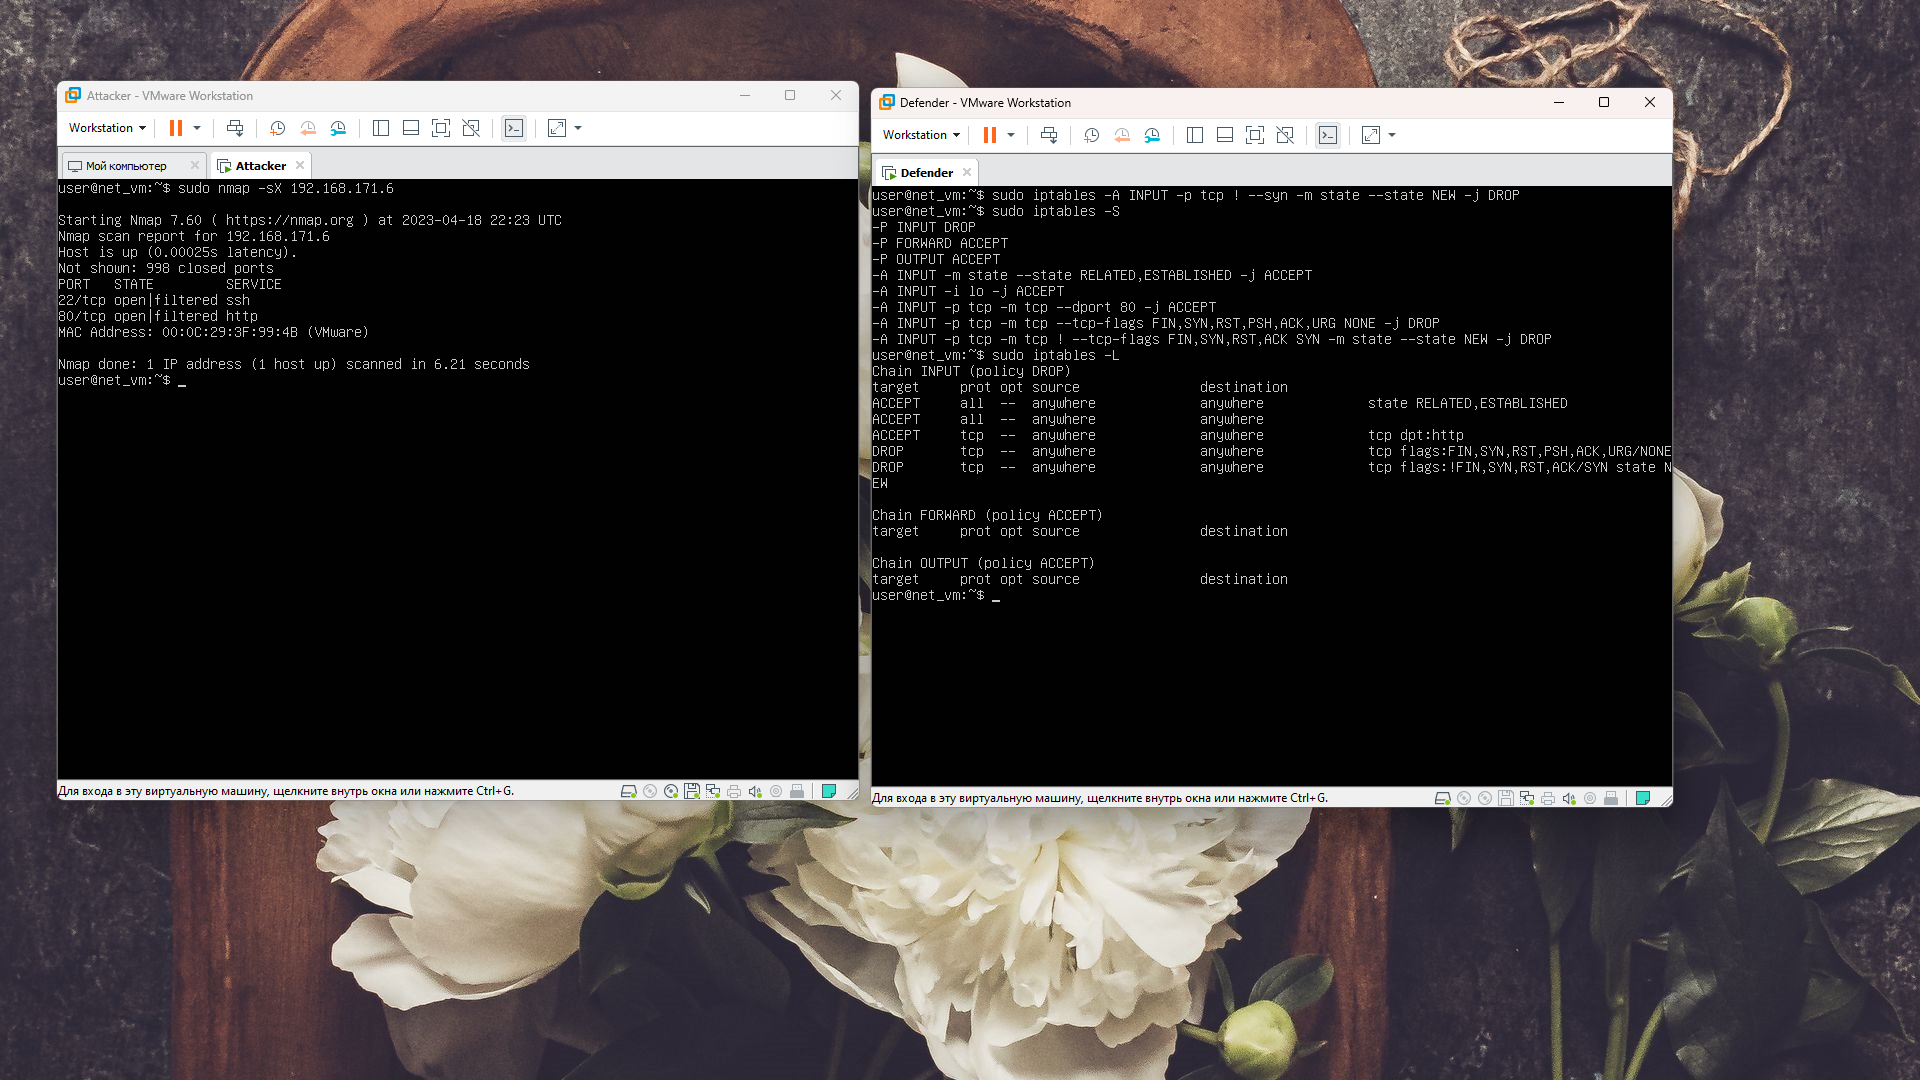
\includegraphics[width=0.85\textwidth]{03_00 (48)}
    \caption{Запрет не \textit{NEW} \textit{SYN} пакетов}
    \label{img:48}
  \end{figure}

  Также запретим все входящие пакеты, используемые при \textit{XMas} сканировании,
  что еще сильнее обезопасит систему:

  \begin{figure}[H]
    \centering
    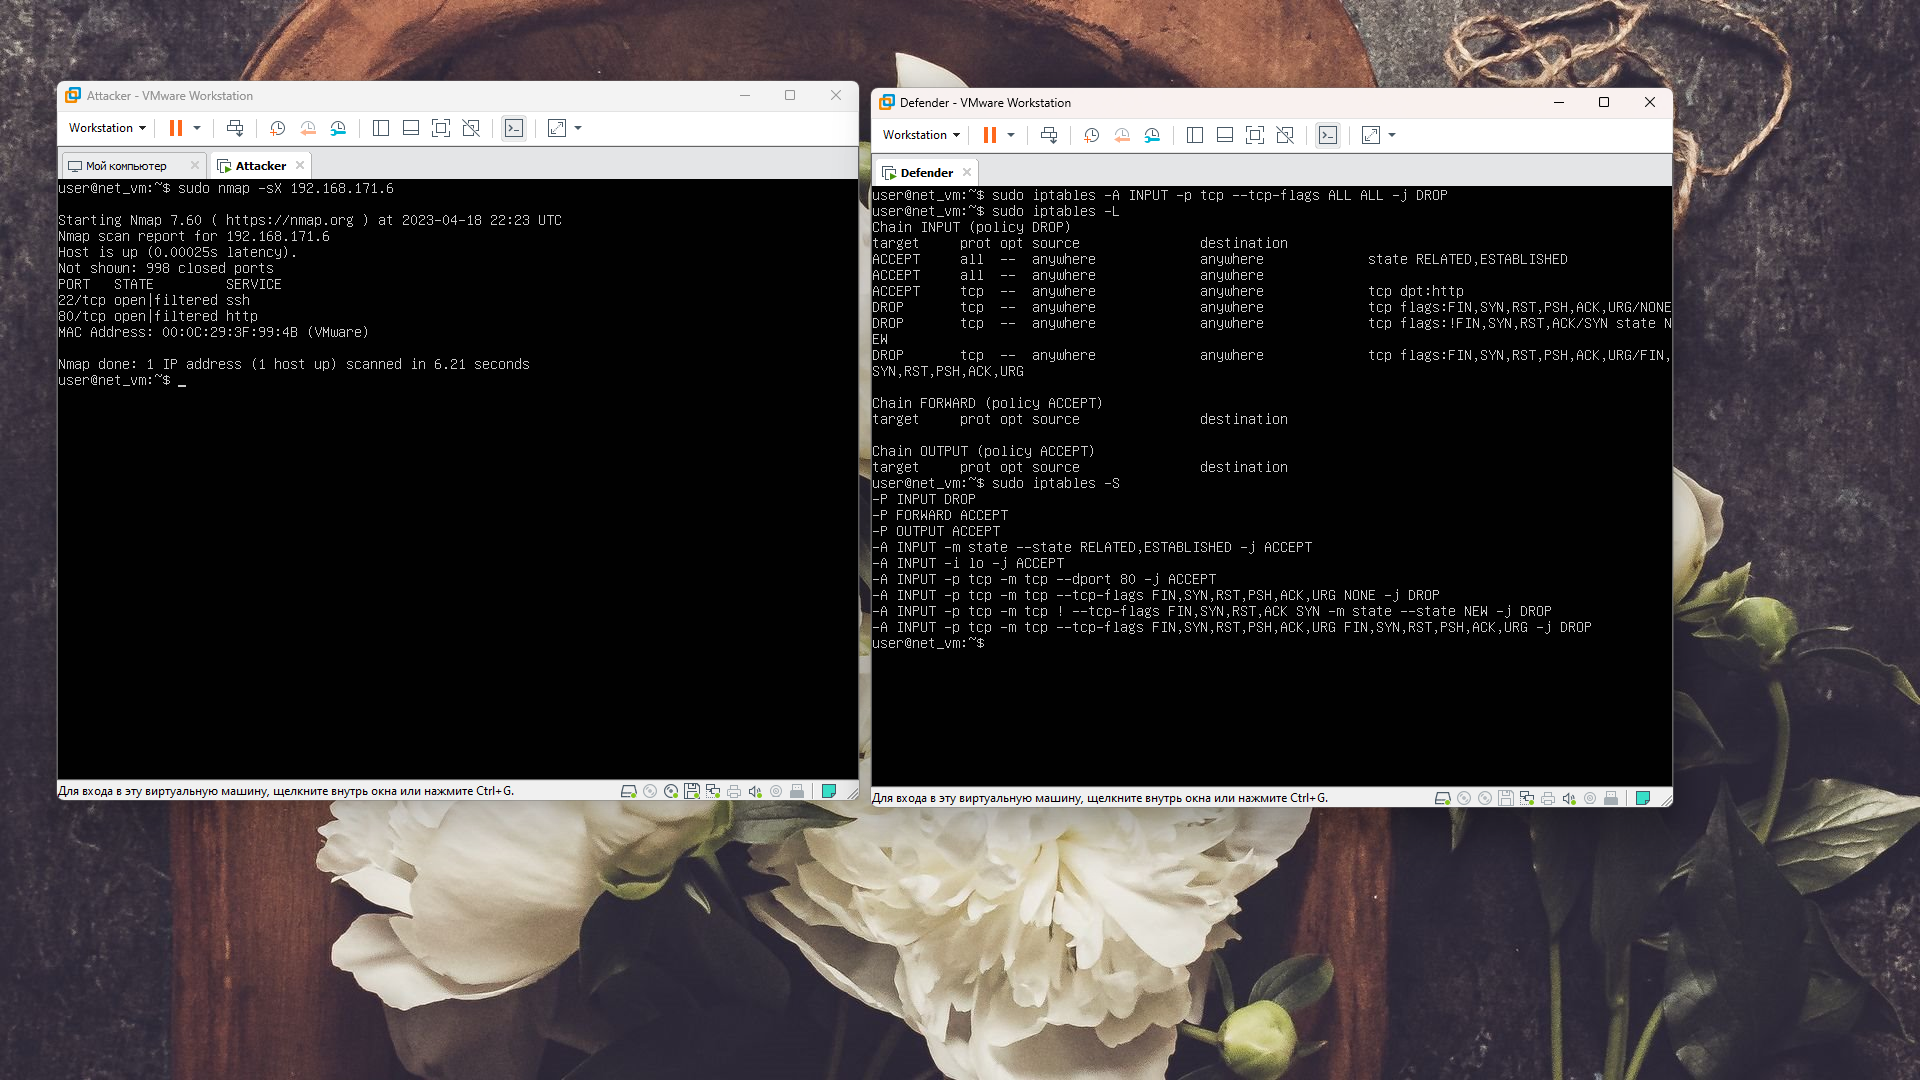
\includegraphics[width=0.85\textwidth]{03_00 (49)}
    \caption{Защита от \textit{XMas} сканирования}
    \label{img:49}
  \end{figure}

  Правила созданы, но еще не действуют, чтобы их активировать установим специальный пакет:

  \begin{figure}[H]
    \centering
    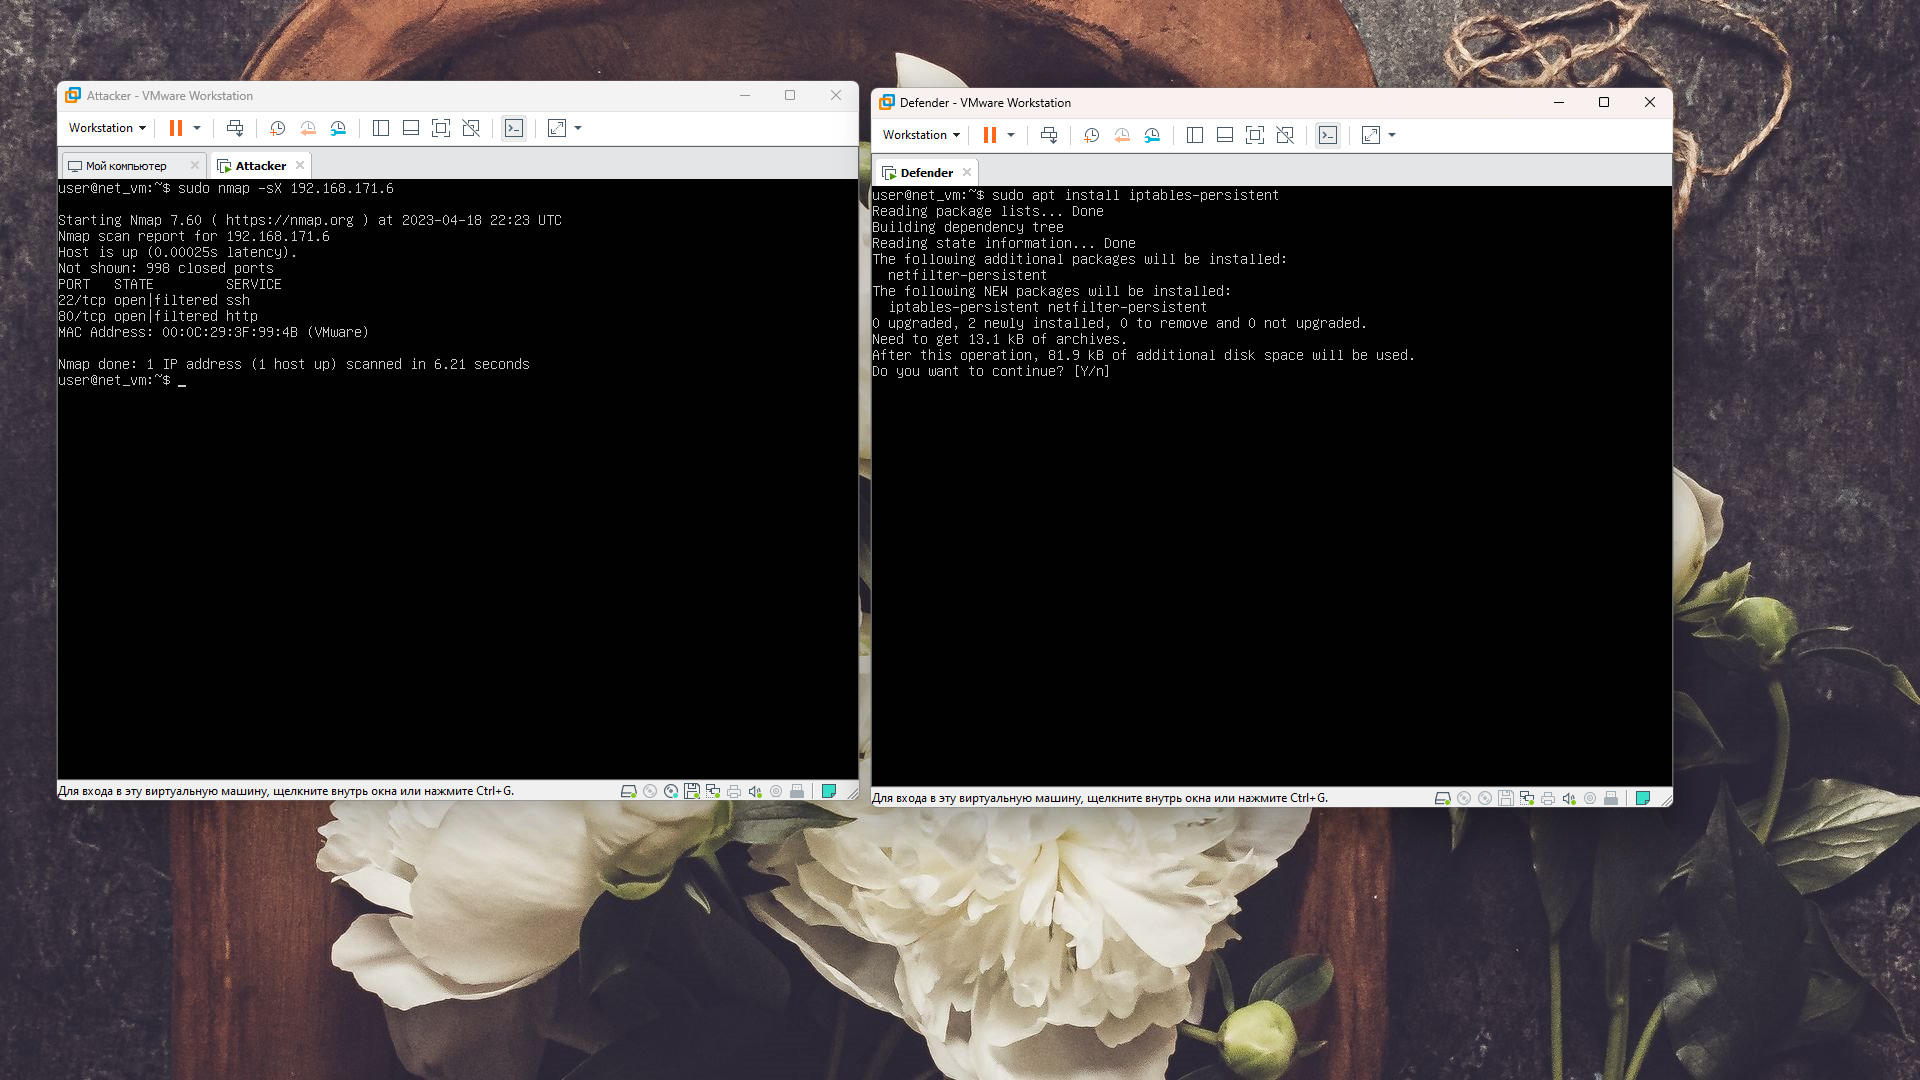
\includegraphics[width=0.85\textwidth]{03_00 (50)}
    \caption{\textit{apt install iptables-persistent}}
    \label{img:50}
  \end{figure}

  \begin{figure}[H]
    \centering
    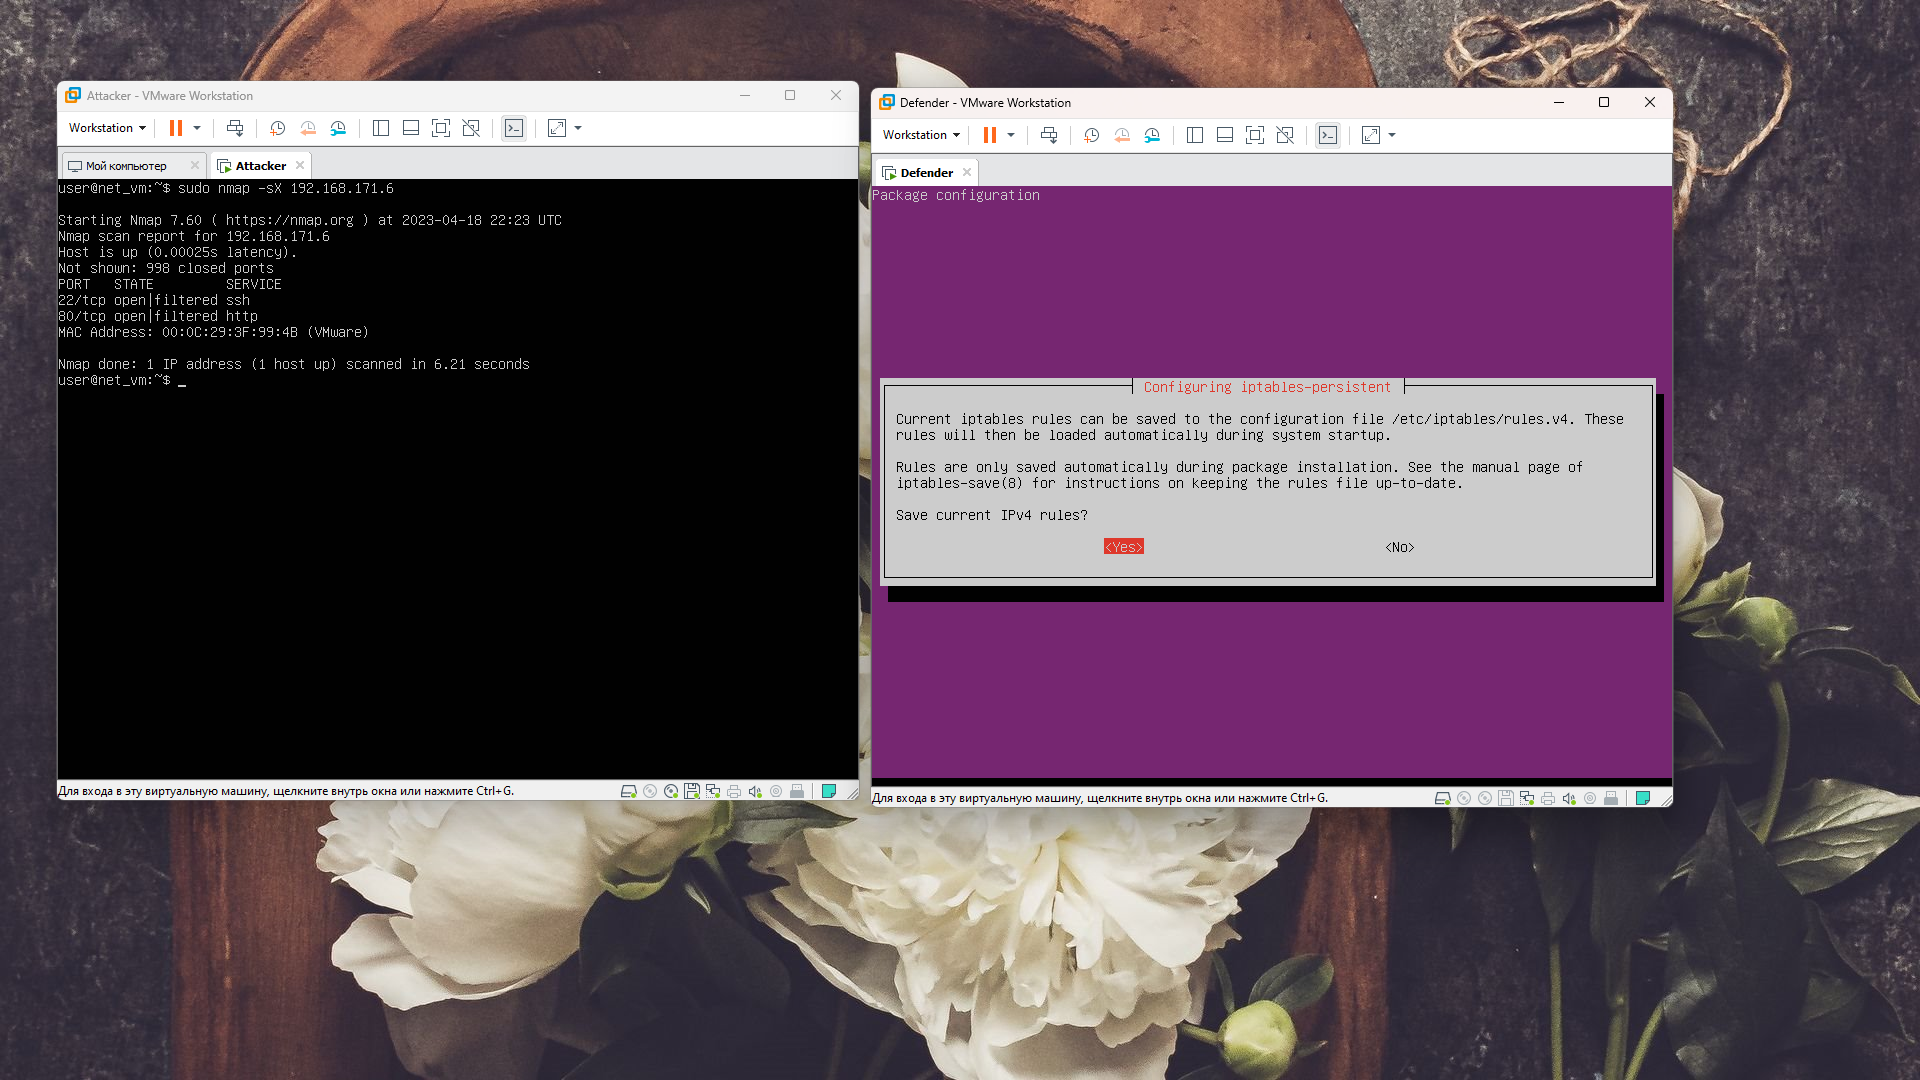
\includegraphics[width=0.85\textwidth]{03_00 (51)}
    \caption{Yes - автоматически применять все правила (без перезагрузки системы)}
    \label{img:51}
  \end{figure}

  Теперь, когда все правила настроены, попробуем снова выполнить \textit{XMas} сканирование
  и посмотрим, что изменилось:

  \begin{figure}[H]
    \centering
    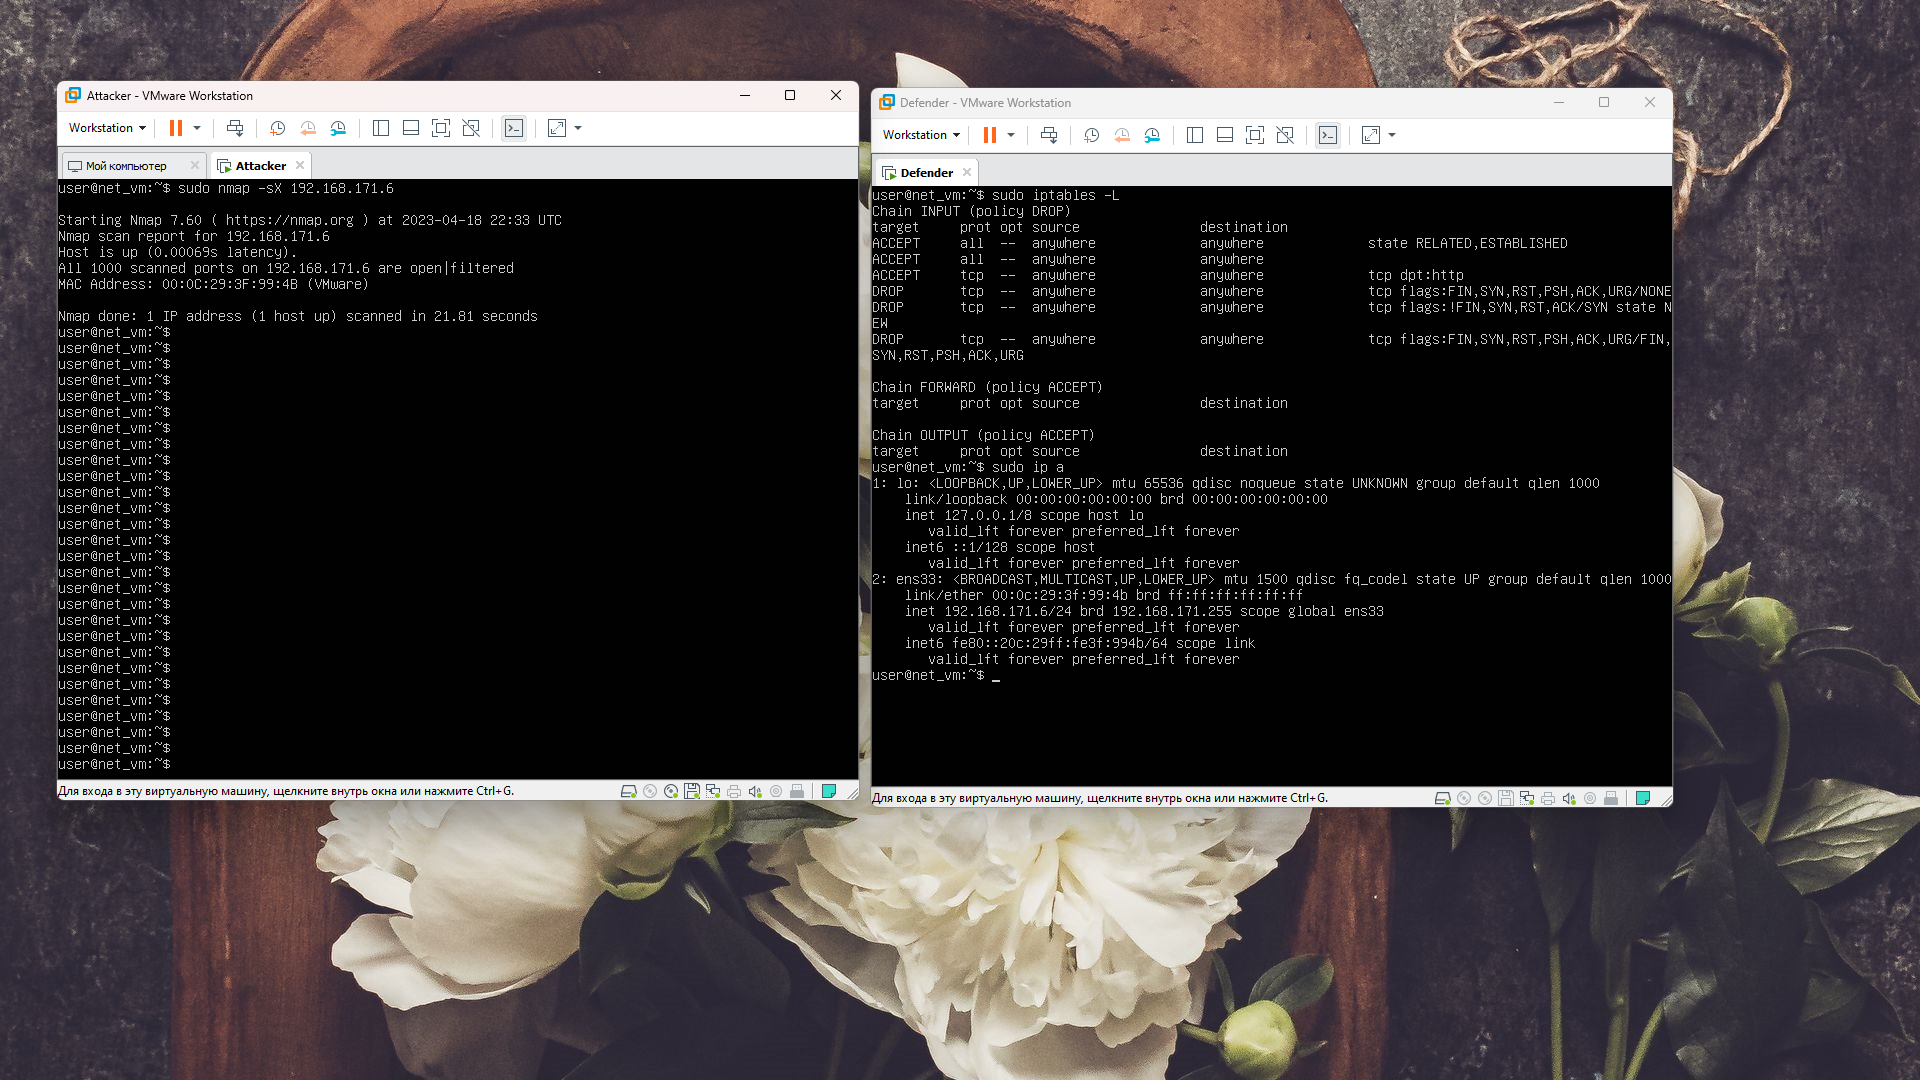
\includegraphics[width=0.85\textwidth]{03_00 (53)}
    \caption{\textit{XMas} сканирование атакуемой машины}
    \label{img:52}
  \end{figure}

  Как видно, теперь \textit{nmap} не удалось определит по факту открытые порты, то
  есть настроенные правила отработали корректно.

  \subsection{WAF}

  Теперь загрузим репозиторий с набором более серьезных настроек безопасности для \textit{apache2}:

  \begin{figure}[H]
    \centering
    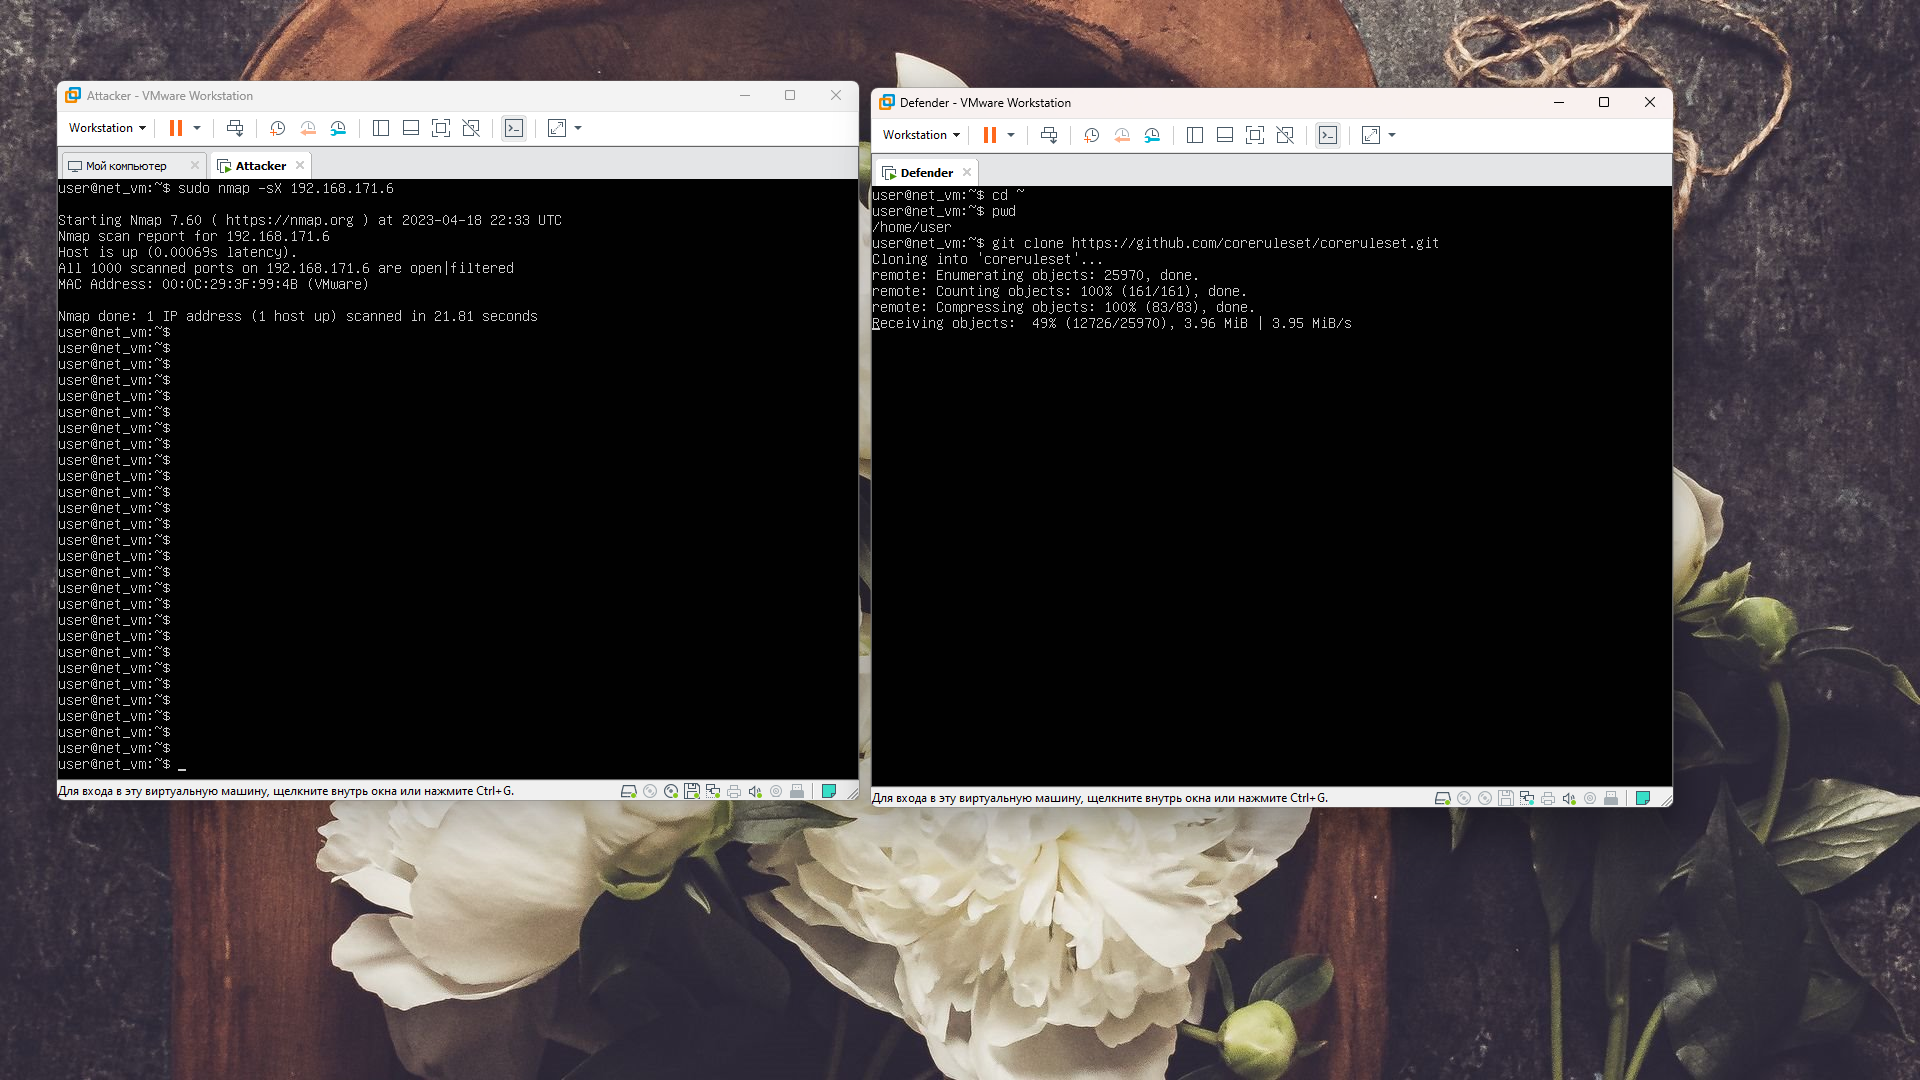
\includegraphics[width=0.85\textwidth]{03_00 (54)}
    \caption{coreruleset - набор настроек безопасности}
    \label{img:54}
  \end{figure}

  Скопируем пример конфигу как основной, а также установим все правила в систему:

  \begin{figure}[H]
    \centering
    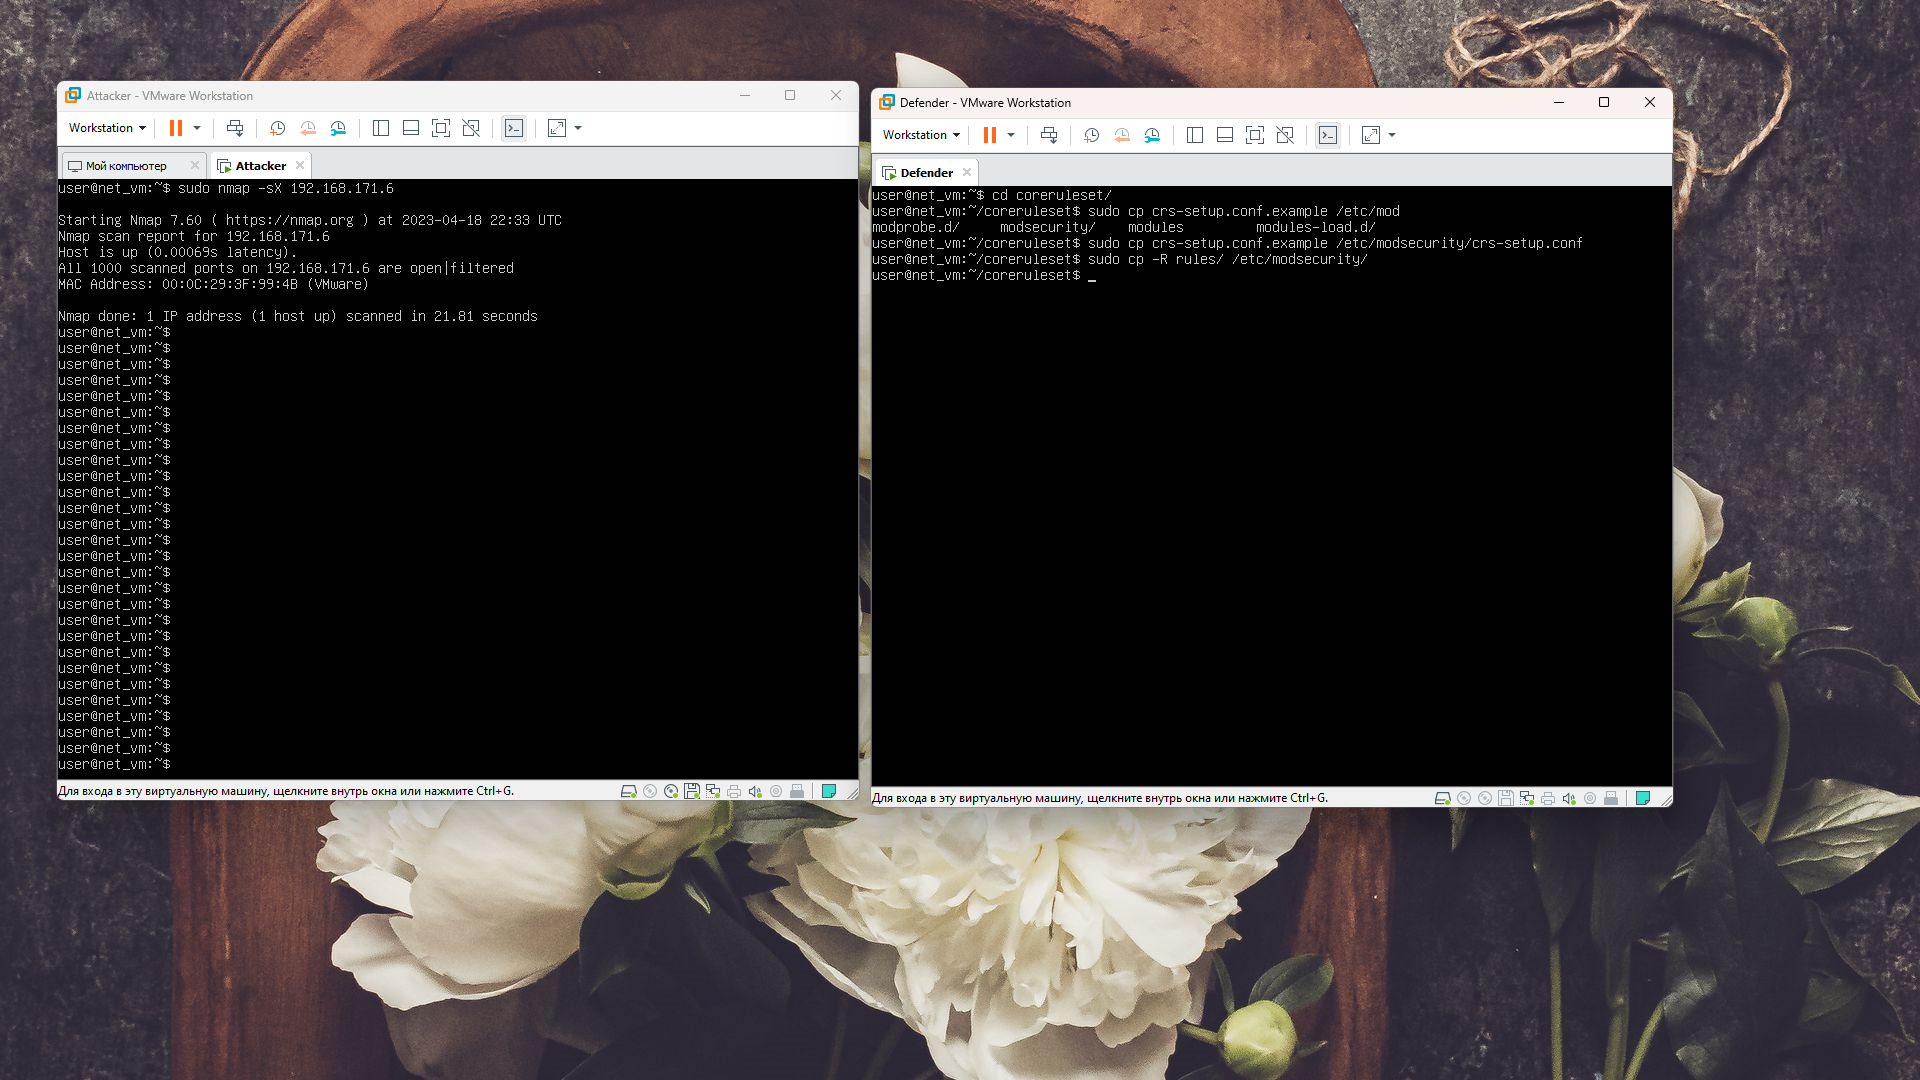
\includegraphics[width=0.85\textwidth]{03_00 (55)}
    \caption{Установка скачанных правил}
    \label{img:55}
  \end{figure}

  Модуль безопасности требует дополнительной настройки - возьмем за основу
  пример конфига, скопируем его по нужному пути:

  \begin{figure}[H]
    \centering
    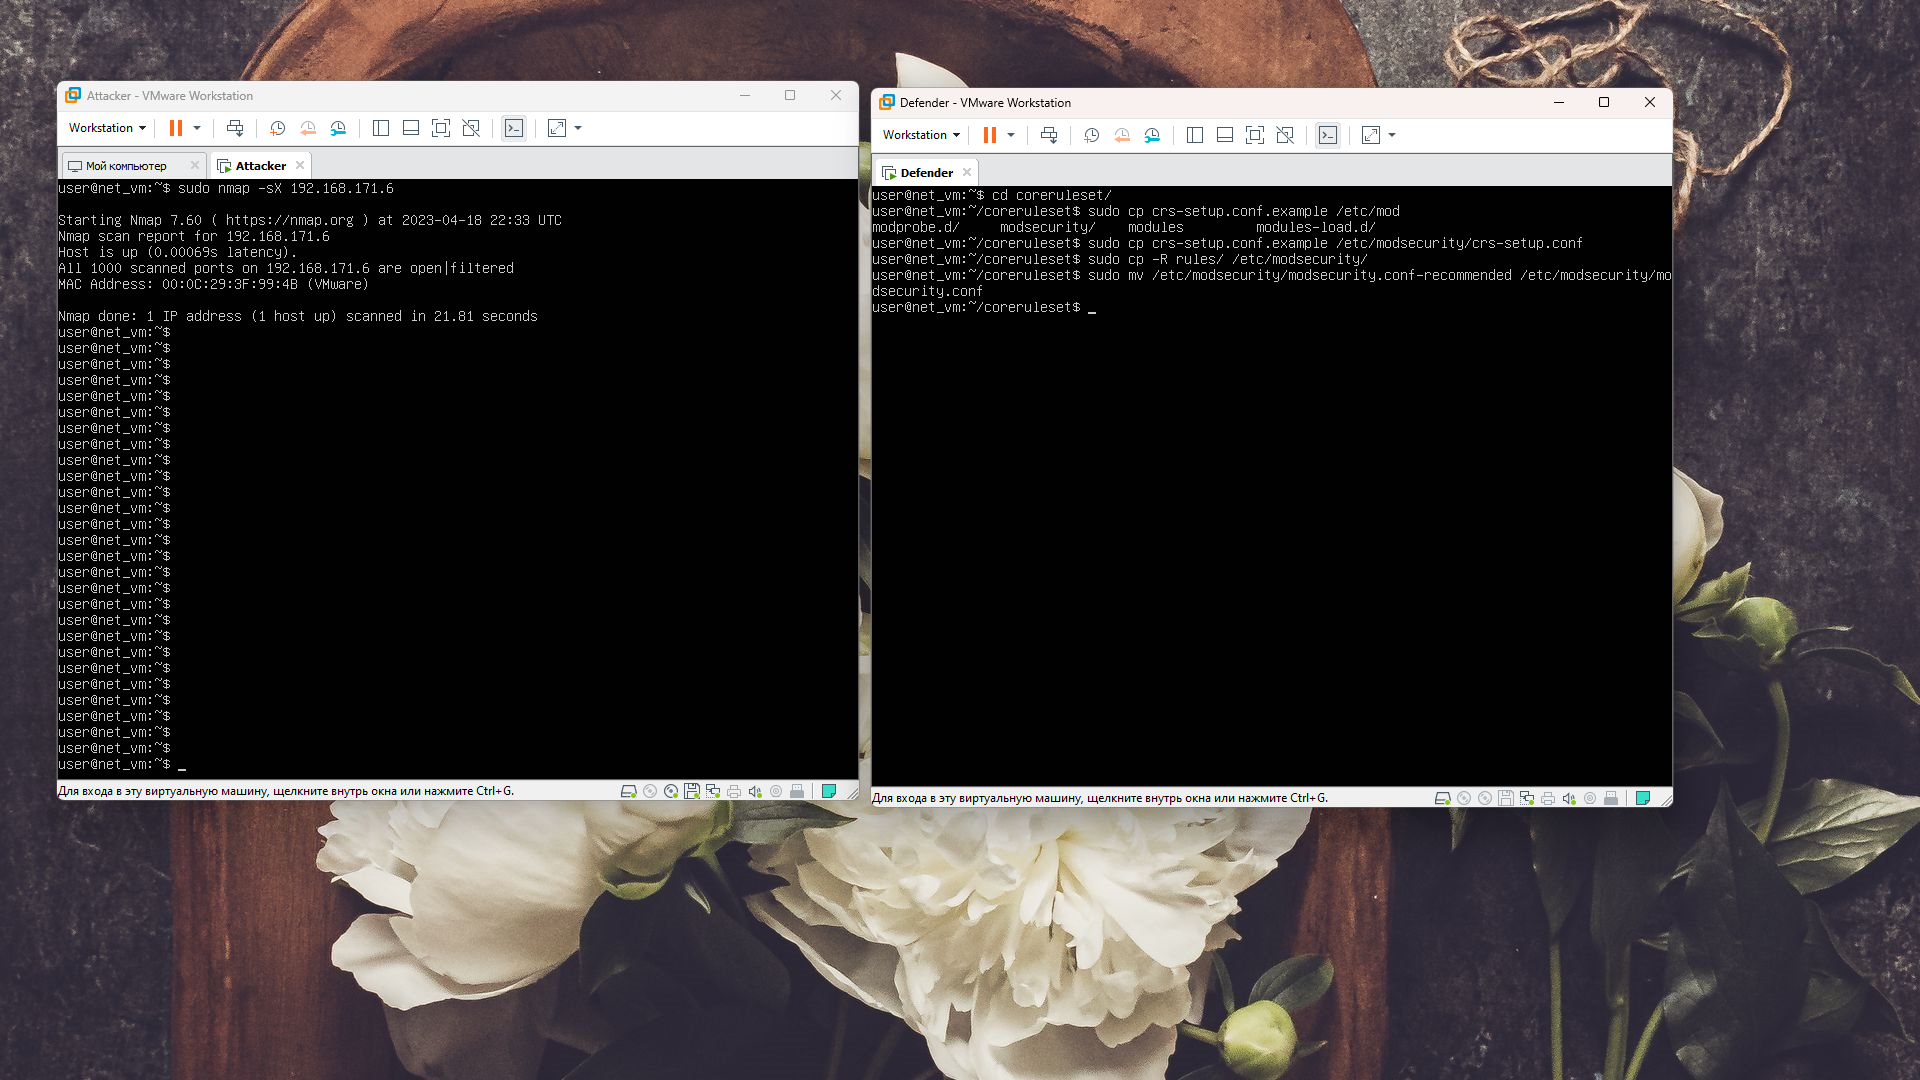
\includegraphics[width=0.85\textwidth]{03_00 (56)}
    \caption{Установка примера конфигурации как основной конфигурации}
    \label{img:56}
  \end{figure}

  А затем откроем для редактирования и внесем изменения - включим \textit{SecRuleEngine}:

  \begin{figure}[H]
    \centering
    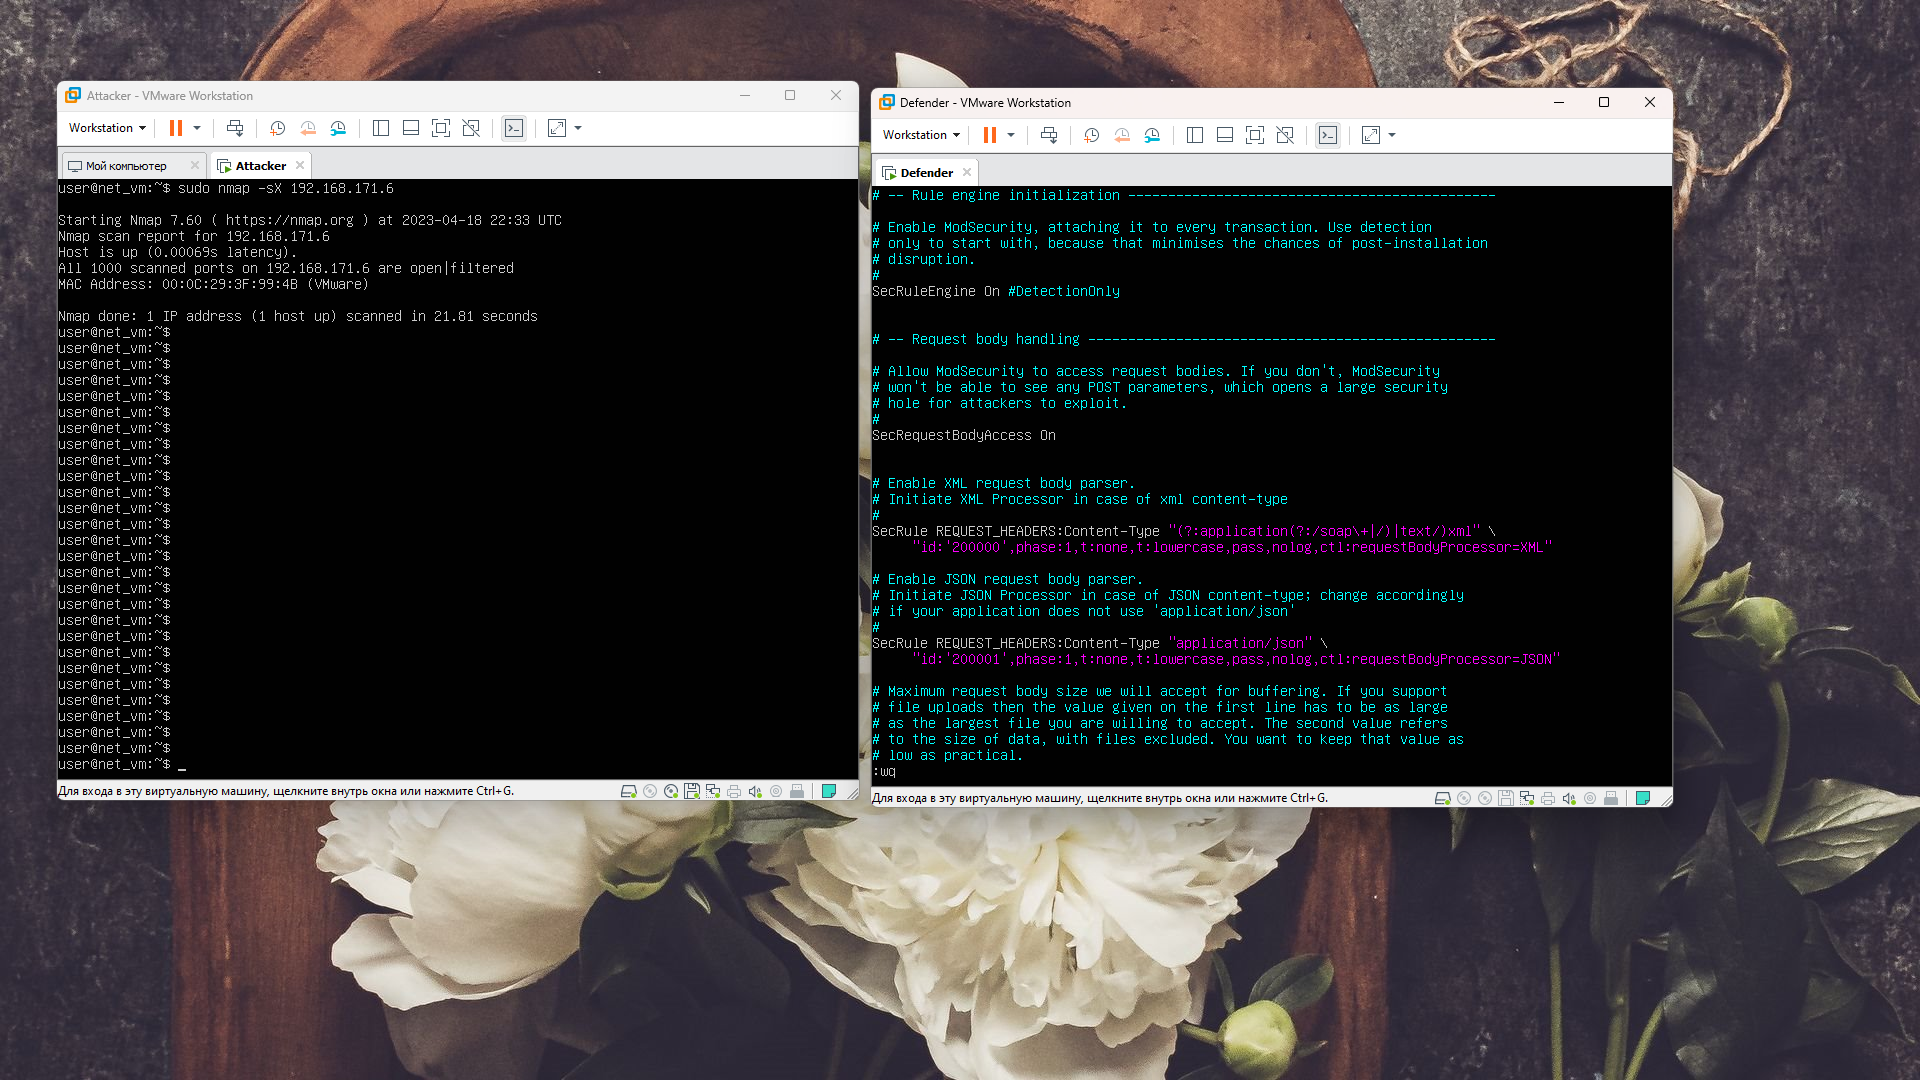
\includegraphics[width=0.85\textwidth]{03_00 (58)}
    \caption{Измененный конфиге - включен модуль безопасности (DetectionOnly -> On)}
    \label{img:58}
  \end{figure}

  Теперь подключим установленные и настроенные правила к \textit{web} серверу \textit{apache}:

  \begin{figure}[H]
    \centering
    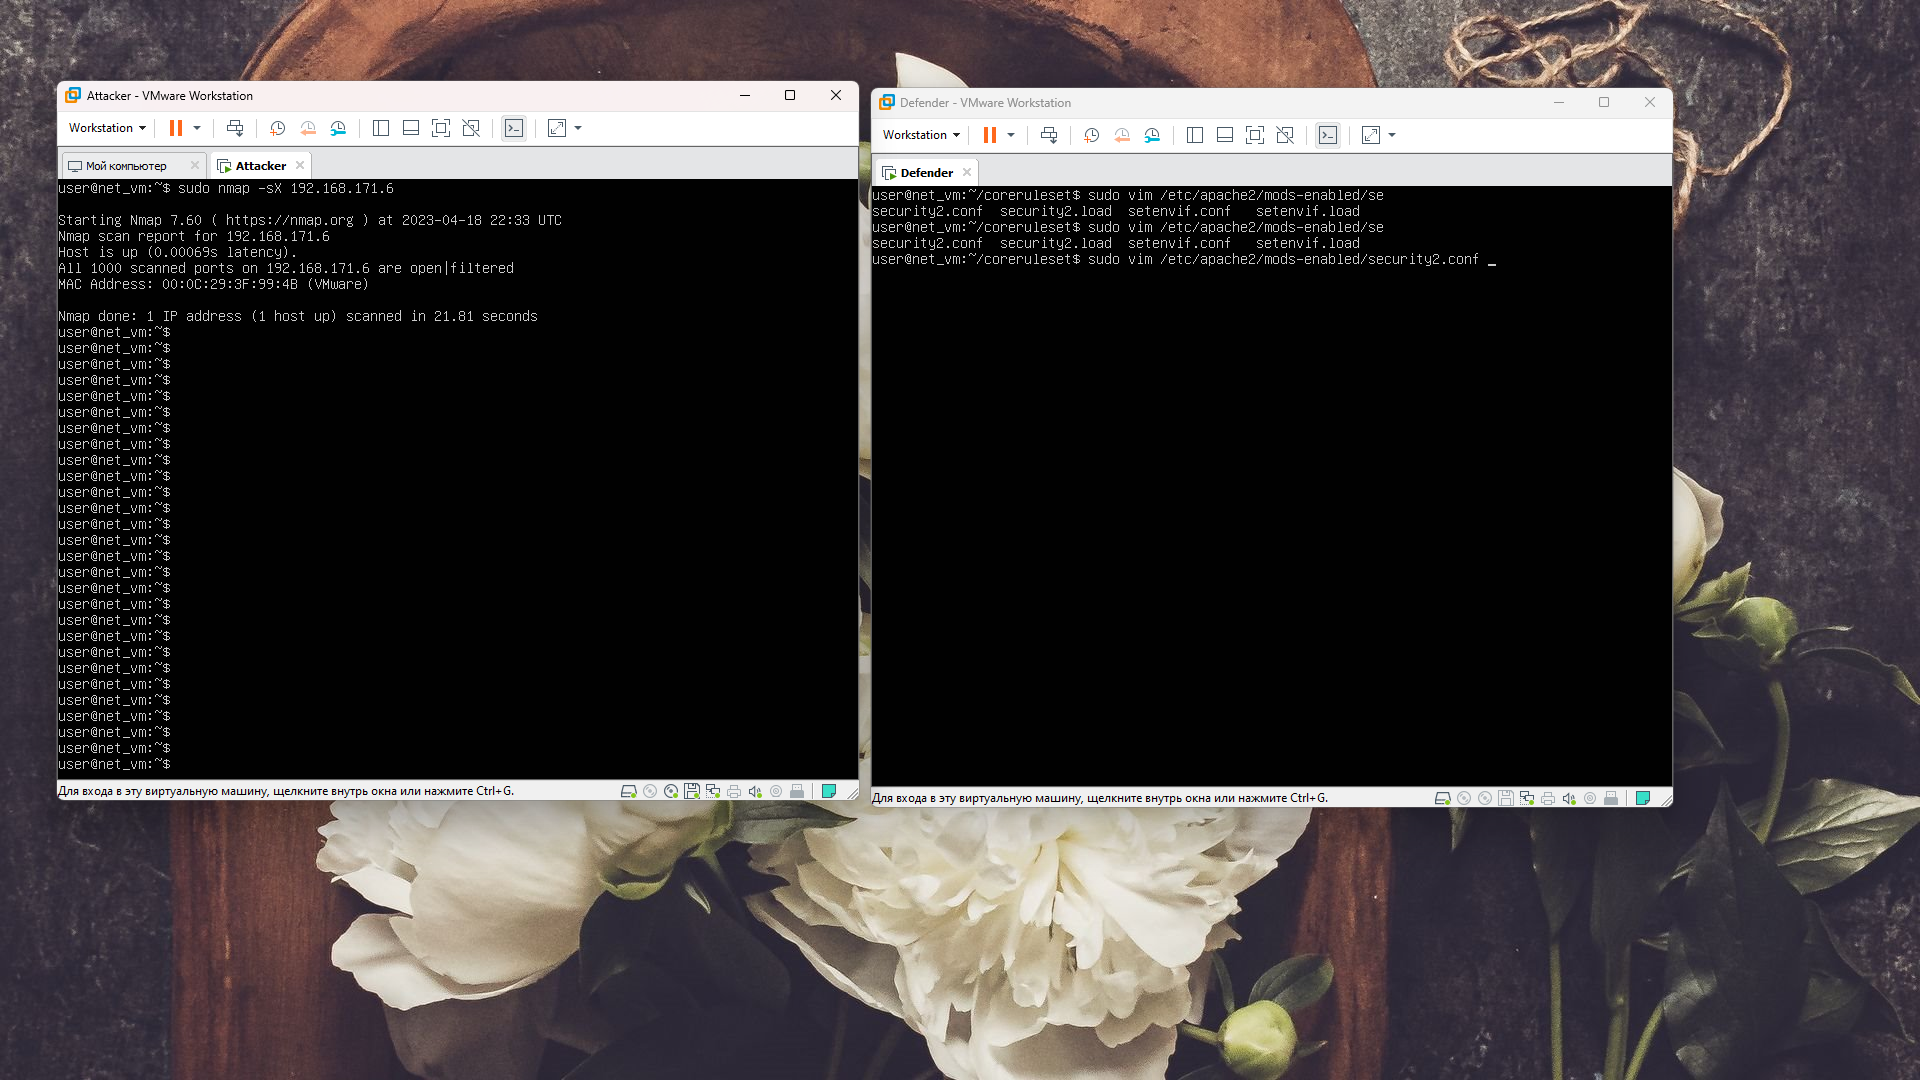
\includegraphics[width=0.85\textwidth]{03_00 (59)}
    \caption{Открываем конфиг \textit{apache}}
    \label{img:59}
  \end{figure}

  \begin{figure}[H]
    \centering
    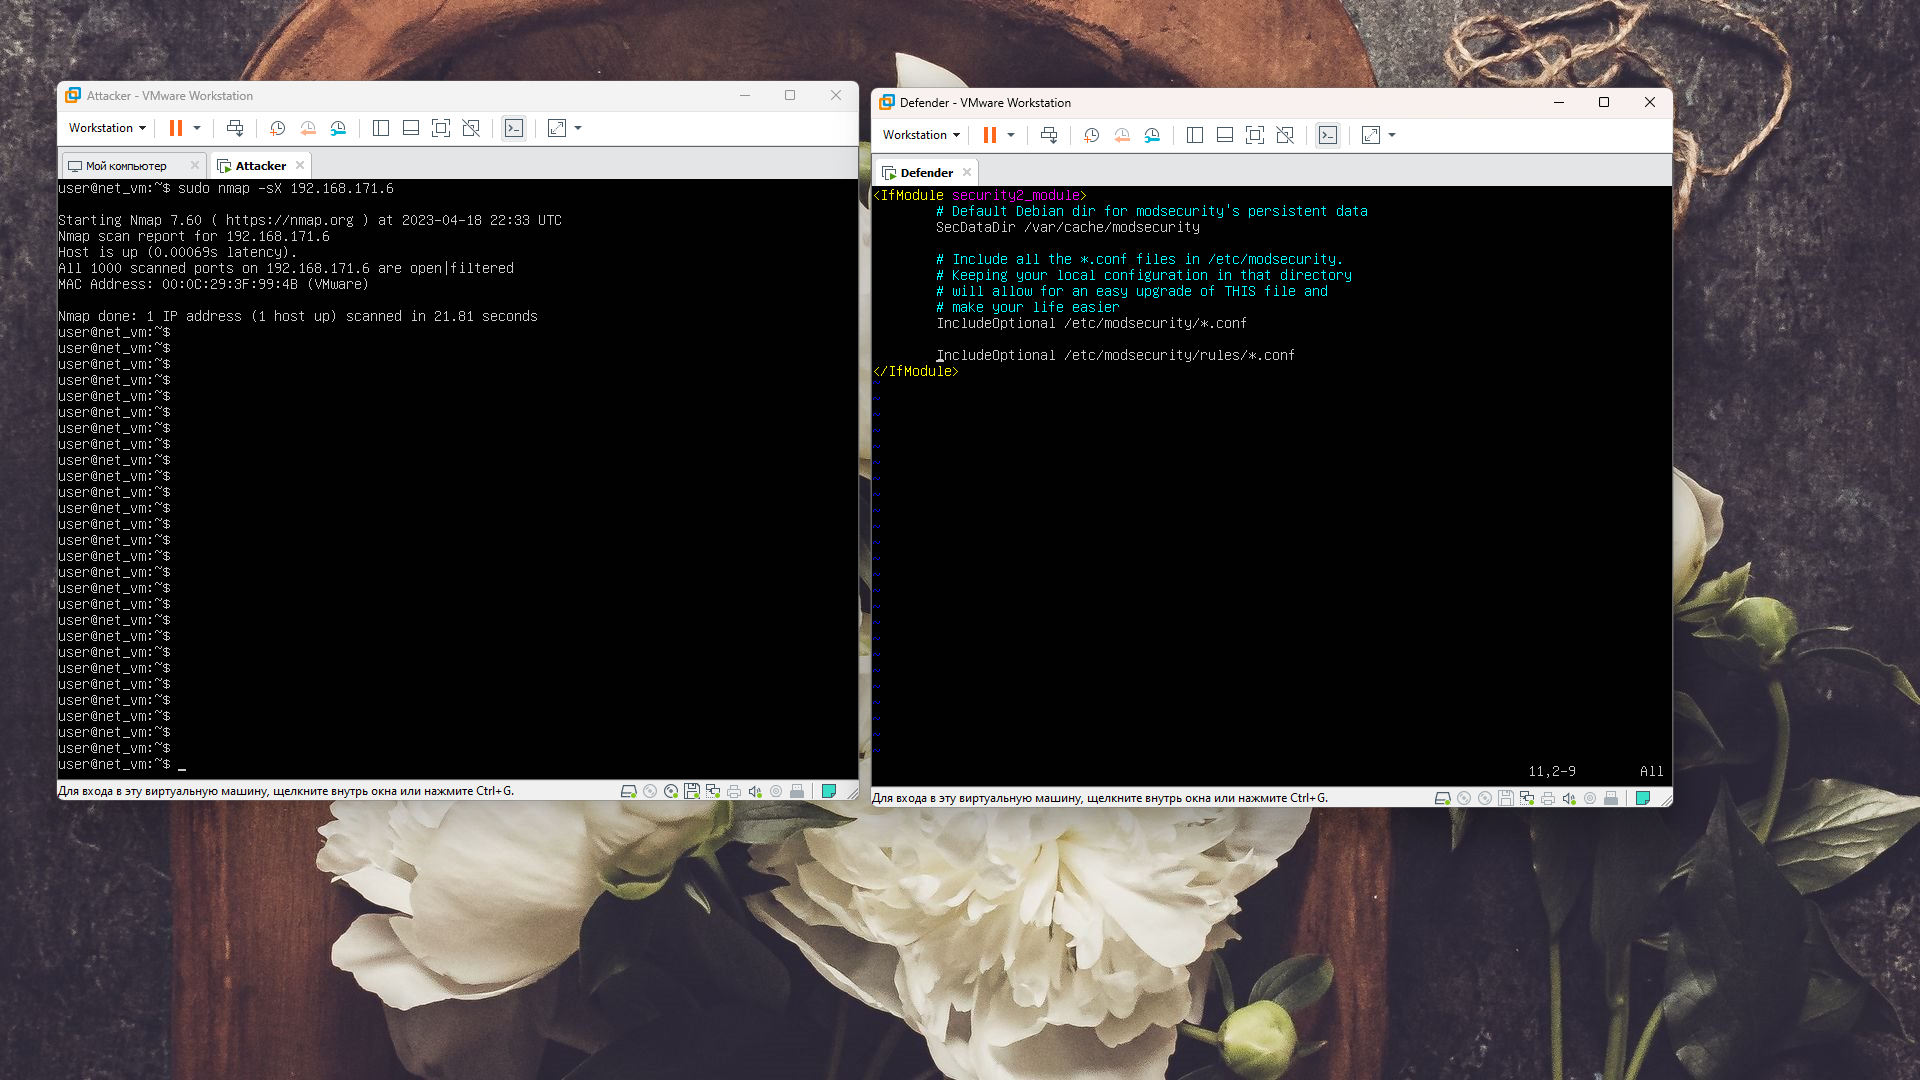
\includegraphics[width=0.85\textwidth]{03_00 (60)}
    \caption{Указываем путь до правил - \textit{/etc/modsecurity/rules}}
    \label{img:60}
  \end{figure}

  Теперь все настроено, осталось только перезапустить \textit{web}-сервер.
  Сделать это можно при помощи утилиты \textit{service}:
  \begin{minted}{bash}
    sudo service apache2 reload
    # А потом посмотреть состояние сервися
    sudo service apache2 status
  \end{minted}

  \begin{figure}[H]
    \centering
    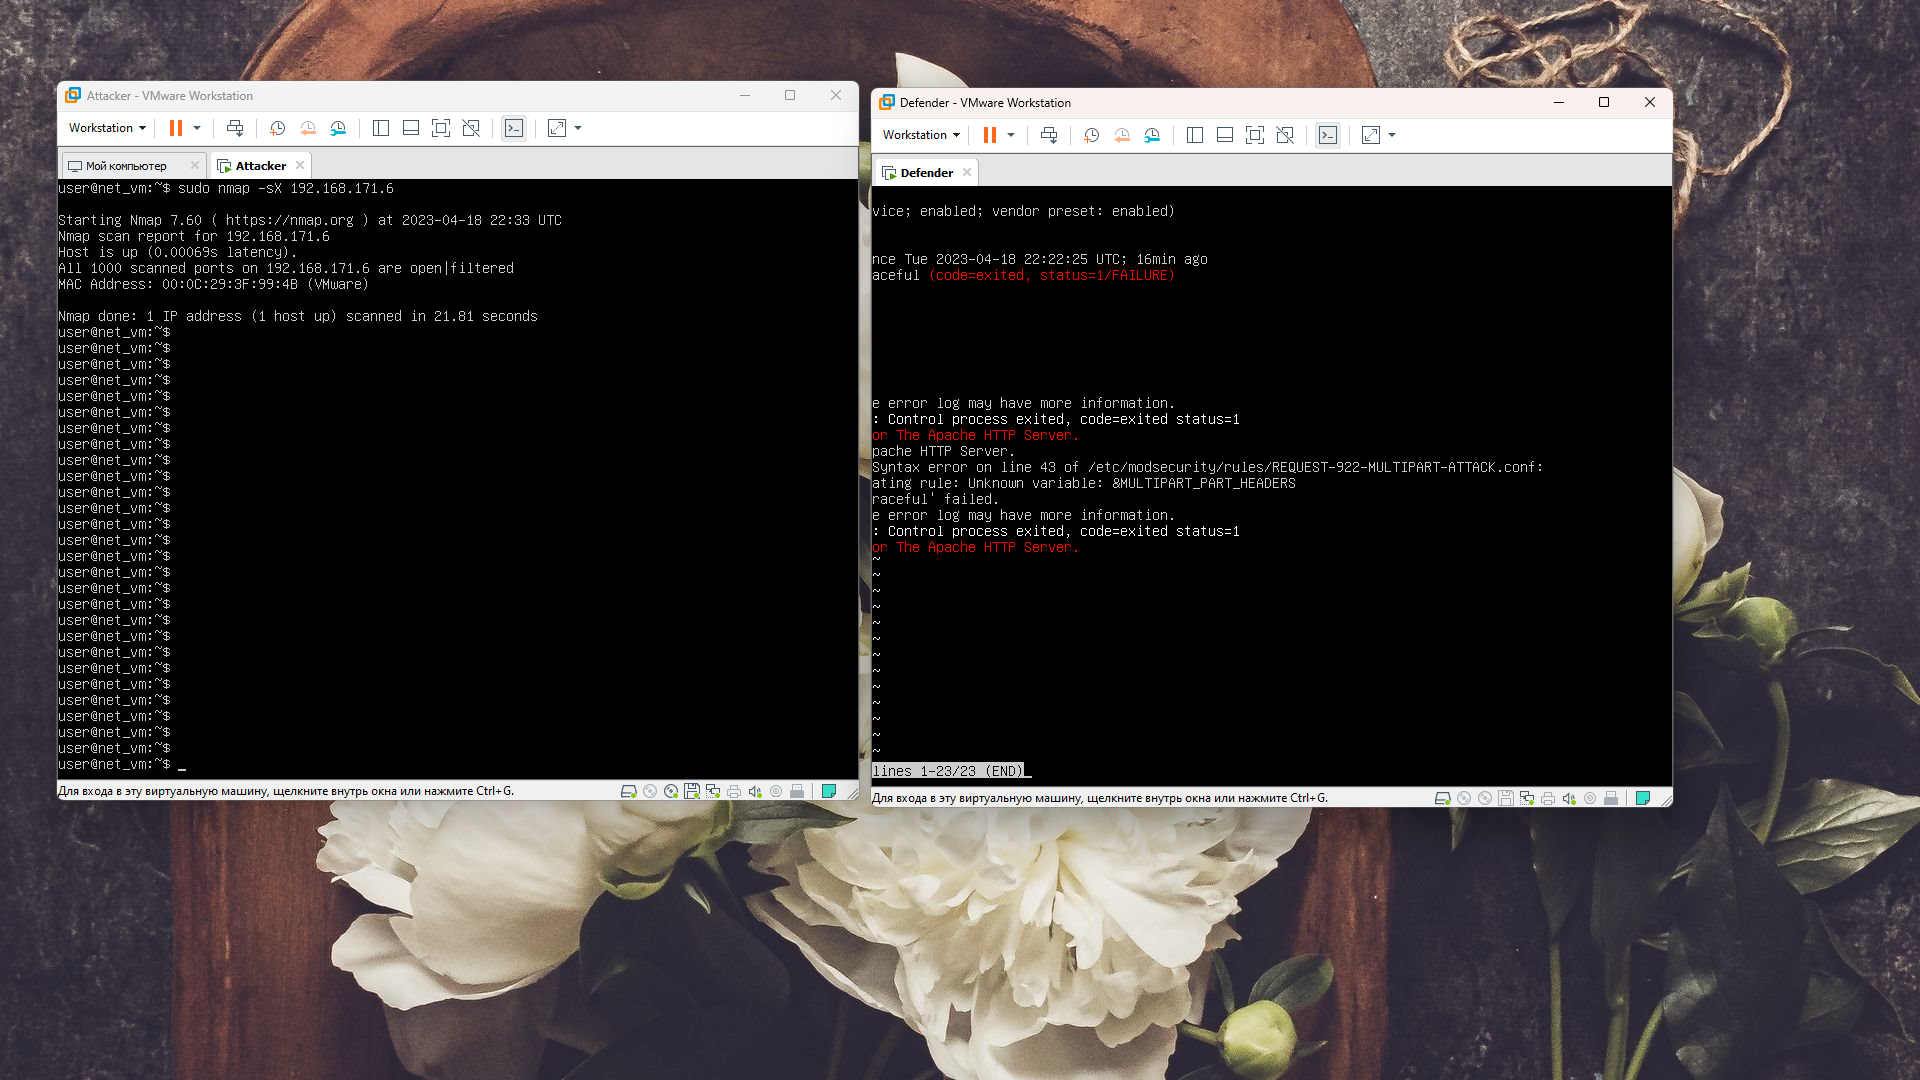
\includegraphics[width=0.85\textwidth]{03_00 (63)}
    \caption{Состояние сервиса после перезапуска}
    \label{img:63}
  \end{figure}

  Произошел конфликт версий - одно из установленных правил
  требует более новой версии \textit{web} сервера - удалим его (в логах указан путь до файла с ошибкой):

  \begin{figure}[H]
    \centering
    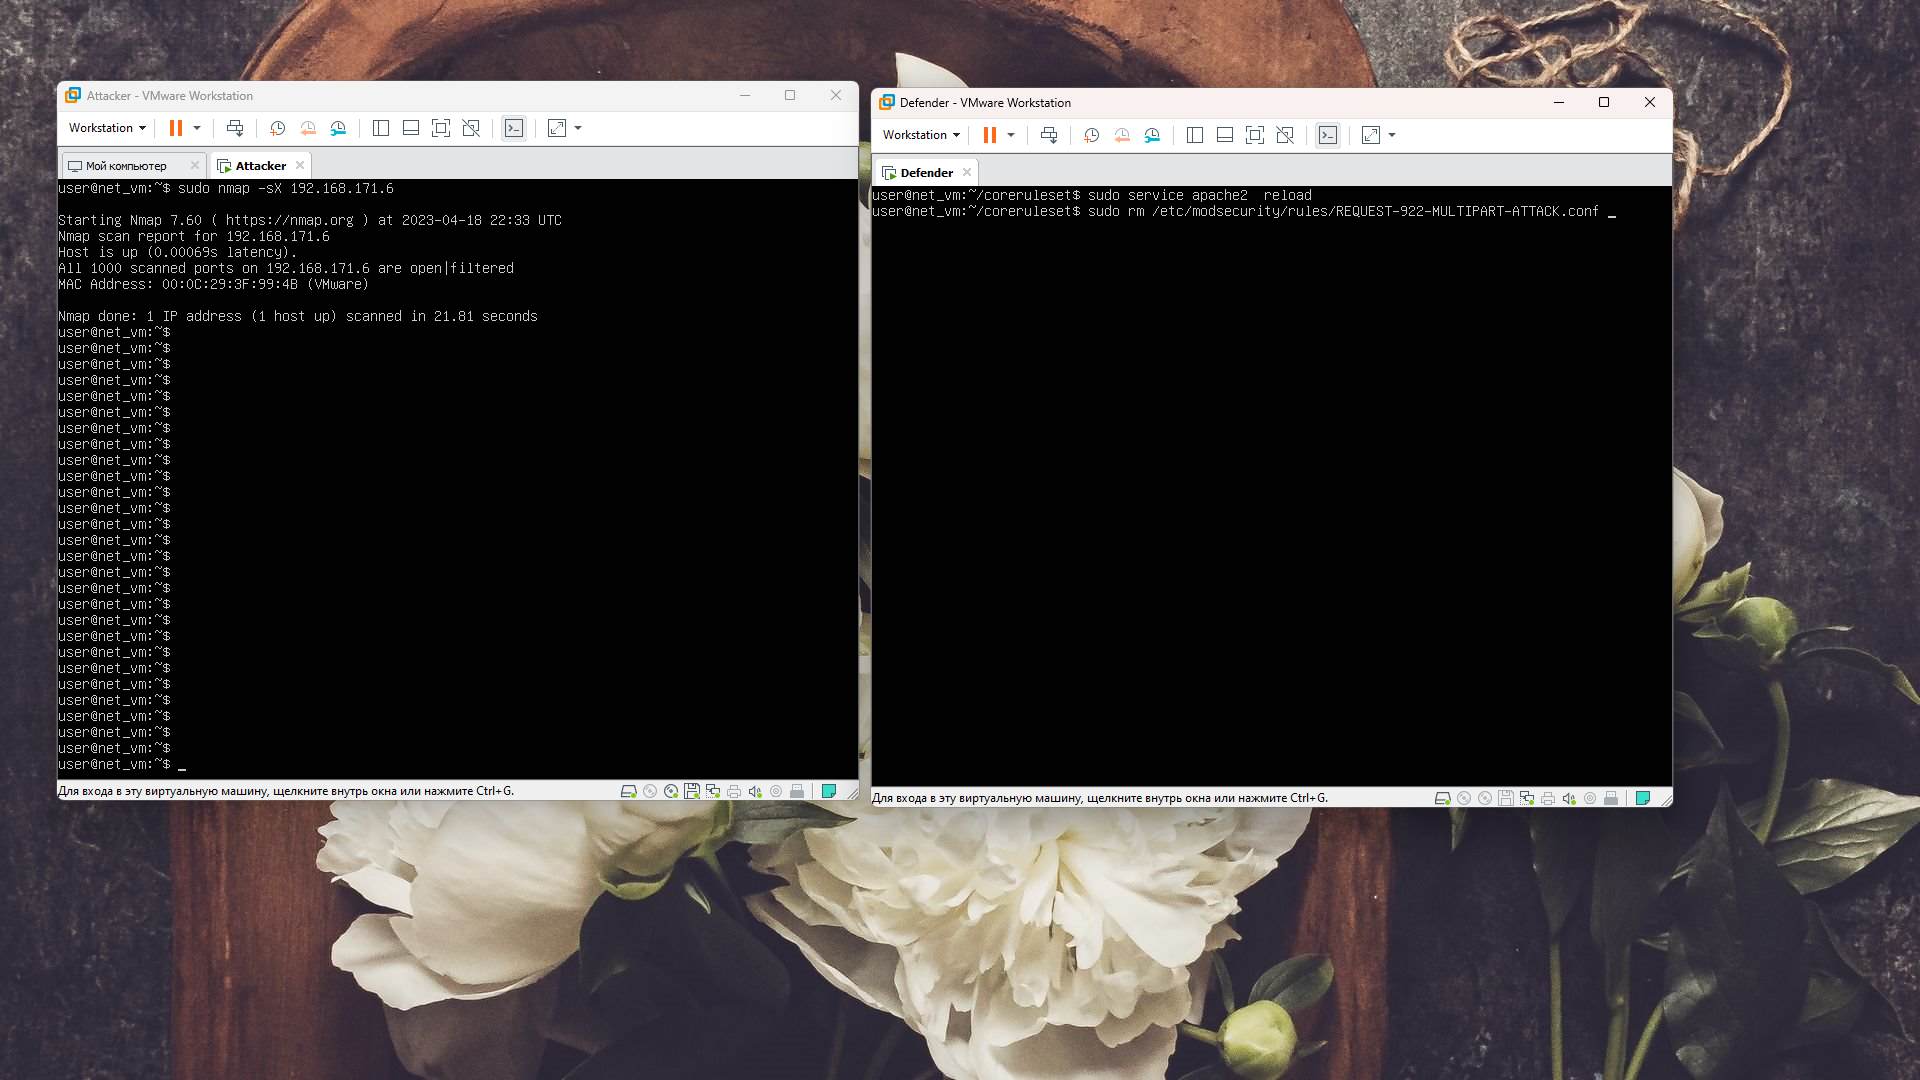
\includegraphics[width=0.85\textwidth]{03_00 (64)}
    \caption{Удаляем правило с ошибкой}
    \label{img:64}
  \end{figure}

  \begin{figure}[H]
    \centering
    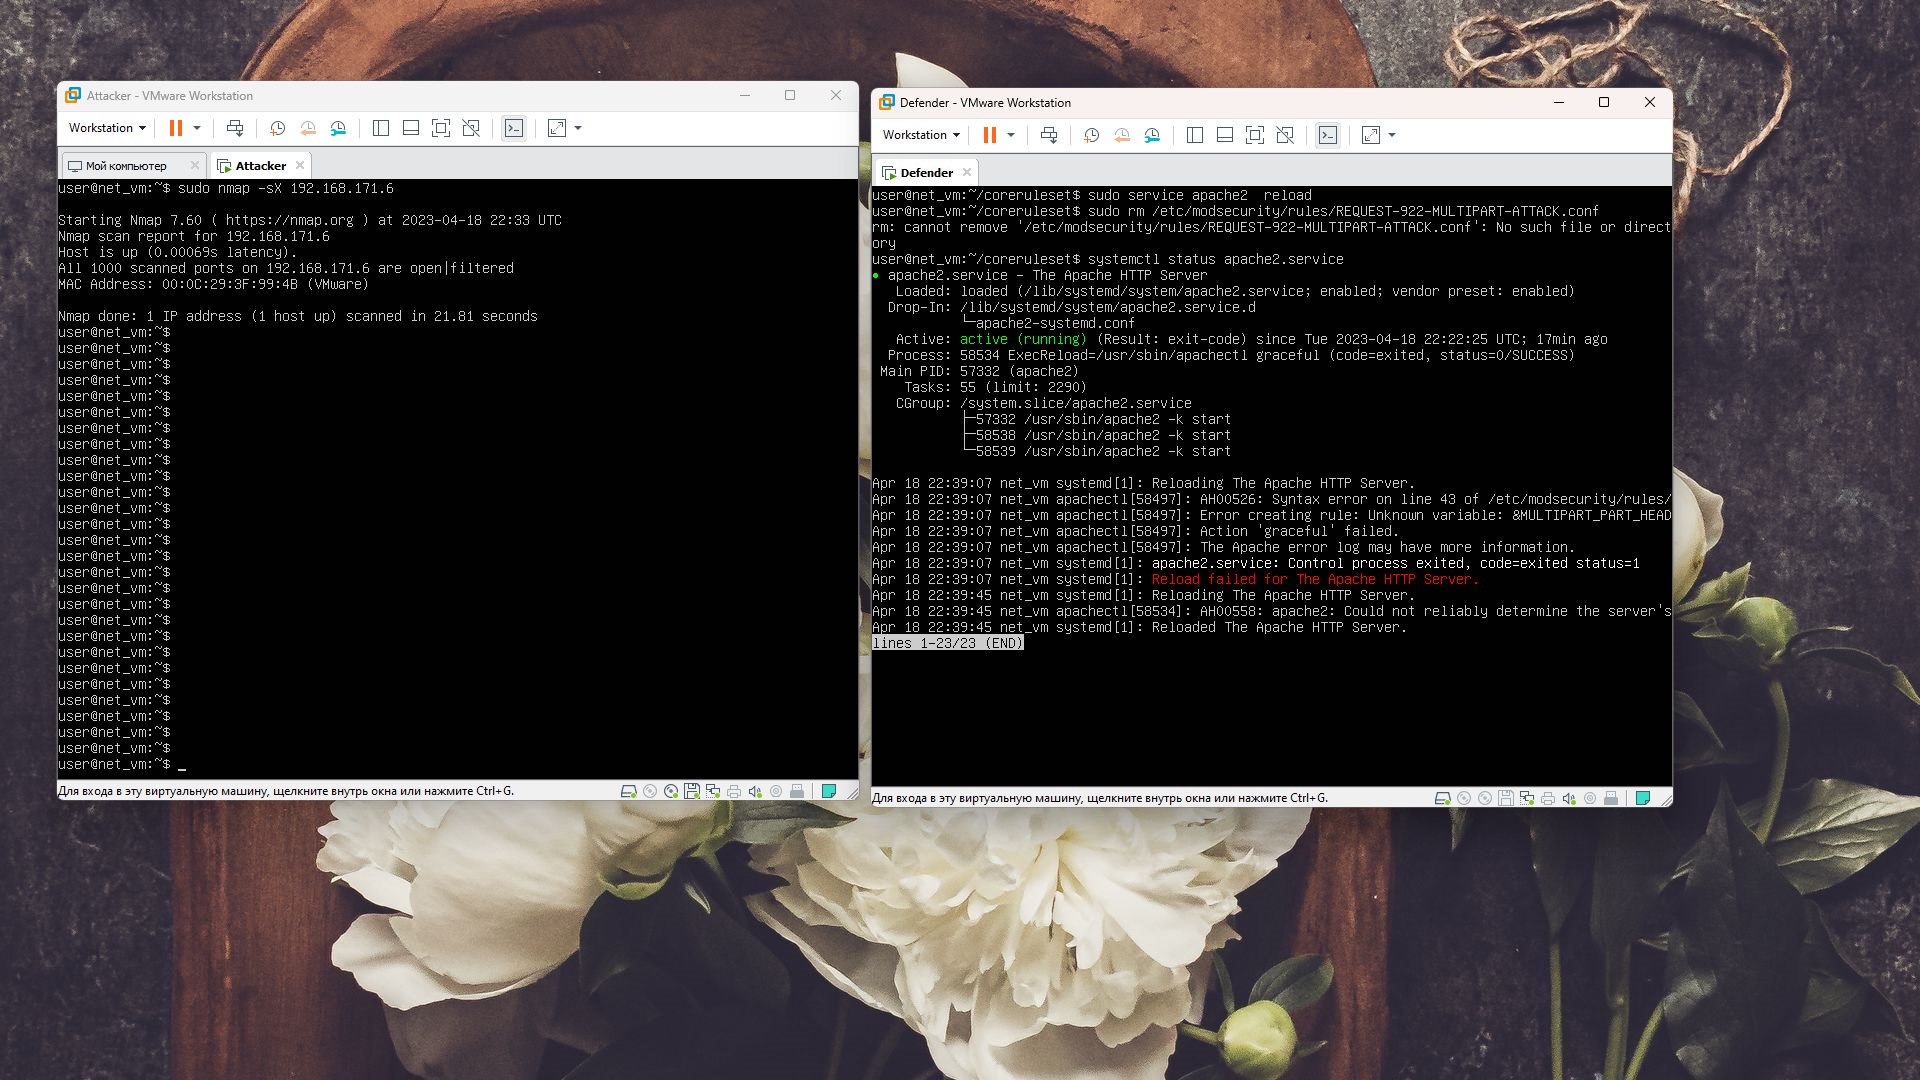
\includegraphics[width=0.85\textwidth]{03_00 (65)}
    \caption{Статус сервиса после перезапуска}
    \label{img:65}
  \end{figure}

  В логах все еще остались ошибки (от прошлого запуска), но статус сервиса \textit{running}, значит все работает.

  Все логи, касающие безопасности, будут записаны в специальный файл, посмотрим его содержимое:

  \begin{figure}[H]
    \centering
    \includegraphics[width=0.85\textwidth]{03_00 (66)}
    \caption{Пока запросов не было - тут пусто}
    \label{img:66}
  \end{figure}

  Теперь модуль безопасности не только установлен, но и настроен, запущен и работает,
  добавим новое правило - запретим все \textit{HTTP} запросы, в которых есть параметр \textit{testparam}
  с установленным в нем значением \textit{test}:

  \begin{figure}[H]
    \centering
    \includegraphics[width=0.85\textwidth]{03_00 (68)}
    \caption{Новое правило}
    \label{img:68}
  \end{figure}

  Если подобный запрос поступит, то сервер вернет ему ошибку с кодом 403.

  \begin{figure}[H]
    \centering
    \includegraphics[width=0.85\textwidth]{03_00 (69)}
    \caption{Снова перезагружаем сервис, чтобы все наверняка применилось}
    \label{img:69}
  \end{figure}

  А теперь попробуем выполнить запрос с таким параметром при помощи \textit{curl}:

  \begin{figure}[H]
    \centering
    \includegraphics[width=0.85\textwidth]{03_00 (71)}
    \caption{Запрос с параметром \textit{testparam=test}}
    \label{img:71}
  \end{figure}

  Как и ожидалось, сервер вернул ошибку с кодом 403, значит все настроено и работает верно.

  \section{Вывод}

  В ходе данной практической работы мною были получены навыки настройки фильтров
  для \textit{iptables} (сетевого экрана), а также правил для \textit{apache2 web}-сервера.

\end{document}

